%%%%%%%%%%%%%%%%%%%%%%%%%%%%%%%%%%%%%%%%%%%%%%%%%%%%%%%%%%%%%%%%%%%%
%% I, the copyright holder of this work, release this work into the
%% public domain. This applies worldwide. In some countries this may
%% not be legally possible; if so: I grant anyone the right to use
%% this work for any purpose, without any conditions, unless such
%% conditions are required by law.
%%%%%%%%%%%%%%%%%%%%%%%%%%%%%%%%%%%%%%%%%%%%%%%%%%%%%%%%%%%%%%%%%%%%

\documentclass[
  digital,     %% The `digital` option enables the default options for the
               %% digital version of a documeant. Replace with `printed`
               %% to enable the default options for the printed version
               %% of a document.
%%  color,       %% Uncomment these lines (by removing the %% at the
%%               %% beginning) to use color in the printed version of your
%%               %% document
  oneside,     %% The `oneside` option enables one-sided typesetting,
               %% which is preferred if you are only going to submit a
               %% digital version of your thesis. Replace with `twoside`
               %% for double-sided typesetting if you are planning to
               %% also print your thesis. For double-sided typesetting,
               %% use at least 120 g/m² paper to prevent show-through.
  nosansbold,  %% The `nosansbold` option prevents the use of the
               %% sans-serif type face for bold text. Replace with
               %% `sansbold` to use sans-serif type face for bold text.
  nocolorbold, %% The `nocolorbold` option disables the usage of the
               %% blue color for bold text, instead using black. Replace
               %% with `colorbold` to use blue for bold text.
  nolof,         %% The `lof` option prints the List of Figures. Replace
               %% with `nolof` to hide the List of Figures.
  nolot,         %% The `lot` option prints the List of Tables. Replace
               %% with `nolot` to hide the List of Tables.
]{fithesis4}
%% The following section sets up the locales used in the thesis.
\usepackage[resetfonts]{cmap} %% We need to load the T2A font encoding
\usepackage[T1,T2A]{fontenc}  %% to use the Cyrillic fonts with Russian texts.
\usepackage[
  main=english, %% By using `czech` or `slovak` as the main locale
                %% instead of `english`, you can typeset the thesis
                %% in either Czech or Slovak, respectively.
  english %% The additional keys allow
]{babel}        %% foreign texts to be typeset as follows:
%%
%%   \begin{otherlanguage}{german}  ... \end{otherlanguage}
%%   \begin{otherlanguage}{russian} ... \end{otherlanguage}
%%   \begin{otherlanguage}{czech}   ... \end{otherlanguage}
%%   \begin{otherlanguage}{slovak}  ... \end{otherlanguage}
%%
%% For non-Latin scripts, it may be necessary to load additional
%% fonts:
\usepackage{paratype}
\usepackage{todonotes}
\setuptodonotes{inline}
\usepackage{amssymb}
\usepackage{multirow}
\usepackage{array}
\usepackage{longtable}

%%
%% The following section sets up the metadata of the thesis.
\thesissetup{
    date        = \the\year/\the\month/\the\day,
    university  = mu,
    faculty     = fi,
    type        = bc,
    department  = Department of Computer Systems and Communications,
    author      = Tomáš Marek,
    gender      = m,
    advisor     = {Ing. Milan Brož, Ph.D.},
    title       = {Improvements to the Randomness Testing Toolkit},
    TeXtitle    = {Improvements to the Randomness Testing Toolkit},
    keywords    = {keyword1, keyword2, ...},
    TeXkeywords = {keyword1, keyword2, \ldots},
    abstract    = {%
      This is the abstract of my thesis, which can

      span multiple paragraphs.
    },
    thanks      = {%
      These are the acknowledgements for my thesis, which can

      span multiple paragraphs.
    },
    bib         = bibliography.bib,
    %% Remove the following line to use the JVS 2018 faculty logo.
    facultyLogo = fithesis-fi,
}
\usepackage{makeidx}      %% The `makeidx` package contains
\makeindex                %% helper commands for index typesetting.
%% These additional packages are used within the document:
\usepackage{paralist} %% Compact list environments
\usepackage{amsmath}  %% Mathematics
\usepackage{amsthm}
\usepackage{amsfonts}
\usepackage{url}      %% Hyperlinks
\usepackage{markdown} %% Lightweight markup
\usepackage{listings} %% Source code highlighting
\lstset{
  basicstyle      = \ttfamily,
  identifierstyle = \color{black},
  keywordstyle    = \color{blue},
  keywordstyle    = {[2]\color{cyan}},
  keywordstyle    = {[3]\color{olive}},
  stringstyle     = \color{teal},
  commentstyle    = \itshape\color{magenta},
  breaklines      = true,
}
\usepackage{floatrow} %% Putting captions above tables
\floatsetup[table]{capposition=top}
\usepackage[babel]{csquotes} %% Context-sensitive quotation marks
\begin{document}
%% The \chapter* command can be used to produce unnumbered chapters:
\chapter*{Introduction}
%% Unlike \chapter, \chapter* does not update the headings and does not
%% enter the chapter to the table of contents. I we want correct
%% headings and a table of contents entry, we must add them manually:
\markright{\textsc{Introduction}}
\addcontentsline{toc}{chapter}{Introduction}

Cryptography plays vital role in securing computer communication today. Many cryptographical primitives require to be set up using unique values (e.g. keys or nonces) to provide their functionality correctly. To acquire unique values, random number generators are used in practice.


% into - rng, random sequence 
Random number generators are tools for generating bit sequences with content that appears random. The desired properties \cite[p.~1-1]{nist_special} of such sequence are \emph{uniformity} (for each bit, the probability of both zero and one are exactly $1/2$), \emph{independence} (none of the bits is influenced by any other bit) and \emph{unpredictability} (it is impossible to predict next bit by obtaining any number of previous bits). 

% rng quality, tu01 guide - 2
The random number generators are of different quality in regard to fulfilling the desired properties of generated sequences. Each application of random number generators has different requirements for quality of the used generator. In cryptography, failure to fulfill the requirements may lead to compromising the security of the communication.

Therefore, there is need to assess the quality of the used random number generators. The assessment is done by mathematical analysis of the generator structure or by taking a sample output of the generator and applying a \emph{randomness test} \cite[p.~2]{tu01_guide}.

%Randomness testing is a form of statistical testing. It is used in cryptography to test the quality of the output of different cryptographic primitives such as (pseudo-)random number generators or ciphers, where the randomness of output is required. 

% intro to current state
Currently, there are several available programs for randomness testing. Most notable are the NIST STS\footnote{National Institute of Standards and Technology Statistical Test Suite} \cite{nist_site}, TestU01 \cite{tu01_site} and Dieharder \cite{dieharder_orig}. Providing a unified interface to the three are the Randomness Testing Toolkit (\emph{RTT}) \cite{rtt-site} and its evolution, the Randomness Testing Toolkit in Python (\emph{rtt-py})\cite{rtt-py-site}.

%The first goal of this thesis is to implement improvements into the \emph{rtt-py} so that it can fully replace the \emph{RTT}. These improvements include processing errors and warnings from the test batteries and extensions to the output format. The second goal is to make the randomness testing easier for new users with the explanation of randomness testing principles (Chapter \ref{theory}) and by creating the Configuration Calculator -- a tool that helps with the configurations of tests for both the \emph{RTT} and the \emph{rtt-py}.


% thesis goal - motivation of analysis

The \emph{RTT} contains flaws in regard to both usability and functionality. It might be replaced by the \emph{rtt-py} in the future, however, the two implementations are different. Therefore, the main goal of this thesis is to analyse the \emph{RTT} and the \emph{rtt-py} with focus on finding differences between the two implementations (particularly the features missing in \emph{rtt-py}) and on proposing improvements for both of the toolkits. 

% principles explanations
In Chapter \ref{chap:rand}, we explain the principles of randomness testing along with terms used in the following chapters. The aforementioned programs for randomness testing are presented in Chapter \ref{chap:sols}. In the first part of the analysis (described in Chapter \ref{chap: analysis}), we focus on improving the \emph{RTT} by analyzing the individual tests used by the \emph{RTT}. %This analysis resulted in creation of the Configuration Calculator -- tool for automated configuration of the \emph{RTT} based on the tested file.

%rtts analysis
The second part of the analysis (presented in Chapter \ref{chap:comparison}) is focused directly on \emph{RTT} and \emph{rtt-py}. In this part, we present and compare the output of \emph{RTT} and \emph{rtt-py}. Then, we analyse the features of both toolkits and list all differences found. Last, we propose several improvements that would extend the functionality of both \emph{RTT} and \emph{rtt-py}.

% RANDOMNESS TESTING - 'theoretical' chapter

\chapter{Randomness testing} \label{chap:rand}

The goal of this chapter is to provide an overview of the randomness testing process and to explain all used terms related to it. We present the two main approaches to the randomness testing -- the one-level and two-level tests. Both approaches are accompanied by application examples.

\section{Overview} \label{chap:rand-intro}

%Testing a sequence (define) (tu01guide - 1, tu01paper - 3, 17), required properties(nistspecial 1-1, 1-3 )

During a randomness test, a \emph{random sequence} is tested. In this document, we use the term random sequence to describe a finite sequence of zero and one bits, which was generated by a tested random number generator.  %\cite[p. 1-1]{nist_special} 

%Null/alternative hypothesis (tu01paper - 3, možná učebnice)
%Randomness testing as statistical testing (tu01guide - 2)

Randomness test is a form of \emph{empirical statistical test} \cite[p. 2]{tu01_guide}, where we test our assumption about the tested data - the \emph{null hypothesis} ($H_0$). The \emph{null hypothesis} states that the sequence is \emph{random} (i.e. was generated by a perfect random number generator). Associated with the null hypothesis is the \emph{alternative hypothesis} ($H_1$), which states that the sequence is \emph{non-random} (i.e. was generated by a biased random number generator). The goal of the test is to search for evidence against the null hypothesis. 

%Idea of testing – extremeness of a sample ? (nistspecial - 1-3+)

%result (accept, reject, Type I/II error) (nistspecial - 1-3+, učebnice 416)

The result of the test is either that we \emph{accept} the null hypothesis (the sequence is considered random), or that we \emph{reject} the null hypothesis (and accept the alternative hypothesis - the sequence is considered non-random) \cite[p. 417]{basic_practice}. We reject the null hypothesis when the evidence found against the null hypothesis is strong enough, otherwise we accept it. Note, that two different tests may produce different results while testing the same sequence because each test examines the randomness using different aspects. Based on the true situation of the null hypothesis, four situations depicted in Table \ref{tab:type_errors} may occur.

\begin{table}
  \begin{tabularx}{0.7\textwidth}{l|c|c}
    %\toprule
    TRUE  & \multicolumn{2}{c}{TEST CONCLUSION}\\
    SITUATION &Accept $H_0$ & Reject $H_0$\\
    \midrule
    $H_0$ is True &  No error & Type I error  \\
    $H_0$ is False & Type II error & No error \\
    %\bottomrule
  \end{tabularx}
  \caption{Possible situations when assessing the result of a statistical test regarding the test result and the true situation.}
  \label{tab:type_errors}
\end{table}

\section{Single-level testing} \label{chap:rand-single}
%significance level (tu01 paper 5-8, nistspecial 1-3+, rec for stat testing 5, učebnice)

A single-level test examines the random sequence directly (compare with the two-level test in Section \ref{chap:rand-two_level}). Before the test user must choose a \emph{significance level}, which determines how strong the found evidence has to be to reject the null hypothesis. The test yields a \emph{p-value}, which is used to accept or reject the null hypothesis.

The \emph{significance level} ($\alpha$) is crucial to assessing the test result and must be set before the test. The $\alpha$ is equal to the probability of Type I Error. Usual values are $\alpha = 0.05$ or $\alpha = 0.01$ \cite[p. 390]{basic_practice}, for use in testing of cryptographic random number generators lower values may be chosen \cite[p. 1-4]{nist_special}. The lower $\alpha$ is set, the stronger the found evidence has to be to reject the null hypothesis. %(cite? derived from nistspecial 1-4)

%Test statistic (= function, known distribution), sample (tu01 paper 4+)

The randomness test is defined by a \emph{test statistic} $Y$ \cite[p.~4]{tu01_paper}, which is a function of a finite bit sequence. The distribution of its values under the null hypothesis must be known (or at least approximated). The value of the test statistic ($y$) is computed for the tested random sequence. Each test statistic searches for the presence or absence of some ``pattern'' in the sequence, which would show the non-randomness of the sequence. There is an infinite number of possible test statistics, therefore no group of tests can guarantee that the sequence is truly random.

%p-value (one, two tailed, how extremeness is set) (nist-opt 5, nist-special 1-4,rec for stat testing 5)

The \emph{p-value} denotes the probability of the test statistic $Y$ taking value at least as extreme as the observed $y$, assuming that the null hypothesis is true. In randomness testing, it is equal to the probability that a \emph{perfect random number generator} would generate ``less'' random sequence. The smaller is the p-value, the stronger is the found evidence against the null hypothesis \cite[p. 386]{basic_practice}. The p-value is calculated based on the observed $y$.



\subsection{Result interpretation} \label{chap:rand-interpretation}
%interpratation (učebnice 380-400)

The decision about the test result is based on the computed \emph{p-value} \cite[p. 390]{basic_practice}. If the p-value is lower than the $\alpha$, we \emph{reject the null hypothesis} (and accept the alternative hypothesis), because strong enough evidence against the null hypothesis was found. If the p-value is greater than or equal to the $\alpha$, we \emph{accept the null hypothesis}, because the evidence against the randomness was too weak. It is sometimes recommended to report the \emph{p-value} as well instead of accept/reject only, as it yields more information \cite[p. 90]{tu01_guide}.

The p-values close to $\alpha$ can be considered \emph{suspicious} because they do not clearly indicate rejection. Further testing of the random number generator on \emph{other} random sequences is then in place to search for further evidence \cite[p.~5]{tu01_paper}. The reason is that \emph{randomness} is a probabilistic property, therefore even the perfect random number generator may generate a non-random sequence with a low p-value (although it is very unlikely). The further evidence is used to differentiate between the bad generator generating a non-random sequence systematically and the good generator generating a non-random sequence by ``chance'' \cite[p. 90]{tu01_guide}.

%example
\subsection{Example} \label{chap:rand-example}

To demonstrate how a single one-level randomness test is made, the Frequency (Monobit) Test \cite[p. 2-2]{nist_special} from the NIST STS battery was chosen.  This test is based on testing the fraction of zeroes and ones within the sequence. For a random sequence with length $n$, the count of ones (and zeroes) is expected to be around $n/2$ (the most probable values are close to $n/2$). 

For the Monobit Test NIST recommends that the tested sequence has at least 100 bits. The test statistic $Y=S_{obs}$ of the Monobit test is defined as:
\[S_{obs} = \dfrac{|\#_1 - \#_0|}{\sqrt{n}},\]
where $\#_1$ represents the count of ones in the tested sequence (similarly for zeroes) and $n$ is the length of the tested sequence. Under the null hypothesis, the reference distribution of $S_{obs}$ is half normal (for large $n$). The p-value is computed as:
\[ p = erfc\biggl(\dfrac{S_{obs}}{\sqrt{2}}\biggr),\]
where $erfc$ denotes the \emph{complementary error function} used to calculate probabilities for the normal distribution.

 Let
\[\begin{split}
    \epsilon = 10011001010010000010001001011001101100001101000111\\10101001010010010011100111001100110010010100111011
\end{split}\]
 be the tested sequence. Then the test statistic for this sequence equals to:
 \[y = \dfrac{|46 - 54|}{\sqrt{100}}\ = \dfrac{|-8|}{10} = 0.8,\]
 and the p-value (visualised at Figure \ref{fig:example}) is: 
 \[p = erfc\biggl(\dfrac{0.8}{\sqrt{2}}\biggr) \approx 0.423.\]

% TODO dedice only one alpha?
To interpret the test, we compare the computed \emph{p-value} to the chosen $\alpha$. The $\emph{p-value} \approx 0.423$ is greater than both usual $\alpha = 0.05$ and $\alpha = 0.01$, therefore we accept the null hypothesis for both \emph{significance levels} and the sequence $\epsilon$ is considered random.

\begin{figure}[H]
  \begin{center}
    %% minimus is about 100 pixels per 1 centimeter or 300 pixels per 1 inch.
    %% The optimum is about 250 pixels per 1 centimeter 
    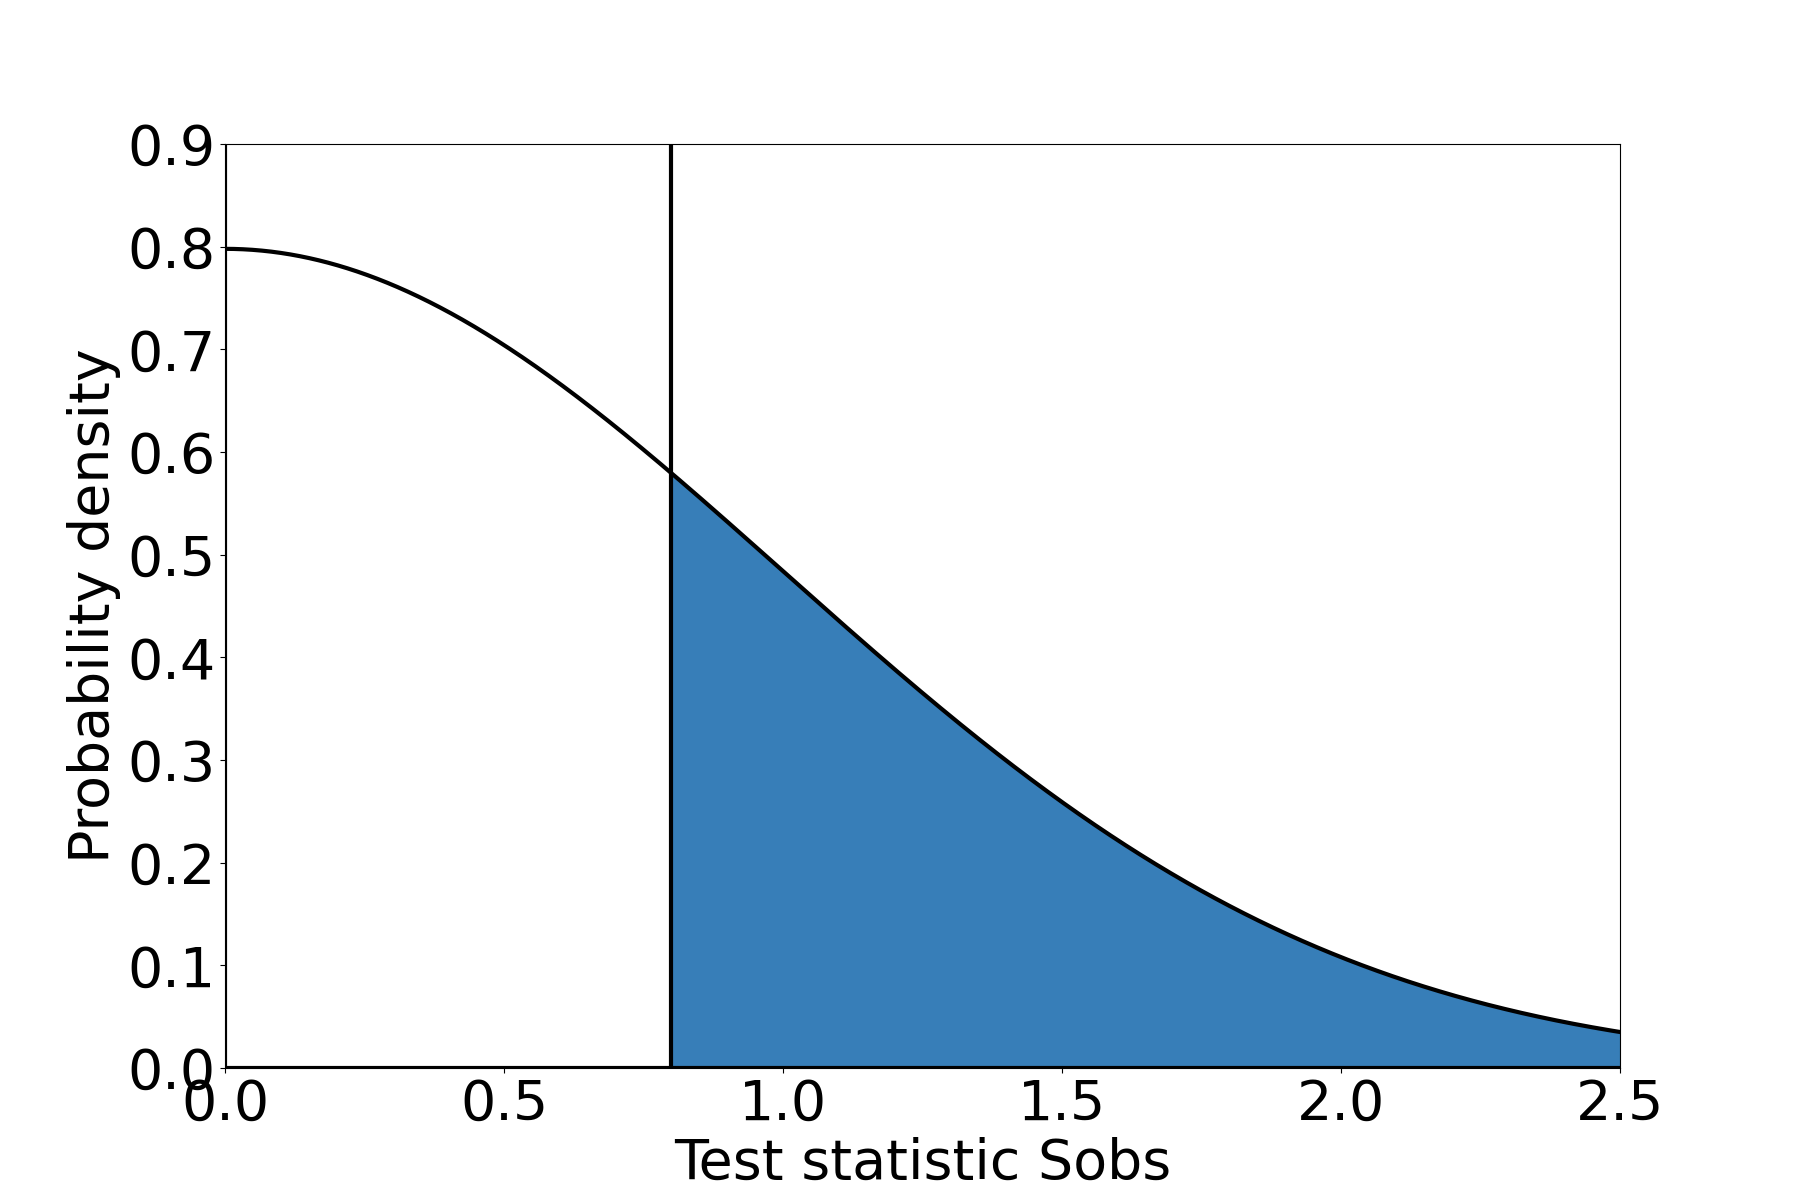
\includegraphics[width=8cm]{figures/test_example.png}
  \end{center}
  \caption{Visualization of the Monobit Test example p-value for test statistic value $y = 0.8$}
  \label{fig:example}
\end{figure}

\pagebreak
% two-level (tu01guide 88, tu01paper 5-8, correcting_dieharder 14)
%%%%%%%%%%%%%
% two-level
%%%%%%%%%%%%
\section{Two-level testing} \label{chap:rand-two_level}

% two-level motivation (tu01_paper 5-8)
The \emph{two-level test} is done by repeating the single-level test $n$ times. The important part is comparing the distribution of produced p-values to the expected distribution \cite[p.~7]{tu01_paper}. The two-level test allows the random sequence to be examined both locally and globally, while (in general) the single-level test examines the sequence only on the global level. This may lead to discovering local patterns, which cancel out on the global level. 

To apply the two-level test the tested sequence is split into $n$ equal-length disjoint subsequences. The same single-level test is applied to each of the subsequences (as described in Section \ref{chap:rand-single}) and its p-values are collected, resulting in a set of $n$ p-values. The tests are called \emph{first-level tests} and the p-values are called \emph{first-level p-values}.\footnote{Note that the first-level p-values are not subject to accept/reject decision.} Under the null hypothesis, the first-level p-values of a given test statistic are uniformly distributed over the interval $(0,1]$ \cite[p. 14]{bad_day}.

% GOF  - 1
The crucial part of the two-level test is examining the distribution of \emph{observed first-level p-values}. Usually, the \emph{goodness-of-fit} (GOF) test is applied as the \emph{second-level test} \cite[p. 6]{tu01_paper}. GOF tests are a family of methods used for examining how well a data sample fits a given distribution \cite[p. 1]{GOF-techniques}. The most used GOF tests in randomness testing are the $\chi^2$ (chi-squared) and Kolmogorov-Smirnov test. Other notable tests are the Anderson-Darling and Cramér-von-Mises tests. %\cite[p. 14]{bad_day}

The second-level test is defined by a test statistic $Y$, which is a function of the first-level p-values. Test statistic value ($y$) is calculated from the observed \emph{first-level p-values} and then the \emph{second-level p-value} is calculated from $y$. At last, the second-level p-value is interpreted as in the one-level test (as described in Section \ref{chap:rand-interpretation}). 

% ratio of passed sequences
Alternatively, a \emph{proportion of subsequences passing the first-level test} is used by NIST STS to examine the fist-level p-values uniformity. Under the null hypothesis, it is expected for $n\cdot\alpha$ subsequences to \emph{be rejected} (i.e. to have p-value $< \alpha$) by the first-level test (be subject to a Type I Error). The ratio of sequences passing the first-level test is expected to be around $1-\alpha$, any different ratio indicates non-uniformity of observed first-level p-values \cite[p. 4-2]{nist_special}. No p-value is reported in this case, only the ratio.

% GOF comparison?: (rec_for_stat 6)

% KS - description - (para and nonpara - 171)
\subsection{Kolmogorov-Smirnov test}
The (one-sample) Kolmogorov-Smirnov (KS) test is used in randomness testing to compare the observed first-level p-values to the uniform distribution. The Kolmogorov-Smirnov test is built on comparing the cumulative distribution function (CDF)\footnote{For a given distribution and value $x$, the CDF returns the probability of drawing a value less than or equal to $x$.} of the expected distribution and the empirical cumulative distribution function (eCDF)\footnote{For a set of observed data and value $x$, the eCDF returns the probability of drawing a value less than or equal to $x$.} of the observed samples \cite[p. 100]{GOF-techniques}. %cdf - nist_special 1-5 

%TODO test statistics
In the first variant, two test statistics are calculated. The test statistic $D^+$ ($D^-$) is the maximal vertical distance between CDF and eCDF above (under) the CDF. In the second variant, only the test statistic $D$ (maximal vertical distance between CDF and eCDF) is measured. Formally, the test statistics are defined as
\[\begin{split}
    &D^+ = sup_x\{F_n(x) - F(x)\}\\
    &D^- = sup_x\{F(x) - F_n(x)\}\\
    &D \:\:\:= sup_x\{|F_n(x) - F(x)|\} = max(D^+, D^-)
\end{split}
\] where $F(x)$ is the CDF and $F_n(x)$ is the  eCDF.


\begin{figure}
  \begin{center}
    %% minimus is about 100 pixels per 1 centimeter or 300 pixels per 1 inch.
    %% The optimum is about 250 pixels per 1 centimeter 
    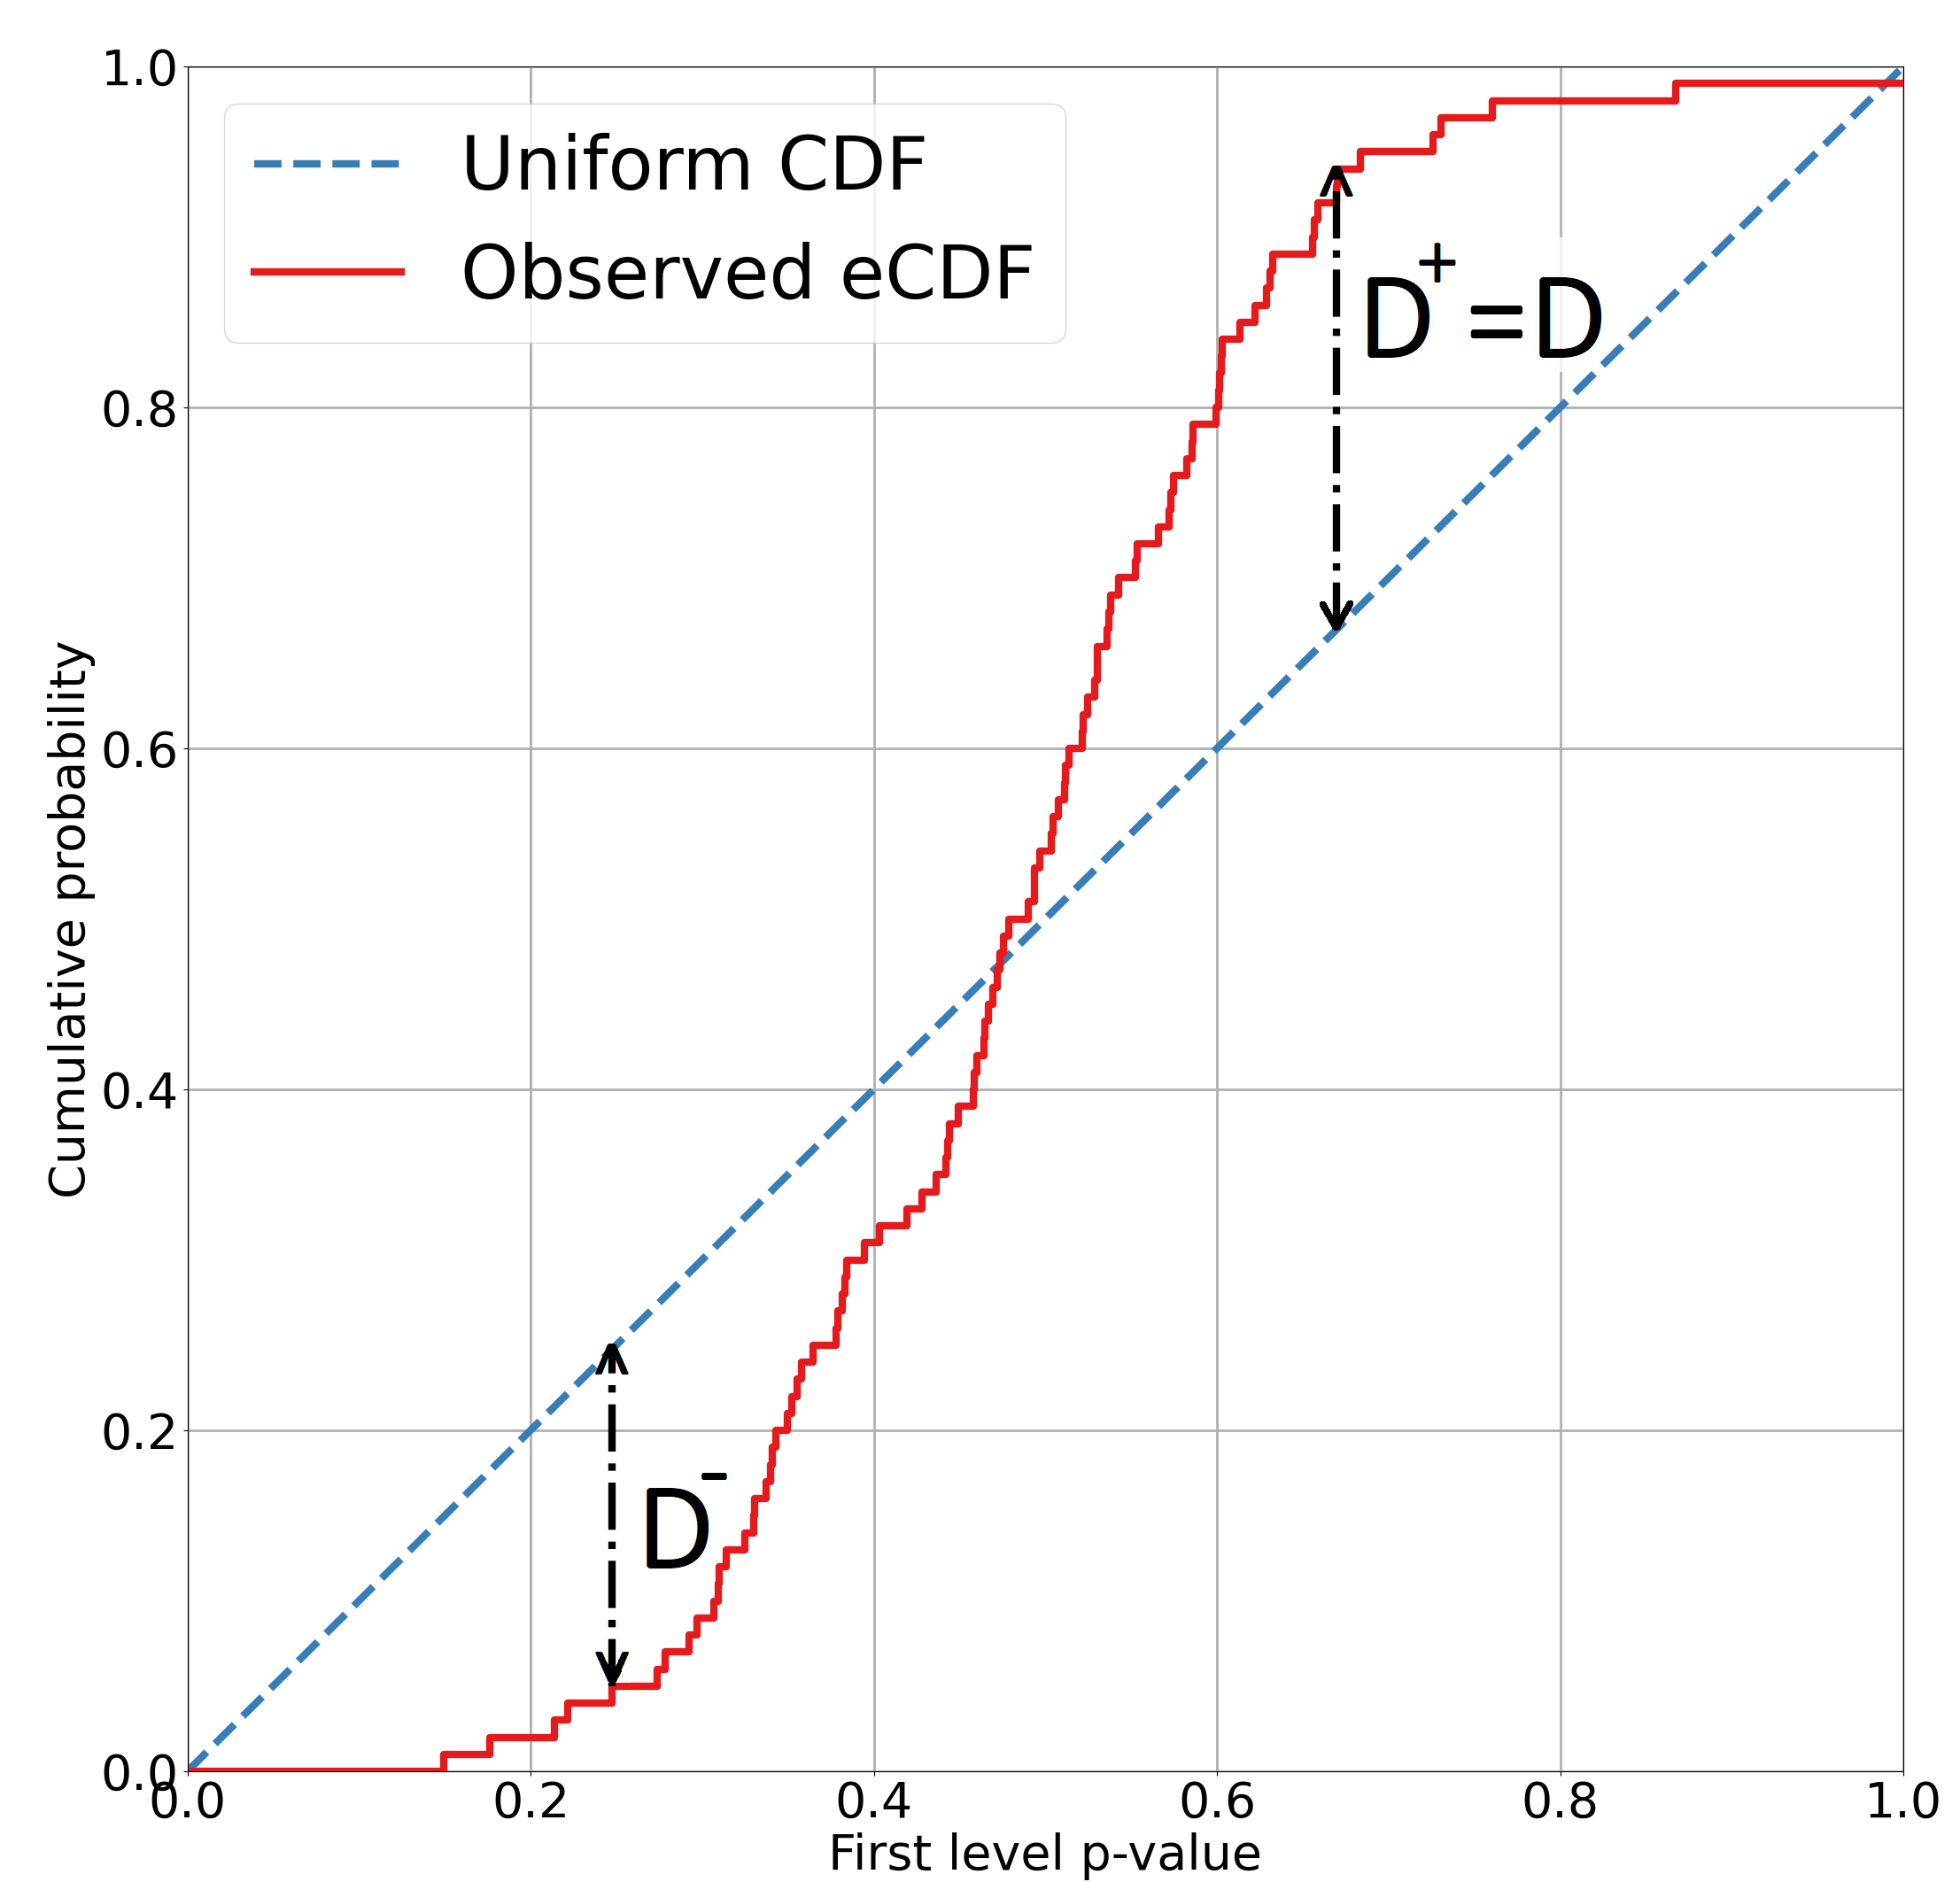
\includegraphics[width=9cm]{figures/ks_d.png}
  \end{center}
  \caption{Visualization of Kolmogorov-Smirnov test statistics for expected uniform distribution and observed data sample.}
  \label{fig:ks_d}
\end{figure}

% $\chi^2$ description (GOF - 100)
\subsection{Chi-squared test}

The (Pearson's) $\chi^2$ test is used to find a statistically significant difference between frequencies of categories in two sets of categorical data \cite[p. 171]{stat-procedures}. The first-level p-values are split into $k$ bins (categories) and their respective frequencies are counted. The counted frequencies are compared to the expected frequencies.

For data with $k$ categories the test statistic $\chi^2$ is defined as:
\[\chi^2 = \sum_{i=1}^{k} \dfrac{(x_i - m_i)^2}{m_i}, \]
where $x_i$ is the observed frequency in $i$-th category and $m_i$ is the expected frequency in $i$-th category. %For first-level p-values, the expected frequency is equal in each interval.
For a correct test, the expected frequency in each category must be at least five.

% Two-level example
\subsection{Example}

In the two-level test example, we will test one sequence using both one and two-level tests to demonstrate the difference between them. First, the sequence is tested using the one-level Frequency (Monobit) test from the NIST STS battery.\cite[p. 2-2]{nist_special} Then the same sequence is assessed by the two-level test using the Frequency test as the first-level test and KS and $\chi^2$ tests as the second-level test. Let
\[\begin{split}
    \epsilon =\:15\: &* (100\:consecutitive\:zeroes) + \\
    15\:&*\:(100\:alternating\:ones\:and\:zeroes) + \\
    5\:&*\:(55\:zeroes\:and\:45\:ones)\:+\:\\
    15\:&*\:(100\:consecutive\:ones)
\end{split}\]
be the tested sequence. 

The result of the one-level Frequency test for the sequence $\epsilon$ is p-value $\approx 0.479$. The null hypothesis is accepted for both usual $\alpha = 0.01$ and $\alpha = 0.05$ and the sequence $\epsilon$ is considered random. The sequence $\epsilon$ however clearly contains a pattern, therefore the probability of it being generated by a perfect random number generator is very low.

For the two-level test, the sequence $\epsilon$ is split into $n=50$ disjoint 100-bit long subsequences. The Monobit test is applied on each subsequence resulting in a set of first-level p-values shown in Table \ref{tab:first_pvalues}.

\begin{table}[h]
  \begin{tabularx}{0.4\textwidth}{ll}
    \toprule
    p-value & occurrences  \\
    \midrule
    $1.52 \cdot 10^{-23}$ & $30$\\
    $0.31$ & $5$\\
    $1.0$ & $15$\\
    \bottomrule
  \end{tabularx}
  \caption{First-level p-values produced by the Monobit Test over the 50 100-bit long subsequences of the sequence $\epsilon$.}
  \label{tab:first_pvalues}
\end{table}

The last step is to apply the GOF tests. The first applied test is the $\chi^2$ test with $k=10$ equal-width categories, the expected frequency of p-values in each category is five. The test statistic:
\[\chi^2 = \sum_{i=1}^{10} \dfrac{(x_i - 5)^2}{5} = 180,\]
corresponds to p-value $p\approx5.06\cdot10^{-34}$. The null hypothesis is rejected for both $\alpha = 0.01$ and $\alpha = 0.05$. 

Next, the Kolmogorov-Smirnov test is applied. The eCDF is calculated and then the D statistic is computed. The test statistic $D = 0.6$ correspond to p-value $\approx 9.63\cdot10^{-18}$. Again, the null hypothesis is rejected for both $\alpha = 0.01$ and $\alpha = 0.05$, and the sequence is considered non-random.

\begin{figure}[h]
  \begin{center}
    %% minimus is about 100 pixels per 1 centimeter or 300 pixels per 1 inch.
    %% The optimum is about 250 pixels per 1 centimeter 
    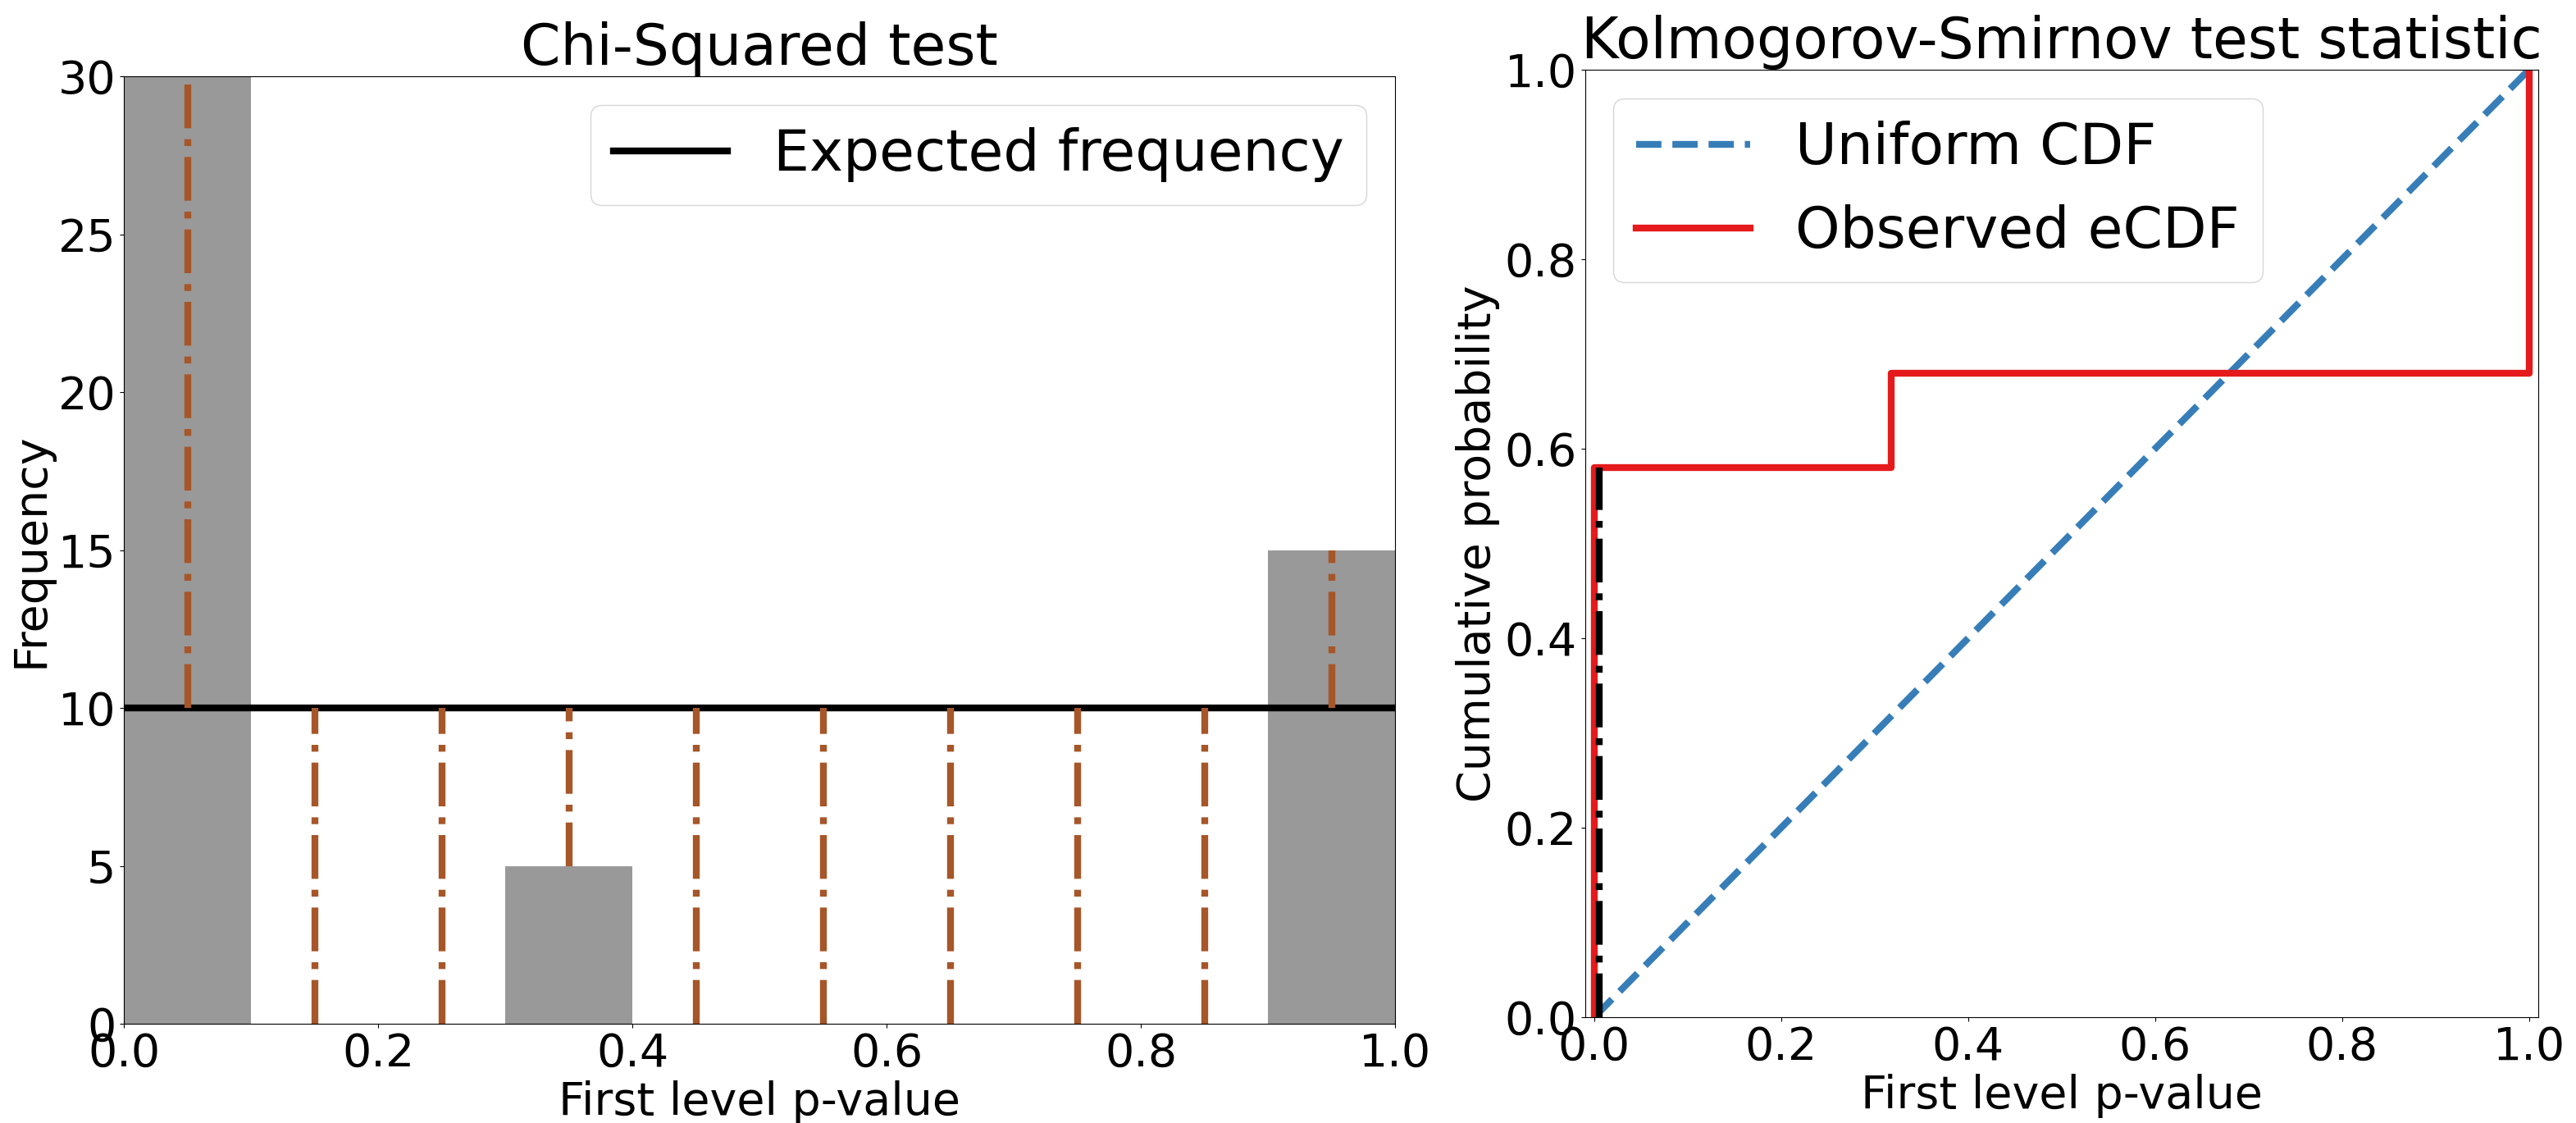
\includegraphics[width=12.5cm]{figures/two_example.png}
  \end{center}
  \caption{Visualisations for $\chi^2$ and KS tests for two-level test example.}
  \label{fig:two_example}
\end{figure}

%%%%%%%%%%%%%%%%%%%%%
%AVAILABLE SOLUTIONS
%%%%%%%%%%%%%%%%%%%%%

\chapter{Programs for randomness testing} \label{chap:sols}
In this chapter, available programs for randomness testing are presented. First section describes \emph{statistical testing suites} (often referred to as batteries). The second section shows \emph{randomness testing toolkits}, which encompass several batteries together. Overview of setup and output is given in both sections.

\section{Statistical testing batteries} \label{chap:sols-batteries}
%battery, individual test - mapping to test statistic
%Mention overflow detection
%If there are any problems with the battery (e.g. tests which read different amount of data from DieHarder). -
%how batteries interpret results (first/second level, more statistics)
%strong and weak things 
%describe output / image
%General description of battery - set of tests, choose test by ID, set tested file \\
%individual test - smallest executable part, possibly more test statistics, setting of the test(ntup, bitw...), data consumption (fixed vs set by user), number of first levels, return-first level pvalues, second-level p-value,


% (Obratil 2, tu01 guide 5)

\emph{Statistical testing battery (suite)} is a set of randomness tests with predefined parameters that allows the user to conveniently apply randomness tests \cite[p. 5]{tu01_guide}. Because all of the batteries share significant similarities, an \emph{abstract battery} is presented to demonstrate the principles. Then, each battery is presented in more detail, mapping its features to the \emph{abstract battery}. The described batteries are Dieharder, NIST STS, FIPS, BSI, and several batteries from TestU01.


An \emph{abstract battery} consists of $n$ individual tests, which are distinguished by \emph{test IDs}. Usually, one individual test maps to one two-level test. Some individual tests consist of more \emph{subtests}, which are all executed at once when the individual test is executed.

\todo{rewrite better the example}
Each \emph{subtest} maps to one \emph{two-level test}. The first-level test statistics of subtests are usually related to each other by using the same operation on the tested sequence. For example, the Diehard Craps Test \cite{dieharder_orig} plays 200~000 games of craps. The two calculated first-level test statistics are based on a count of wins and GOF test of distribution of throws needed to end the game. 

\emph{Variant of the test} is an individual test that is parametrized to search for modified patterns in the data. Only some individual tests allow such parametrization. Usually, all possible \emph{variants} of a given individual test are executed.  \cite[p. 2]{vavercak}

The following settings are available in \emph{abstract battery}. They can be set either \emph{globally} with same values for all \emph{individual tests}, or \emph{individually}:
\begin{markdown*}{%
  hybrid,
  definitionLists,
  footnotes,
  inlineFootnotes,
  hashEnumerators,
  fencedCode,
  citations,
  citationNbsps,
  pipeTables,
  tableCaptions,
}

* \emph{number of first-level tests} - Sets how many times the first-level test is repeated (i.e. how many first-level p-values will be produced).
* \emph{size of first-level subsequence} - Sets how long are the subsequences used for the first-level test.
* \emph{choose variant} (if applicable for given test).


\end{markdown*}



%(Obratil 3), cite rewind problem (maybe rtt git?)
Originally, the testing batteries were designed to test the random number generators by taking data directly from them as needed. However, a common way to test RNG is to take a sample of its output, store it in a file, and then test the contents of the file. The tested file is rewound to the beginning before each individual test (all tests are executed over the same sequence). When the generator is tested directly, every test is executed on a ``fresh'' sequence. 

Testing files leads to the need for \emph{file rewind} detection or prevention, which are an important part of each battery. File rewind occurs when the tested file is not large enough for the used test configuration. In this case, some parts of the file are tested twice during one test and the results may be biased. The required data size is calculated as \emph{number of first-level tests} $\cdot$ \emph{size of first-level sequence} and it is usually up to the user to prevent \emph{file rewinds} by configuring the batteries.

%Because unlike random number generators files have limited data size, it is up to user to set the tests to not need more data than are available in the file. Otherwise, when all data from the file have been read but the test needs more, the file is rewound back to the beginning and read again. In such case, the test results might be biased and misleading. The needed data size is calculated as \emph{number of first-level tests} $\cdot$ \emph{size of first-level sequence}.

\subsection{Dieharder} \label{chap:sols-dieharder}
%Explain p-samples, name tests with irregular read bytes, tsample
The \emph{Dieharder} battery \cite{dieharder_orig} was developed by Robert G. Brown at Duke University as an extension to an older \emph{Diehard} battery (created by George Marsaglia). The current \emph{Dieharder} implementation \cite{dieharder-git} is maintained by Dirk Eddelbuettel and is available as a package in some Unix distributions.

The Dieharder contains 31 individual tests. However, four of them are marked as ``Suspect'' or ``Do Not Use'' and should not be used. Test variants are possible in four tests. All settings described in the \emph{abstract battery} are available in the \emph{Dieharder}. They are:
\begin{markdown*}{%
  hybrid,
  definitionLists,
  footnotes,
  inlineFootnotes,
  hashEnumerators,
  fencedCode,
  citations,
  citationNbsps,
  pipeTables,
  tableCaptions,
}
* \emph{psamples} argument sets the number of first-level tests. The default value is 100.
* \emph{tsamples} argument sets the length of first-level subsequences. Units are \emph{random entities}, which are of different sizes for each test. The tests have various default values, some tests ignore this argument.
* \emph{ntup} argument chooses \emph{test variant} for relevant individual tests.

\end{markdown*}
% add KS test computation
%Second-level test employed in Dieharder is the Kolmogorov-Smirnov test. Assessment of the result is done by the battery resulting is PASSED, WEAK or FAILED. The default value of \emph{significance level} is $\alpha=0.000001$.

% result table description
Results of the \emph{Dieharder} are printed to standard output in a table of results. Each row of the table contains the result of one individual test or subtest. Columns describe \emph{test name}, the value of \emph{ntup} argument (if applicable, usually 0 otherwise), \emph{tsamples}, and \emph{psamples} values. The last two columns show the \emph{second-level p-value} and \emph{assessment}. Dieharder output can be modified using \emph{output flags}, including the possibility to print all first-level p-values. An example of Dieharder output can be found in Appendix \ref{append:dieharder-output}.

The \emph{file rewinds} are detected by Dieharder automatically. In such case message '\texttt{\# The file file\textunderscore input\textunderscore raw was rewound <n> times}' is printed to error output. Alternatively, by using a dedicated output flag, the amount of data used and this message are printed to standard output after each individual test.

\subsection{NIST STS} \label{chap:sols-nist}
% Second-level p-value x^2, 10 categories (nist_special 4-2)

% NIST overview
The NIST\footnote{National Institute of Standards and Technology} STS\footnote{Statistical Test Suite} \cite{nist_special} was originally implemented by NIST \cite{nist_site}. Due to the original implementation being slow, an optimized version \cite{nist-opt} was developed by CRoCS\footnote{Center for Research on Cryptography and Security} FI MU \cite{nist_faster}. \emph{NIST STS} contains 15 individual tests with no variants. Allowed settings are:
\begin{markdown*}{%
  hybrid,
  definitionLists,
  footnotes,
  inlineFootnotes,
  hashEnumerators,
  fencedCode,
  citations,
  citationNbsps,
  pipeTables,
  tableCaptions,
}
* \emph{Stream count} argument denotes the number of first-level tests and must be set by the user. Should be at least 55 for a statistically meaningful result of the second-level test. 
* \emph{Stream size} argument sets the length of first-level subsequences in \emph{bits} and must be set by the user. The tests have various recommendations for minimal size, ranging from 100 to 1,000,000 bits.
\end{markdown*}

The second-level p-value is computed using the $\chi^2$ test after dividing the first-level p-values into $k=10$ equal-width categories. The NIST STS also calculates the proportion of subsequences passing the first-level test. \cite[p. 4-1]{nist_special}.

The tests results are stored inside \emph{experiments/AlgorithmTesting} folder. The table with an overview of results is in the \emph{finalAnalysisReport.txt} file. Each row describes one individual test or subtest. The first 10 columns show observed frequencies of first-level p-values in the 10 categories. Then the \emph{second-level p-value, proportion of subsequences passing the first-level test} and test name follow. 

More result information for each test is stored in the corresponding folder. In file \emph{stats.txt} the first-level p-values, test statistics, and other computational information are stored. In file \emph{results.txt}, only the first-level p-values are stored. An example of output is available in Appendix \ref{append:nist-output}.

The file rewinds are detected automatically by the battery. In such case, the message ``\texttt{READ ERROR:  Insufficient data in file.}'' is printed to standard output.


\subsection{TestU01} \label{chap:sols-testu01}

TestU01 \cite{tu01_site} was developed by Pierre L'Ecuyer and his team at Université de Montrél to be a state-of-the-art software library of its time oriented on testing of random number generators \cite{tu01_paper}. It contains several batteries, most important are the \emph{SmallCrush, Crush, BigCrush, Rabbit, Alphabit} and \emph{BlockAlphabit}. Because TestU01 is a software library only, a custom command-line interface \cite{rtt-batteries} was created by Ľubomír Obrátil, which is described in this subsection.

In general, the TestU01 batteries do not apply a two-level test but only allow to repeat the single-level test. In TestU01, the \emph{individual test} maps to the repeated \emph{single-level test}. One run of the single-level test is called \emph{repetition}. If the user wishes to apply the second-level test, they have to examine the distribution of p-values on their own. Each battery in TestU01 allows for a different set of user settings. All possible arguments in TestU01 are:
\begin{markdown*}{%
  hybrid,
  definitionLists,
  footnotes,
  inlineFootnotes,
  hashEnumerators,
  fencedCode,
  citations,
  citationNbsps,
  pipeTables,
  tableCaptions,
}

* \emph{repetitions} argument sets how many times the single-level test is executed. This argument is used in all TestU01 batteries.
* \emph{bit\textunderscore nb} argument sets the length of first-level subsequences in \emph{bits}. Applicable (and mandatory) only for Rabbit, Alphabit, and BlockAlphabit.
* \emph{bit\textunderscore w} argument is used to choose test variant in \emph{BlockAlphabit} battery.
\end{markdown*}

% output format
The output format is the same for all TestU01 batteries and is printed to standard output. Only one individual test is executed during one battery run, for which the following is printed. For each repetition of a single-level test, the test name and all test parameters are printed. Then the test static value and its corresponding p-value are printed (or more values and p-values, if the individual test consists of more subtests). After each repetition, a \emph{generator state} is printed, containing information about how much data was used in all single-level tests so far. At the end of the individual test report, a list of all p-values is printed. Example output is in Appendix \ref{append:tu01-output}.

% overflow detection - reading 10MB blocks
File rewind detection is done partially by the batteries using the \emph{generator state} information, however, it is up to the user to interpret it. The \emph{generator state} contains three fields - \emph{bytes needed for testing} (number of bytes that were indeed used for testing), \emph{bytes read from file} (number of bytes that were read from the tested file) and \emph{total number of file rewinds}. 

Because the data are read from the tested file in 10 MB (1024$^2$ bytes) long blocks, the number of file rewinds may be positive, but the number of \emph{bytes needed for testing} will be lower than the actual file size, causing a false alarm. It is up to the user to manually check this situation. 


%crush family
\subsubsection{SmallCrush, Crush, BigCrush}
Batteries from the \emph{Crush} family were created to test general-use random number generators. The batteries contain 10, 96, and 106 tests with an increasing demand for data size and runtime. The intended use is to apply SmallCrush for a quick assessment. If the sequence is accepted, more stringent Crush and BigCrush batteries are applied. The sizes of first-level subsequences are fixed and cannot be changed \cite[p. 242]{tu01_guide}.

%rabbit
\subsubsection{Rabbit}
The Rabbit battery contains 26 individual tests. The \emph{bit\textunderscore nb} argument must be set by the user to a value of at least 500. At most \emph{bit\textunderscore nb} will be used for first-level subsequence size \cite[p. 152]{tu01_guide}. However, several tests require significantly longer subsequences than 500 bits. Some tests use significantly shorter subsequences than specified by \emph{bit\textunderscore nb}. Problems with the \emph{bit\textunderscore nb} argument are deeper described in Section \ref{chap:analysis-data-rabbit}.

\subsubsection{Alphabit and BlockAlphabit}
Both Alphabit and BlockAlphabit batteries contain the same nine individual tests. In the BlockAlphabit battery, the tested data are transformed to deploy \emph{test variants}. The test variant is chosen by the \emph{bit\textunderscore w} argument parametrizing the transformation, which takes values from set \{1, 2, 4, 8, 16, 32\} \cite[p. 155]{tu01_guide}. The sizes of the first-level subsequences will be \emph{at most} the size set by \emph{bit\textunderscore nb} argument.


% FIPS
\subsection{FIPS Battery} \label{chap:sols-fips}

The FIPS\footnote{Federal Information Processing Standards} battery is based on FIPS 140-2 standard \cite{fips_stand} and contains five individual tests. Custom command-line interface of the battery \cite{rtt-py-batteries} was created by Patrik Vaverčák based on implementation taken from \cite{fips-site}. No test variants are available and the size of the first-level sequence is set to 2500 bytes for all individual tests and cannot be changed \cite[p. 20]{vavercak}. Only one argument is available:
\begin{markdown*}{%
  hybrid,
  definitionLists,
  footnotes,
  inlineFootnotes,
  hashEnumerators,
  fencedCode,
  citations,
  citationNbsps,
  pipeTables,
  tableCaptions,
}
* \emph{bytes count} argument sets how many bytes will be used for testing \emph{in total}, determining the \emph{number of first-level tests} %$\lfloor bytes\textunderscore~count~\div~2500\rfloor$ .
\end{markdown*}

The output of the FIPS battery is printed to standard output and in a user-specified file in JSON\footnote{JavaScript Object Notation} format. First, information about accepting or rejecting the null hypothesis is printed. Then a list of all individual tests results is printed. For each individual test, the test name, number of failures, and number of runs is printed. Example output is in Appendix \ref{append:fips-output}

File rewinds are detected automatically by the battery. In such case, the battery will not run and will print the message ``\texttt{Error (<filename>) ! File is not big enough}'' to error output.

% BSI
\subsection{BSI battery} \label{chap:sols-bsi}
The BSI\footnote{Bundesamt für Sicherheit in der Informationstechnik} battery contains nine individual tests and is based on a series of standards released by BSI \cite{bsi_stand}. Custom command-line interface \cite{rtt-py-batteries} was created by Patrik Vaverčák using tests implementations from the ParanoYa application \cite[p. 16]{vavercak}.

No test variants are available in the BSI battery. Each test has its own preset \emph{first-level subsequence size}, which cannot be changed. One argument is available for the battery:
\begin{markdown*}{%
  hybrid,
  definitionLists,
  footnotes,
  inlineFootnotes,
  hashEnumerators,
  fencedCode,
  citations,
  citationNbsps,
  pipeTables,
  tableCaptions,
}
* \emph{bytes count} argument sets how many bytes will be read from the tested file. The number of \emph{first-level tests} is calculated based on this value.
\end{markdown*}

The output of the BSI battery is printed to standard output and in a user-specified file in JSON format. It contains a list of individual tests results. For each individual test, the name and information whether \emph{total error} occurred is printed. If no \emph{total error} occurred, the number of failures and number of runs are printed as well. Example output is available in Appendix \ref{append:bsi-output}.

File rewinds are detected automatically by the battery. In such case, the battery will not run and will print the message ``\texttt{File is not big enough}'' to error output.



% testing toolkit
\section{Testing toolkits}\label{chap:sols-toolkits}
In the previous section, different randomness testing batteries were described. Some users, however, use more than one battery, which means installing and running each testing battery individually. Also, it is strongly recommended (sometimes needed) to set up parameters for each test from the battery individually based on the tested file size and to run this test manually.

Since this approach is not convenient, Ľubomír Obrátil from CRoCS FI MU created the Randomness Testing Toolkit (\emph{RTT}) \cite{rtt-site}. This toolkit allows users to run and configure several batteries using the same interface.

This work was followed by Patrik Vaverčák from the Faculty of Electrical Engineering and Information Technology at Slovak University of Technology. He created a newer variant of \emph{RTT} called Randomness Testing Toolkit in Python (also called \emph{rtt-py}) \cite{rtt-py-site}. 

% RTT OLD
\subsection{Randomness Testing Toolkit} \label{chap:sols-rtt}

\emph{RTT} was created in 2017 and its main idea was to combine \emph{Dieharder}, \emph{NIST STS}, and all \emph{TestU01} batteries mentioned in Section \ref{chap:sols-testu01} into one program. It was written in C++ and the concept is that \emph{RTT} acts only as a unified interface of the batteries \cite[p.~8]{rtt-obratil}. Each test battery is executed by \emph{RTT} as a separate program. The \emph{RTT} then collects the output and processes it into a unified format.

RTT is available at GitHub \cite{rtt-site}, and all used batteries are available from a single GitHub repository \cite{rtt-batteries}. Before running, the user has to install both the \emph{RTT} and used batteries as described in the GitHub project wiki. If the user intends to run NIST STS, the \emph{experiments} folder has to be moved (or linked) to \emph{working directory} of RTT. \footnote{There is no note for the user regarding this.}

%%%%%%%%%%%%
% RTT settings
%%%%%%%%%%%%
\subsubsection{Settings of \emph{RTT}}\label{rtt-settings} 
The \emph{RTT} needs to be set up by the user before running. The first part of user settings contains \emph{general settings} of the \emph{RTT}, and the second part contains individual \emph{batteries configurations}. Each of these parts is stored in its own JSON file. 

The general settings are stored in \emph{rtt-settings.json} file, which has to be located in the working directory of the \emph{RTT}~\cite[p.~10]{rtt-obratil}. An example of this file is in Appendix \ref{append:rtt-setting}. These settings are usually set at the beginning and are not expected to change between runs. The most important settings from the general part are paths to the executable binaries of individual statistical testing batteries. Those are the only settings that have to be manually filled in by the user.

The storage database can also be filled in by the user, but this functionality is optional. The following general settings have implicit values and do not need to be changed unless the user wishes to. They are paths to storage directories for results and logs of individual runs, and execution options (test timeout and maximal number of parallel executions of tests). An example of \emph{rtt-settings.json} file is in Appendix \ref{append:rtt-setting}.

The battery configurations are dependent on the size of the tested file, therefore the file with the battery configuration is specified for each run of the \emph{RTT} as one of its arguments. These configurations are different for each battery (see Section \ref{chap:sols-batteries}), but they all follow the same format and are stored together in a single file \cite[p.~11]{rtt-obratil}. The \emph{RTT} contains several prepared battery configurations for various sizes of tested files. An example of the battery configuration file is in Appendix \ref{append:rtt-config}.

For each battery, the settings are split into two parts -- \emph{defaults} and \emph{test-specific-settings}. The \emph{defaults} section contains IDs of individual tests to be run and default values of all battery arguments. The \emph{test-specific-settings} is a list of all tests whose settings are different than those in \emph{defaults} (along with new settings) or tests that employ test variants. In the second case, all variants to run are listed in the entry for the given individual test.

\subsubsection{Output of \emph{RTT}}
The \emph{RTT} produces the output in a plain text format. The most important part of the output is the direct report, which is saved in the \emph{results} directory. At the beginning of the report, there is general information -- the name of the tested file, the name of the used battery, the numbers of passed and executed individual tests, and battery errors and warnings in case there were any.

% terminology - single x individual test
After the general information follows a list of results of the individual tests in a unified format. The first part of the individual test report contains the name of the test and user settings. The second part of the individual test report is the second-level p-value alongside the name of the statistic used (or more, in case the individual test consists of more subtests). At the end of the individual test report is a list of first-level p-values produced by the test. An example of the individual test report can be seen in Figure \ref{fig:rtt_output_example}, and an example of a full \emph{RTT} report can be found in \ref{append:rtt-output}.

\begin{figure}[h]
  \begin{center}
    %% minimus is about 100 pixels per 1 centimeter or 300 pixels per 1 inch.
    %% The optimum is about 250 pixels per 1 centimeter 
    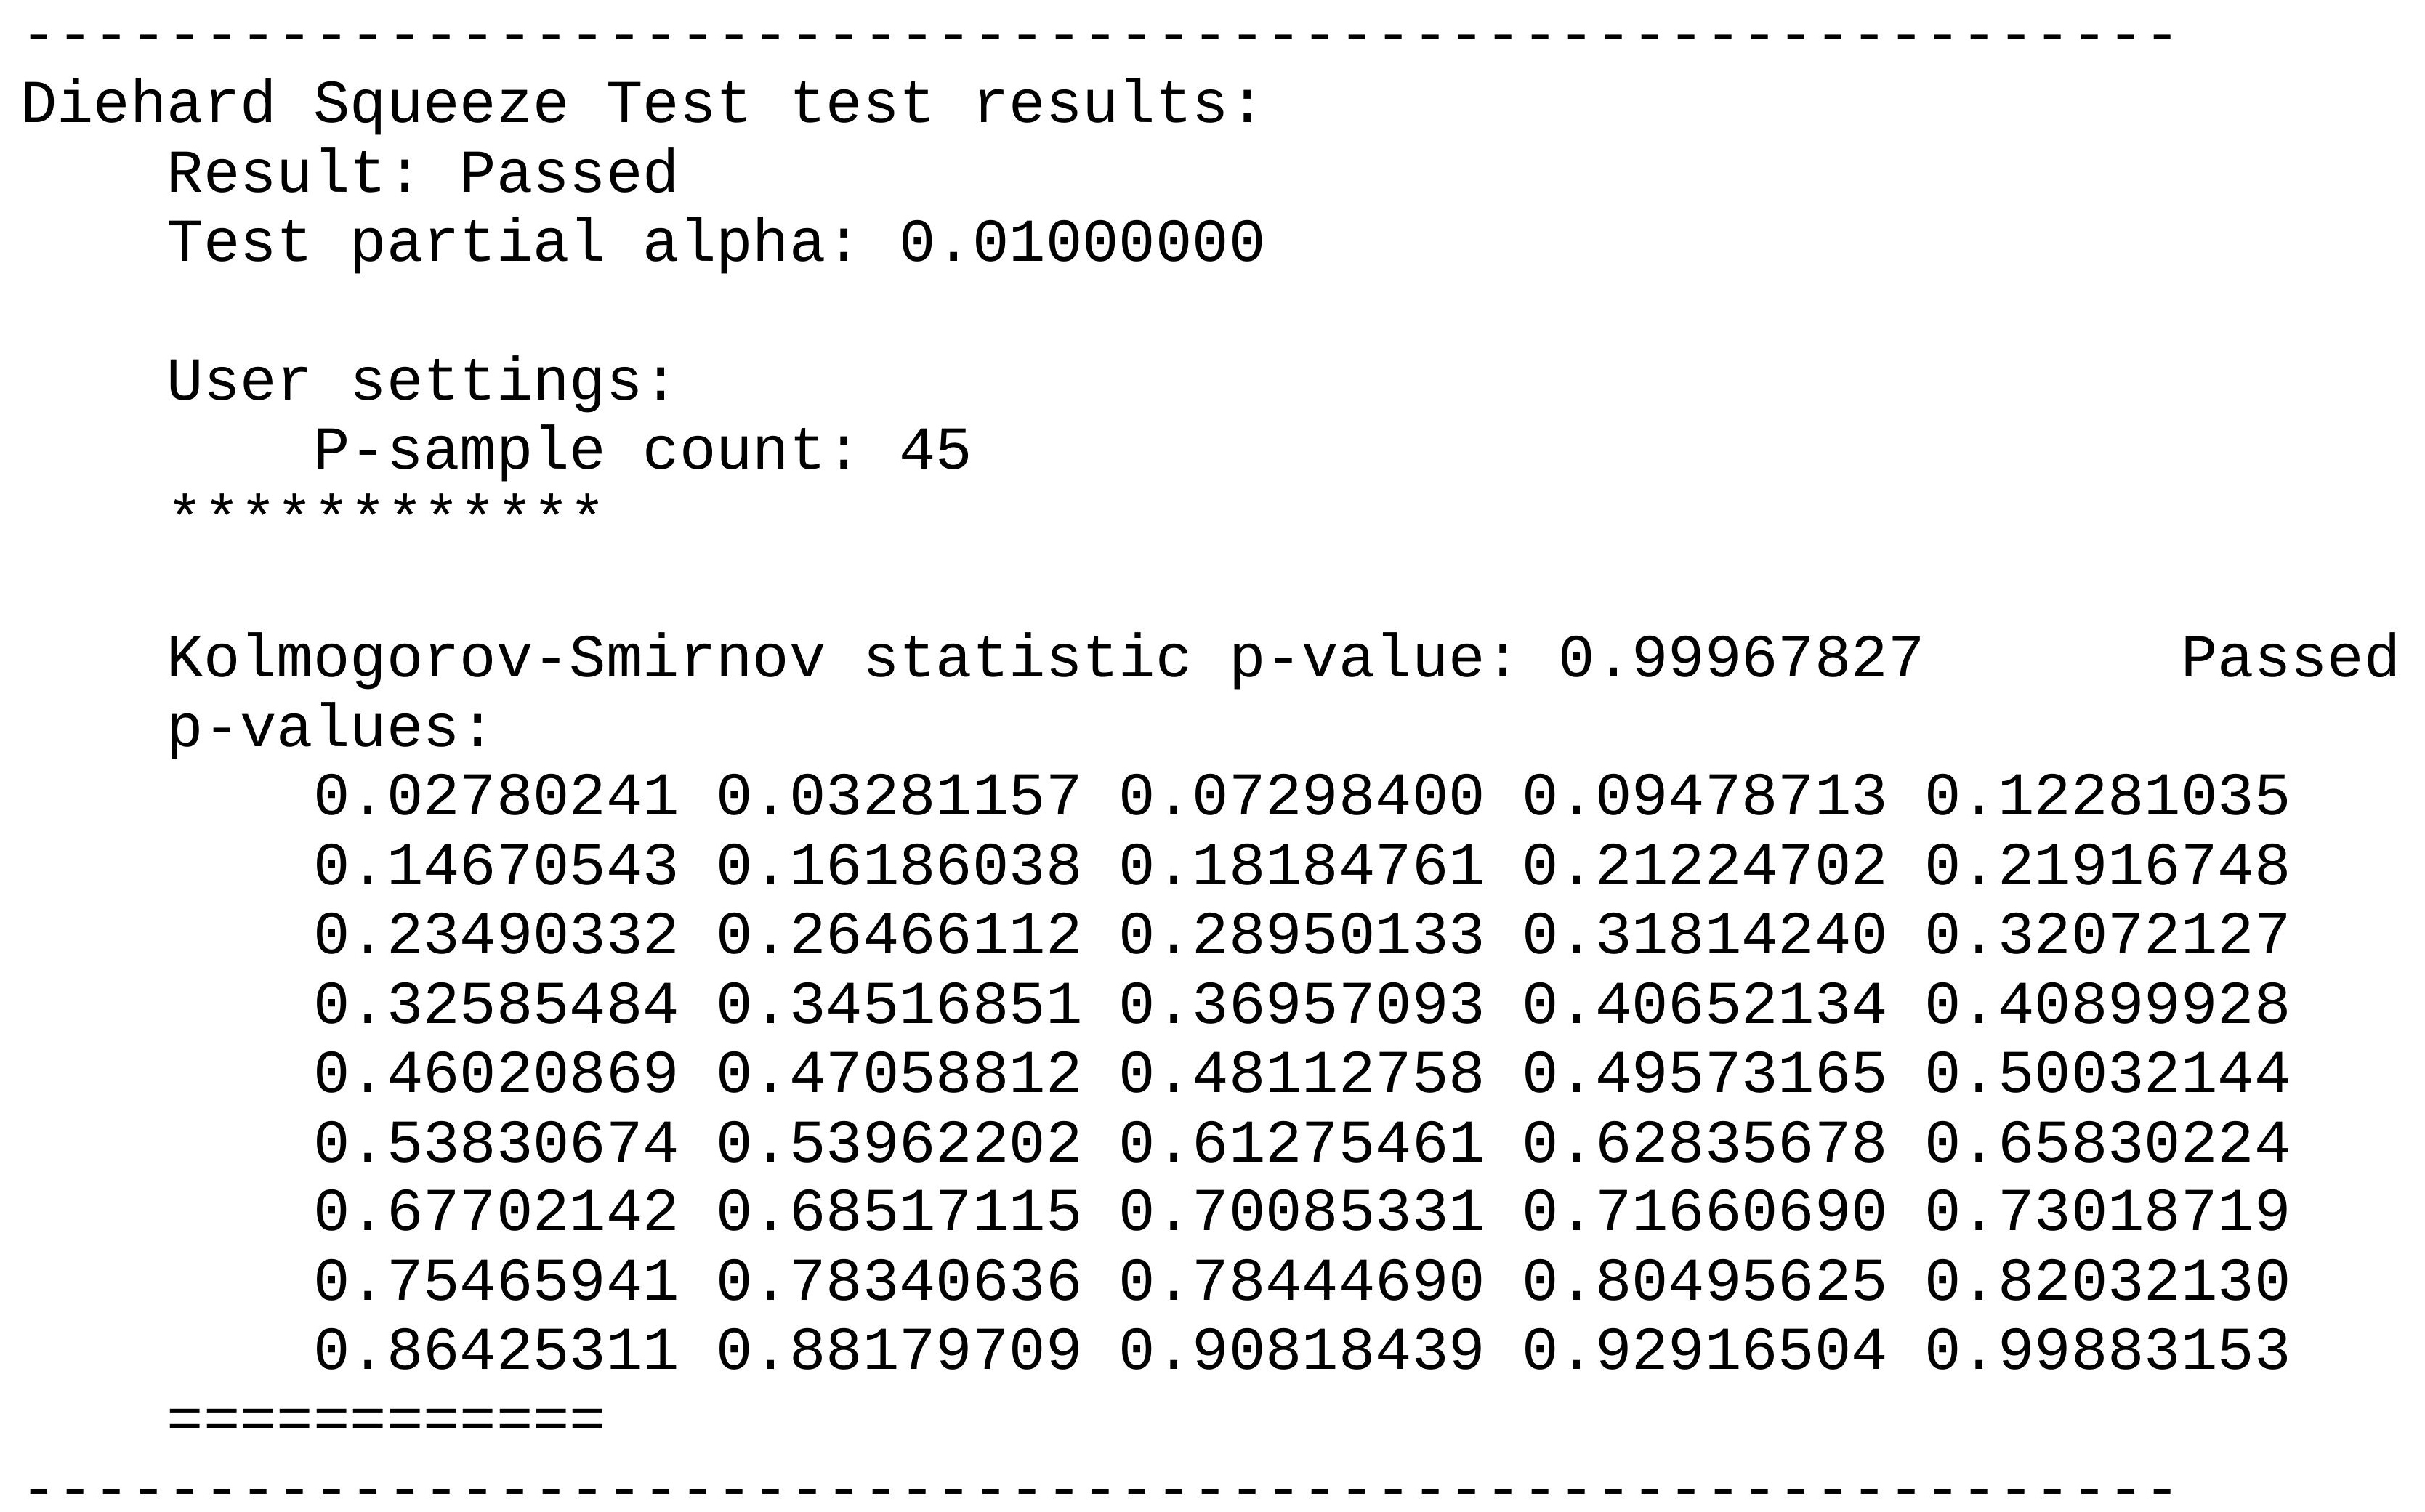
\includegraphics[width=12cm]{figures/rtt_dieharder_output.jpg}
  \end{center}
  \caption{The example of an individual test report from the \emph{RTT}.}
  \label{fig:rtt_output_example}
\end{figure}


\subsection{Randomness Testing Toolking in Python} \label{chap:sols-rtt-py}
The Randomness Testing Toolkit in Python (\emph{rtt-py}) was created by Patrik Vaverčák. It is supposed to be an improved version of \emph{RTT} sharing the same concept \cite[p.~24]{vavercak} and it was written in Python.

The included batteries are Dieharder, NIST STS, FIPS, and BSI. From TestU01, the \emph{rtt-py} also includes Rabbit, Alphabit, and BlockAlphabit batteries. The \emph{Crush} family batteries are not run, even though arguments of \emph{rtt-py} suggest that they are included. The \emph{rtt-py} allows for multiple files to be tested at once.

The \emph{rtt-py} is available at GitHub \cite{rtt-py-site} and implementations of all used batteries are in a single GitHub repository \cite{rtt-py-batteries}. Before running, both the \emph{rtt-py} and the batteries have to be installed as described in the project's README.

\subsubsection{Settings of \emph{rtt-py}}
The settings of \emph{rtt-py} use the same format as the original \emph{RTT} (as described in Subsection \ref{chap:sols-rtt}). The \emph{general settings} from the \emph{RTT} should be compatible with \emph{rtt-py} (although not the other way around) \cite[p. 25]{vavercak}. In reality, there is a problem with settings for the NIST STS's experiments directory. Also, no database connection is implemented in \emph{rtt-py}, therefore the \emph{mysql-db} attribute is ignored \cite{rtt-py-site}.

The second part of user settings are the battery configurations. They use the same format as in \emph{RTT} (as described in \ref{rtt-settings}) and are interchangeable \cite[p.~25]{vavercak}. The user has to keep in mind that the \emph{rtt-py} uses FIPS and BSI batteries, which are not used in \emph{RTT}. 

\subsubsection{Output \emph{rtt-py}}
The \emph{rtt-py} creates output in two formats -- \emph{CSV}\footnote{Comma-Separated values} and \emph{HTML}\footnote{HyperText Markup Language} \cite[p.~36]{vavercak}. Both of these report formats contain overview table. Each row from the table represents result of one individual test or subtest. The first column contains the name of the test and the name of the battery it belongs to. The second column contains \emph{failure rate} -- the ratio of tested files not passing the first-level test.

Each of the following columns is named after one tested file. The record contains either the second-level p-value reported by the test or the number of failed runs -- this depends on the battery. An example of this table can be seen in Figure \ref{fig:rtt_py_table}.

\begin{figure}
  \begin{center}
    %% minimus is about 100 pixels per 1 centimeter or 300 pixels per 1 inch.
    %% The optimum is about 250 pixels per 1 centimeter 
    \frame{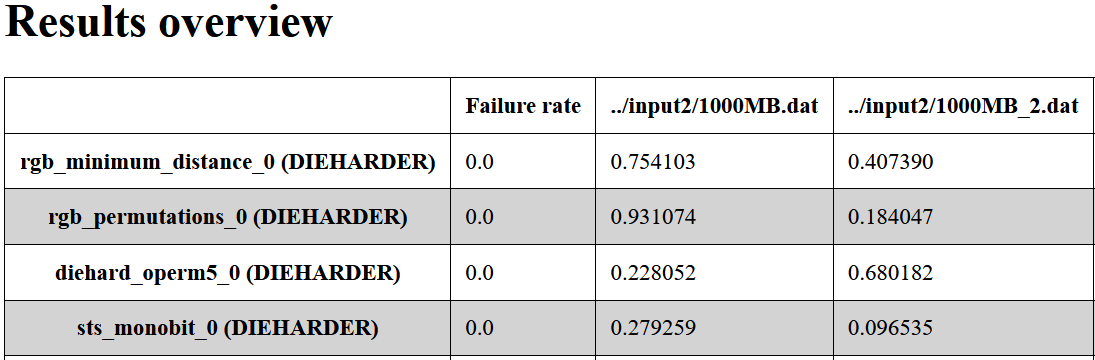
\includegraphics[width=12.5cm]{figures/rtt-py-table2.png}}
  \end{center}
  \caption{The example of the overview table from the \emph{rtt-py}}
  \label{fig:rtt_py_table}
\end{figure}


The output in the HTML format reports more information compared to the output in the CSV format. For each battery and for each tested file an HTML file with reports is generated.

In the report file there is a list of reports for each individual test or subtest from the given battery containing the result (either reported p-value, or number of failed runs). The individual test has a red background in case the test \emph{rejected} the null-hypothesis, grey background otherwise. It may contain additional information such as settings of the test or other information connected to the result, depending on the battery and the executed test. An example of the  report can be seen in Figure \ref{fig:rtt_py_html}
\begin{figure}
  \begin{center}
    %% minimus is about 100 pixels per 1 centimeter or 300 pixels per 1 inch.
    %% The optimum is about 250 pixels per 1 centimeter 
    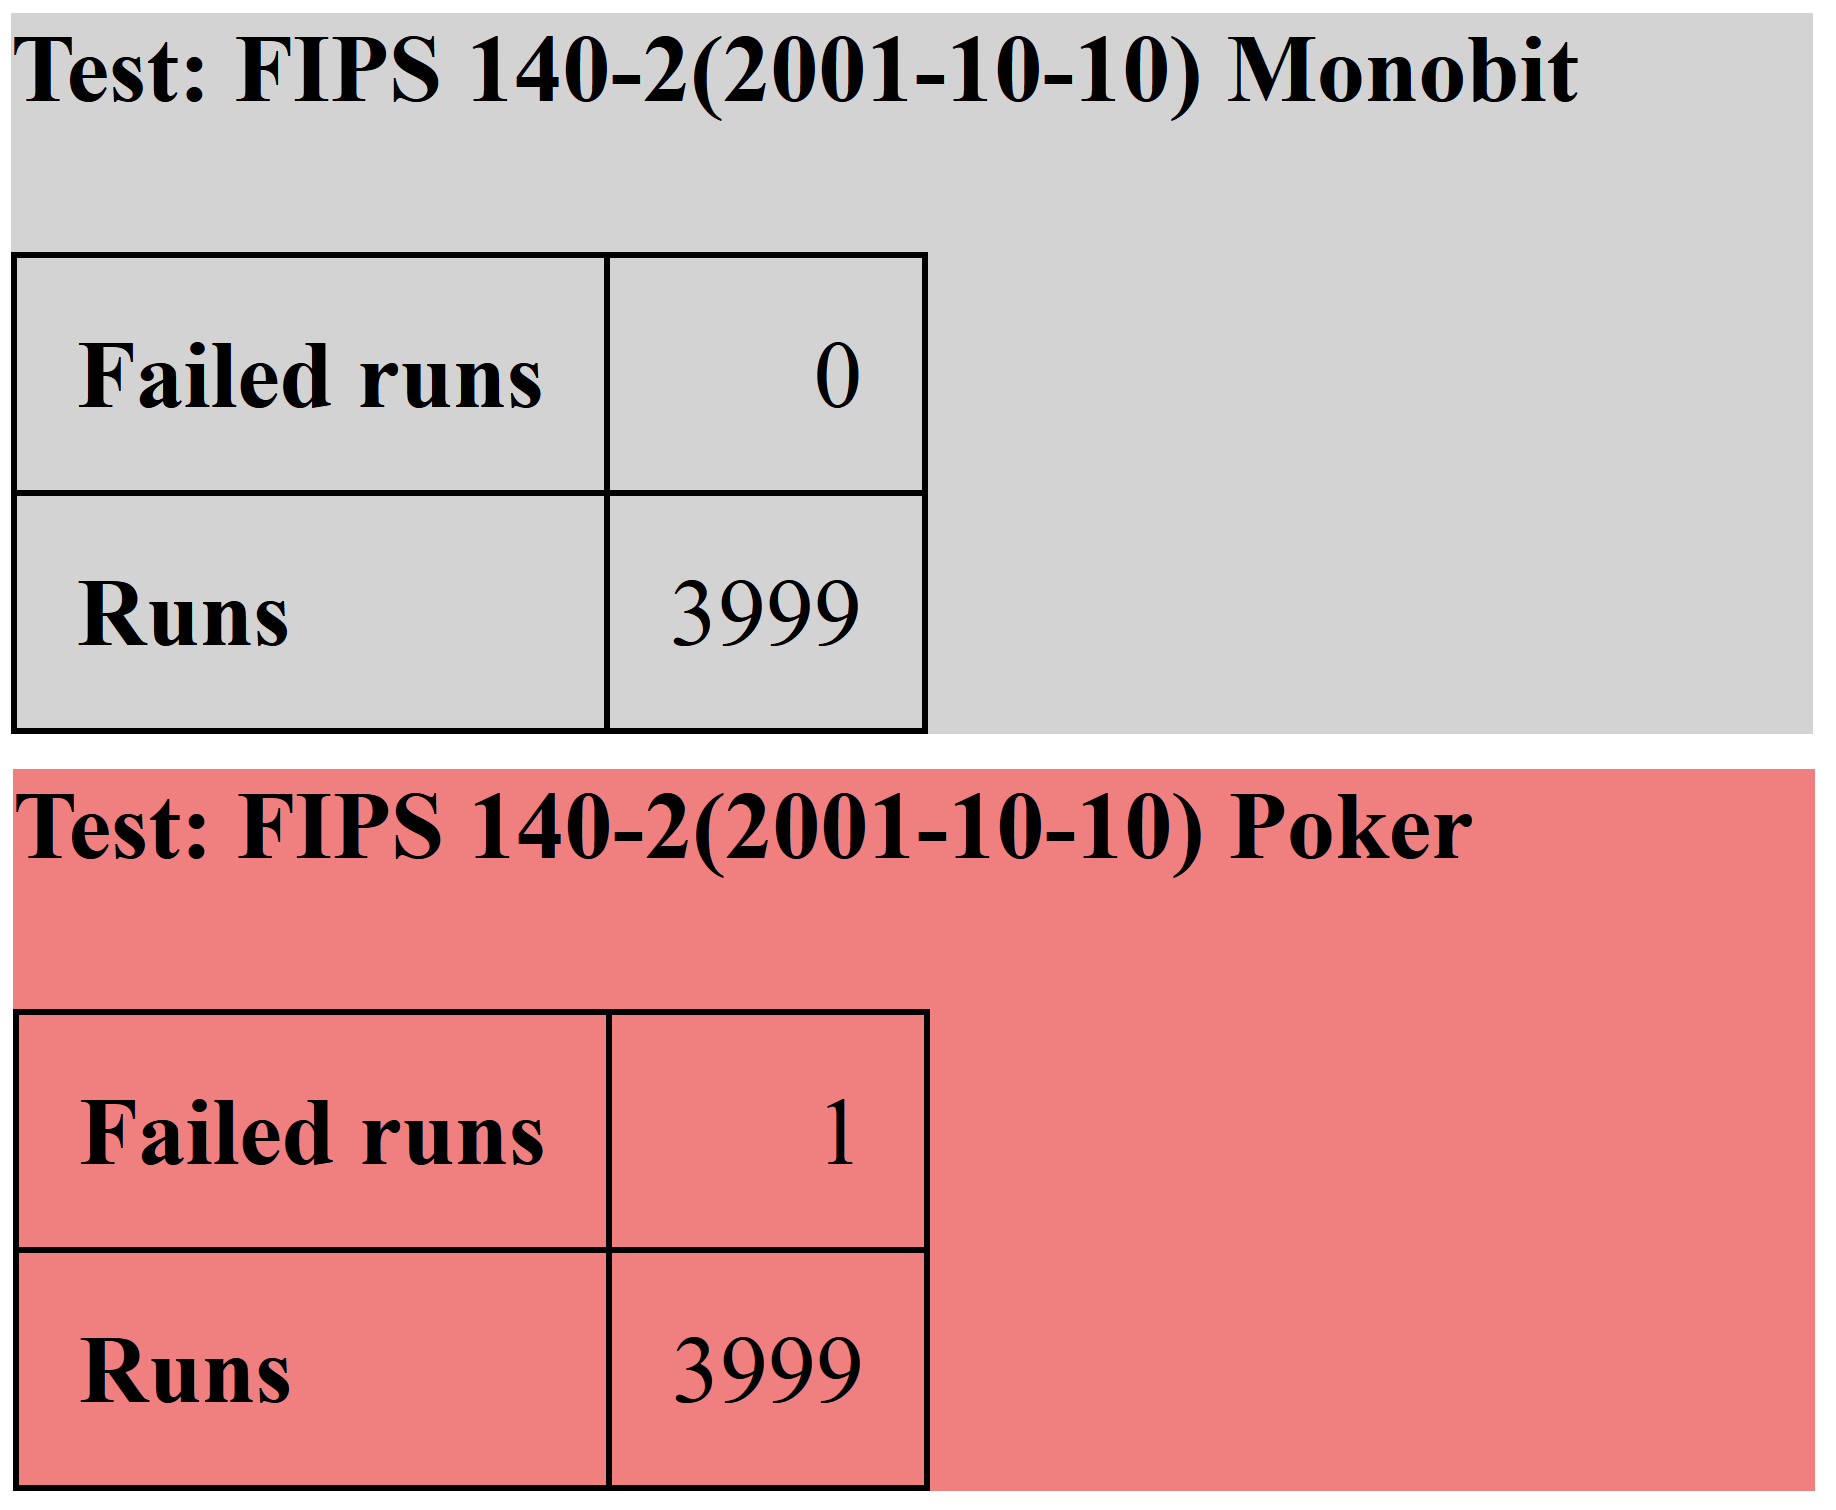
\includegraphics[width=12.5cm]{figures/rtt-py.png}
  \end{center}
  \caption{The example of HTML FIPS battery report from the \emph{rtt-py}.}
  \label{fig:rtt_py_html}
\end{figure}




% TEST ANALYSIS

\chapter{Tests Analysis} \label{chap: analysis}
This chapter aims to provide more information about the tests from the practical point of view. First, we analysed how much data the tests use to help with configurations of the batteries. Next, we measured how much time each test from the batteries takes to run. Data from both parts were used to create a program for automatic creation of test configurations for \emph{RTT} and \emph{rtt-py} -- the \emph{Configuration Calculator}. In the last section, we present a problem with non-uniform distributions of first-level p-values.
% is aimed at finding tests with problematic (non-uniform) distributions.


%%%%%%%%%%%%%%%%%%%
% DATA CONSUMPTION
%%%%%%%%%%%%%%%%%%%
%Dieharder X
%Nist - Omit
%Rabbit - to finish
%SmallCrush - X
%Crush - X
%Block(Alphabit) - omit


\section{Data Consumption} \label{chap:analysis-data}
%several big tables, mention exact parameters the tests  were run with

% configurable x fixed size
% variable x constant
As mentioned in Subsection \ref{chap:sols-batteries}, an important part of preventing \emph{file rewinds} is correct configuration of the tests. This is a complicated task because the user has to know the size of test first-level subsequences. To help with this task, I performed an analysis of first-level subsequence sizes for Dieharder, SmallCrush, Crush and Rabbit batteries.  

The NIST STS, Alphabit and BlockAlphabit batteries are not shown because the first-level subsequence size is set by the user. Unlike in the Rabbit battery, the tests from the mentioned batteries were observed to use the amount of data specified by their arguments. The BigCrush battery was skipped because its first-level subsequence sizes are larger than the currently intended use of RTT.


% INTRODUCTION
\subsection{Prelude} \label{chap:analysis-data-intro}
The idea was to run all tests from the batteries and calculate how many bytes were used for each individual test or test variant based on data provided by the batteries. Based on this information, a table for each battery containing this information was created.

The tests are divided into categories based on two properties. The first property is user's influence on the first-level subseqeunce size. Second property is if \emph{all} runs of the \emph{same} first-level tests use \emph{equal} size of first-level subsequence, or if the first-level subseqeunce size is different for each run. 

In the subsequent text, I use the following terminology. Based on the first property, the tests are called as:
\begin{markdown*}{%
  hybrid,
  definitionLists,
  footnotes,
  inlineFootnotes,
  hashEnumerators,
  fencedCode,
  citations,
  citationNbsps,
  pipeTables,
  tableCaptions,
}
* \emph{Tests with configurable size} are the tests where the size of first-level subsequence can be set by the user.
* \emph{Tests with fixed size} have predefined and unchangeable first-level subsequence size.
\end{markdown*}
Based on the second property, the categories are called:
\begin{markdown*}{%
  hybrid,
  definitionLists,
  footnotes,
  inlineFootnotes,
  hashEnumerators,
  fencedCode,
  citations,
  citationNbsps,
  pipeTables,
  tableCaptions,
}

* \emph{Tests with constant size} are the tests where the first-level subsequence is equal for all runs.
* \emph{Tests with variable size} are the tests where the first-level subsequence size fluctuates.

\end{markdown*}

The size of the first-level subsequence in the tests with variable size is determined by \emph{content} of the sequence. 
For example, the Diehard Squeeze Test starts with number $k=2^{31}$ and finds $j$, the number of iterations needed to reduce $k$ to 1 using the reduction $k=\lceil k\cdot U \rceil $, $U$ is uniform float on $[0,1)$ generated from 4 bytes of the tested data.

For an \emph{individual} test from this category and for random content of the sequence, the \emph{real} size of the first-level sequence fluctuates around \emph{some} value. 

To examine how long are the first-level sequences of tests with variable size, we run each test from this category at least 100 times on different \emph{random} data (taken from \emph{/dev/random}). Tests from this category are presented in their own tables containing mean length of the subsequence and differences between mean and lowest and highest observed length.

To verify that tests with constant size are indeed constant, I run them several times with different number of first-level sequences. The table for them contains only length of the subsequence.



\subsection{Dieharder}

%args
% "../../../rtt-statistical-batteries-master/dieharder", "-f", input_file, "-S 0 -s 1", "-g 201", "-D 131180","-d {}".format(test_id), "-p 25" if test_id in {13, 16} else "-p 5"
In Dieharder both tests with configurable and fixed size are present. All tests with configurable size have a default setting for first-level sequence size, which is usually used. Therefore all tests from this battery are in the analysis viewed as tests with fixed size. The subsequence sizes are presented in three tables.

Table \ref{tab:analysis_dieharder_variable} contains tests with \emph{variable sizes}. The tests with \emph{constant} sizes are split in two tables. In Table \ref{tab:analysis_dieharder}, the tests with \emph{no variants} are shown, the tests \emph{with varints} are shown in Table \ref{tab:analysis_dieharder_variants}.


\begin{table}[H]
  \begin{tabularx}{0.72\textwidth}{lcr}
    {\begin{tabularx}{0.3\textwidth}{l|r}
        Test ID &  size\\
         &  (bytes)\\
        \midrule
        0 & 153,600\\
        1 & 4,000,020\\
        2 & 5,120,000\\
        3 & 2,400,000\\
        4 & 1,048,584\\
        5 & 8,388,608\\
        6 & 5,592,416\\
        7 & 2,621,484\\
        8 & 256,004\\
        9 & 5,120,000\\
        10 & 96,000\\
        11 & 64,000\\
    \end{tabularx}} 
    
    {\begin{tabularx}{0.1\textwidth}{cc}
      & \\
    \end{tabularx}} 

    {\begin{tabularx}{0.32\textwidth}{l|r}
        Test ID &  size\\
         &  (bytes)\\
        \midrule
        12 & 48,000\\
        14 & 796\\
        15 & 400,000\\
        17 & 80,000,000\\
        100 & 400,000\\
        101 & 400,000\\
        102 & 400,000\\
        204 & 40,000 \\
        205 & 614,400,000 \\ 
        206 & 51,200,000 \\
        209 & 260,000,000 \\ 
        &
        
    \end{tabularx}} 
  \end{tabularx}
  \caption{First-level subseqeunces sizes for Dieharder tests with \emph{constant} sizes and no test variants.}
  \label{tab:analysis_dieharder}
\end{table}


\begin{table}[h]
  \begin{tabularx}{0.7\textwidth}{c|r|c|c}
    %\toprule
    Test ID & mean size & $\Delta$ min size & $\Delta$ max size\\
     & (bytes) & & \\
    \midrule
    13 & 9,225,521 & 0.039\% & 0.038\%\\
    16 & 5,402,335 & 0.126\% & 0.077\%\\
    207 & 452,016,414 & 0.019\% & 0.015\%\\
    208 & 116,881,517 & 0.047\% & 0.014\%\\
 
  \end{tabularx}
  \caption{First-level subseqeunce sizes for Dieharder tests with \emph{variable} sizes.}
  \label{tab:analysis_dieharder_variable}
\end{table}

\newpage

\begin{table}[H]
  \begin{tabularx}{\textwidth}{lcr}
    {\begin{tabularx}{0.35\textwidth}{lr|r}
        ID & ntup & size\\
        & & (bytes)\\
        \midrule
    200 & 1 & 800,004\\
    200 & 2 & 1,600,004\\
    200 & 3 & 2,400,004\\
    200 & 4 & 3,200,004\\
    200 & 5 & 4,000,004\\
    200 & 6 & 4,800,004\\
    200 & 7 & 5,600,004\\
    200 & 8 & 6,400,004\\
    200 & 9 & 7,200,004\\
    200 & 10 & 8,000,004\\
    200 & 11 & 8,800,004\\
    200 & 12 & 9,600,004\\
    201 & 2 & 80,000\\
    201 & 3 & 120,000\\
    201 & 4 & 160,000\\
    201 & 5 & 200,000\\
    202 & 2 & 800,000\\
    202 & 3 & 1,200,000\\
    202 & 4 & 1,600,000\\
    202 & 5 & 2,000,000 \\ 
    203 & 0 & 4,000,000 \\ 
    203 & 1 & 8,000,000 \\
    203 & 2 & 12,000,000 \\ 
    203 & 3 & 16,000,000 \\
    203 & 4 & 20,000,000 \\
    203 & 5 & 24,000,000 \\
    203 & 6 & 28,000,000 \\
    \end{tabularx}} 
    {\begin{tabularx}{0.1\textwidth}{cc}
      & \\
    \end{tabularx}} 

    {\begin{tabularx}{0.35\textwidth}{lr|r}
        ID & ntup & size\\
        & & (bytes)\\
        \midrule
        203 & 7 & 32,000,000 \\
        203 & 8 & 36,000,000 \\
        203 & 9 & 40,000,000 \\
        203 & 10 & 44,000,000 \\ 
        203 & 11 & 48,000,000 \\
        203 & 12 & 52,000,000 \\
        203 & 13 & 56,000,000 \\
        203 & 14 & 60,000,000 \\
        203 & 15 & 64,000,000 \\
        203 & 16 & 68,000,000 \\
        203 & 17 & 72,000,000 \\
        203 & 18 & 76,000,000 \\
        203 & 19 & 80,000,000 \\
        203 & 20 & 84,000,000 \\
        203 & 21 & 88,000,000 \\
        203 & 22 & 92,000,000 \\
        203 & 23 & 96,000,000 \\
        203 & 24 & 100,000,000 \\ 
        203 & 25 & 104,000,000 \\
        203 & 26 & 108,000,000 \\
        203 & 27 & 112,000,000 \\
        203 & 28 & 116,000,000 \\
        203 & 29 & 120,000,000 \\
        203 & 30 & 124,000,000 \\
        203 & 31 & 128,000,000 \\
        203 & 32 & 132,000,000 \\
            &    &
    \end{tabularx}} 
  \end{tabularx}
  \caption{First-level subseqeunce sizes for Dieharder tests with \emph{constant} sizes and test variants.}
  \label{tab:analysis_dieharder_variants}
\end{table}

\newpage


\subsection{TestU01 SmallCrush and Crush}
In the SmallCrush and Crush batteries, only tests with \emph{fixed} size are present. Both batteries contain tests with \emph{variable} size, which are shown in Table \ref{tab:analysis_smallcrush_variable} for SmallCrush and in Table \ref{tab:analysis_crush_variable} for Crush. The tests with \emph{constant} sizes from SmallCrush are in Table \ref{tab:analysis_smallcrush}, from Crush in  Table \ref{tab:analysis_crush}.


\begin{table}[h]
  \begin{tabularx}{0.75\textwidth}{c|r|r|r}
    %\toprule
   Test ID & mean size & $\Delta$ min size & $\Delta$ max size\\
     & (bytes) & & \\
     \midrule
    3 & 204,733,510 & 0.563\% & 0.725\% \\
    5 & 98,731,035 & 0.095\% & 0.087\% \\
  \end{tabularx}
  \caption{First-level subseqeunce sizes for \emph{SmallCrush} tests with \emph{variable} sizes.}
  \label{tab:analysis_smallcrush_variable}
\end{table}

\begin{table}[h]
  \begin{tabularx}{0.36\textwidth}{c|r}
  Test ID & size \\
    & (bytes) \\
  \midrule
    1 & 40,000,000 \\
    2 & 40,000,000 \\
    4 & 102,400,000 \\
    6 & 48,000,000 \\
    7 & 204,800,000 \\
    8 & 28,800,000 \\
    9 & 120,000,000 \\
    10 & 20,000,000 \\

  \end{tabularx}
  \caption{First-level subseqeunce sizes for \emph{SmallCrush} tests with \emph{constant} sizes.}
  \label{tab:analysis_smallcrush}
\end{table}

\begin{table}[h]
  \begin{tabularx}{0.75\textwidth}{c|r|r|r}
    %\toprule
   Test ID & mean size & $\Delta$ min size & $\Delta$ max size\\
     & (bytes) & & \\
    \midrule
    27&1,333,326,306&0.0163\%&0.0166\%\\
    28&1,333,331,101&0.0188\%&0.0170\%\\	
    29&1,974,653,548&0.0189\%&0.0196\%	\\
    30&1,974,640,110&0.0164\%&0.0146\%	\\
    31&3,200,051,704&0.0204\%&0.0306\%	\\
    32&3,199,995,653&0.0380\%&0.0244\%	\\
    33&5,120,635,483&0.1408\%&0.1618\%	\\
    34&5,119,635,549&0.1399\%&0.2516\%	\\
    55&1,653,334,290&0.0065\%&0.0060\%	\\
    64&320,000,610&5.31$\cdot10^{-5}$\% &4.43$\cdot10^{-5}$\%\\
    91&533,332,642&0.0039\%&0.0037\%	\\
    92&1,599,996,811&0.0049\%&0.0043\%\\

  \end{tabularx}
  \caption{First-level subseqeunce sizes for \emph{Crush} tests with \emph{variable} sizes.}
  \label{tab:analysis_crush_variable}
\end{table}

% LONGTABLE
\begin{longtable}[c]{l|rcl|r}

\caption{First-level subseqeunce sizes for \emph{Crush} tests with \emph{constant} sizes. \label{tab:analysis_crush}}\\
 \hline
 \multicolumn{5}{| c |}{Begin of Table}\\
 \hline
 
 Test ID & size & & Test ID & size \\
  & (bytes) & & &  (bytes)\\
 \cline{1-2} \cline{4-5}
 \endfirsthead

 \hline
 \multicolumn{5}{|c|}{Continuation of Table \ref{tab:analysis_crush}}\\
 \hline
 Test ID & size & & Test ID & size \\
  & (bytes) & & &  (bytes)\\
 \cline{1-2} \cline{4-5}
 \endhead

 \hline
 \endfoot

 \hline
 \multicolumn{5}{| c |}{End of Table}\\
 \hline\hline
 \endlastfoot
1 & 2,000,000,000 &  & 52 & 2,048,000,000\\
2 & 1,200,000,000 &  & 53 & 2,048,000,000\\
3 & 400,000,000 &  & 54 & 2,048,000,000\\
4 & 400,000,000 &  & 56 & 480,000,000\\
5 & 400,000,000 &  & 57 & 1,440,000,000\\
6 & 400,000,000 &  & 58 & 600,000,000\\
7 & 400,000,000 &  & 59 & 1,800,000,000\\
8 & 400,000,000 &  & 60 & 384,000,000\\
9 & 400,000,000 &  & 61 & 1,152,000,000\\
10 & 400,000,000 &  & 62 & 2,400,000,000\\
11 & 800,000,000 &  & 63 & 800,000,000\\
12 & 1,200,000,000 &  & 65 & 600,000,000\\
13 & 1,600,000,000 &  & 66 & 360,000,000\\
14 & 1,680,000,000 &  & 67 & 680,000,000\\
15 & 1,680,000,000 &  & 68 & 400,000,000\\
16 & 1,920,000,000 &  & 69 & 668,000,000\\
17 & 1,920,000,000 &  & 70 & 400,000,000\\
18 & 160,000,000 &  & 71 & 480\\
19 & 240,000,000 &  & 72 & 480\\
20 & 280,000,000 &  & 73 & 44,739,280\\
21 & 128,000,000 &  & 74 & 109,400,000\\
22 & 128,000,000 &  & 75 & 327,800,000\\
23 & 2,560,000,000 &  & 76 & 1,333,336,000\\
24 & 2,560,000,000 &  & 77 & 1,200,002,400\\
25 & 2,560,000,000 &  & 78 & 1,200,000,000\\
26 & 2,560,000,000 &  & 79 & 1,200,000,000\\
35 & 2,000,000,000 &  & 80 & 1,333,360,000\\
36 & 2,000,000,000 &  & 81 & 1,200,000,000\\
37 & 2,000,000,000 &  & 82 & 2,000,000,000\\
38 & 2,000,000,000 &  & 83 & 2,000,000,000\\
39 & 2,600,000,000 &  & 84 & 1,600,000,000\\
40 & 2,600,000,000 &  & 85 & 2,400,000,000\\
41 & 2,000,000,000 &  & 86 & 2,400,000,000\\
42 & 2,000,000,000 &  & 87 & 2,400,000,000\\
43 & 800,000,000 &  & 88 & 2,400,000,000\\
44 & 1,200,000,000 &  & 89 & 3,200,000,000\\
45 & 400,000,000 &  & 90 & 960,000,000\\
46 & 1,200,000,000 &  & 91 & 533,332,642\\
47 & 800,000,000 &  & 92 & 1,599,996,811\\
48 & 2,000,000,000 &  & 93 & 1,333,333,400\\
49 & 820,000,000 &  & 94 & 2,000,000,020\\
50 & 880,000,000 &  & 95 & 1,333,333,400\\
51 & 2,048,000,000 &  & 96 & 2,000,000,040\\

 \end{longtable}




% several tables, at least table for minims
\subsection{TestU01 Rabbit} \label{chap:analysis-data-rabbit}
All tests in the Rabbit battery are with \emph{configurable} size. The size is configured using the \emph{bit\textunderscore nb} argument, where the desired size is entered in \emph{bits} and for use is rounded down to closest multiple of 32. The \emph{bit\textunderscore nb} has no default value, must be at least 500 and \emph{at most} \emph{bit\textunderscore nb} bits will be read from the file. \cite[p. 152]{tu01_guide} However, almost half of the tests require bigger \emph{bit\textunderscore nb} and will not run otherwise. These tests and their required sizes are in Table \ref{tab:analysis_rabbit_minims}. The minimums were found and verified experimentally.

\begin{table}[h]
  \begin{tabularx}{0.4\textwidth}{c|r}
    %\toprule
    Test ID & minimal \emph{bit\textunderscore nb}\\
    \midrule
    9& 31,200\\
    10& 960\\
    11& 960\\
    15& 960\\
    16& 1,920\\
    17& 3,840\\
    21& 51,200\\
    22& 5,120,000\\
    23& 52,428,800\\
    24& 960\\
    25& 30,720\\
    26& 300,480\\
  \end{tabularx}
  \caption{Minimal values of \emph{bit\textunderscore nb} argument other than default needed to run tests from \emph{Rabbit} battery.}
  \label{tab:analysis_rabbit_minims}
\end{table}

Tests 6, 7 and 8 read only data with size $2^k$($k \in \mathbb{N}$) \emph{bits}. The possible values of $k$ are different for each test and shown in Table \ref{tab:analysis_rabbit_two_powers}. \cite[p.~124-126]{tu01_guide} If the \emph{bit\textunderscore nb} is not power of two, closest lower applicable power of 2 is used. The \emph{bit\textunderscore nb} still has to be at least 500, even though smaller amount of bits may be used.

\begin{table}[h]
  \begin{tabularx}{0.33\textwidth}{c|c}
    %\toprule
    Test ID & maximal $k$\\
    \midrule
    6& 28\\
    7& 20\\
    8& 26\\
 
  \end{tabularx}
  \caption{Maximal values of $k$ for Rabbit tests which take data of size $2^k$ \emph{bits}.}
  \label{tab:analysis_rabbit_two_powers}
\end{table}

The only test with \emph{variable} size from Rabbit battery is the test 20. It uses around 80 \% of the data size specified by \emph{bit\textunderscore nb} argument. Test 5 reads significantly less data than specified. When the \emph{bit\textunderscore nb} argument specifies that the test should use 10MB of data, the test 5 uses only  3,536 \emph{bytes}. When the test should use 100MB of data, it uses only 8,488 \emph{bytes}.

For some tests with \emph{constant} size, there is an \emph{upper bound} of data used for testing. The test will not read more data than this value, even when specified by the \emph{bit\textunderscore nb} argument. The size of data that are actually read from the file is different for each value of \emph{bit\textunderscore nb} greater than the \emph{upper bound} and fluctuates around \emph{some} value. Examples of real data size fluctuation are in the Figure \ref{fig:analysis-rabbit-max}.

\begin{figure}[h]
  \begin{center}
    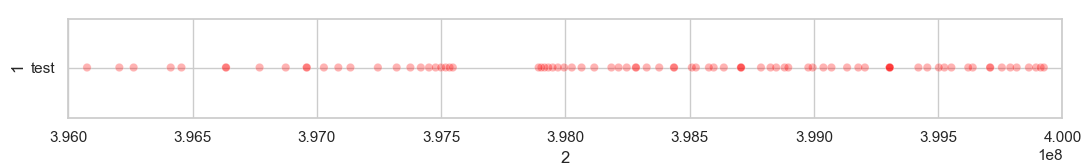
\includegraphics[width=12.7cm]{figures/rabbit_3_maxims.png}
  \end{center}
  \caption{Number of bytes actually read from tested file by Rabbit test with ID 3 for various values of \emph{bit\textunderscore nb} greater than 3.3$\cdot10^{9}$ ($\approx$~393~megabytes).}
  \label{fig:analysis-rabbit-max}
\end{figure}
%For the following analysis of first-level subseqeunce sizes the \emph{bit\textunderscore nb} argument was fixed to value 52,428,800. This is the lowest value for which all tests from Rabbit, Alphabit and BlockAlphabit will run (all batteries from TestU01 using \emph{bit\textunderscore nb} argument).

%TODO: upper bound

%%%%%%%%%%%%%%%%%%%
% Time consumption
%%%%%%%%%%%%%%%%%%%

% Dieharder X 
% Nist X
% SmallCrush X
% Crush X
% Rabbit X
% Alphabit X

\section{Time consumption and performance} \label{chap:analysis-times}
%again some big tables, choose one test as a reference and the rest will be relative. mention exact parameters, maybe add throughput?


Another analysis we performed is examination of the tests' runtimes and performance. This may be used to \emph{exempt} tests that would take \emph{unreasonably} long to execute or to detect problems while running the tests (for example when the test execution gets stuck on non-random data).

Because the runtimes highly depend on used machine and the idea is to make relative comparison between the tests only, they are presented in \emph{relative} form compared to the runtime of Diehard 3d Sphere (Minimum Distance) Test from Dieharder battery (later refered to as \emph{time unit} or \emph{TU}).\footnote{Running on Intel Core i7-1065G7 CPU under Ubuntu 22.04.1 WSL on Windows~10 this test took 0.021 seconds.} 

To compare performance of the tests, \emph{throughput} was chosen as a measure. It is presented alongside the runtime. The throughput is calculated as kilobytes\footnote{1024 bytes} of data processed per time unit. 

The used implementations of batteries are taken from RTT (available from \cite{rtt-batteries}). The batteries were run directly (i.e. not using RTT) and each individual test was executed in separate at least one hundred times. Mean runtime over these runs is presented in this Section.

The runtimes and throughputs for Dieharder are in Table \ref{tab:analysis_time_dieharder}. The Dieharder tests were run without the \emph{rate} option and with default values of \emph{tsample} argument. Runtimes and throughputs for TestU01 SmallCrush and Crush batteries are in Table \ref{tab:analysis_smallcrush_time} and Table \ref{tab:analysis_crush_times}.

To measure runtimes of test with \emph{configurable} size, I had to fix the first-level subsequence size for each test. For NIST STS battery, I set \emph{stream size} argument to 1,000,000 (the subsequences were 125,000  bytes long). This is the lowest value which satisfies subsequence size recommendations for all the tests. \cite{nist_special} NIST STS runtimes and throughputs are shown in Table \ref{tab:analysis_nist_time}.

For TestU01 Rabbit, Alphabit and BlockAlphabit batteries, I fixed the \emph{bit\textunderscore nb} argument to value 52,428,800 (the subseqeunces should be 6,553,600 bytes long). This is the lowest value for which all tests from the three batteries are executed (see Subsection \ref{chap:analysis-data-rabbit}). The runtimes and throughputs for Rabbit battery are in Table \ref{tab:analysis_rabbit_time}. Alphabit and BlockAlphabit batteries share Table \ref{tab:analysis_alphabit_time}, because both batteries employ the \emph{same} tests and no difference in runtimes was observed.

\begin{table}[H]
  \begin{tabularx}{1\textwidth}{lcr}
    {\begin{tabularx}{0.43\textwidth}{c|r|r}
        ID & runtime & Throughput\\
         & (TU) & (kB/TU) \\
        \midrule
        0 & 0.43 & 347 \\
        1 & 2.93 & 1332 \\
        2 & 9.28 & 539 \\
        3 & 2.10 & 1116 \\
        4 & 0.91 & 1126 \\
        5 & 4.79 & 1710 \\
        6 & 33.36 & 164 \\
        7 & 10.01 & 256 \\
        8 & 0.21 & 1208 \\
        9 & 2.86 & 1751 \\
        10 & 0.73 & 128 \\
        11 & 0.27 & 236 \\
        12 & 1.00 & 47 \\
        13 & 5.70 & 1581 \\
    \end{tabularx}} 
    {\begin{tabularx}{0.1\textwidth}{cc}
      & \\
    \end{tabularx}} 

    {\begin{tabularx}{0.43\textwidth}{c|r|r}
        ID & runtime & Throughput\\
         & (TU) & (kB/TU) \\
        \midrule 
        14 & 3.03$\cdot10^{-5}$ & 25598 \\
        15 & 0.25 & 1585 \\
        16 & 2.86 & 1846 \\
        17 & 75.79 & 1031 \\
        100 & 0.19 & 2024 \\
        101 & 2.73 & 143 \\
        102 & 4.29 & 91 \\
        204 & 0.06 & 604 \\
        205 & 311.59 & 1926 \\
        206 & 44.78 & 1117 \\
        207 & 272.13 & 1622 \\
        208 & 180.61 & 632 \\
        209 & 266.52 & 953 \\
         & &\\

    \end{tabularx}} 
  \end{tabularx}
  \caption{Runtimes for and throughputs Dieharder battery tests without variants.}
  \label{tab:analysis_time_dieharder}
\end{table}

\begin{table}[H]
  \begin{tabularx}{1\textwidth}{lr}
    {\begin{tabularx}{0.5\textwidth}{c|c|r|r}
        ID & ntup & runtime & Through\\
         & & & put \\
         & & (TU) & (kB/TU) \\
        \midrule
        200 & 1 & 1.18 & 662 \\
        200 & 2 & 1.59 & 983 \\
        200 & 3 & 1.89 & 1238 \\
        200 & 4 & 2.30 & 1359 \\
        200 & 5 & 3.02 & 1295 \\
        200 & 6 & 4.20 & 1116 \\
        200 & 7 & 5.98 & 915 \\
        200 & 8 & 7.06 & 885 \\
        200 & 9 & 8.90 & 790 \\
        200 & 10 & 11.40 & 685 \\
        200 & 11 & 15.90 & 540 \\
        200 & 12 & 24.84 & 377 \\
        201 & 2 & 0.28 & 279 \\
        201 & 3 & 0.34 & 347 \\
        201 & 4 & 0.50 & 310 \\
        201 & 5 & 0.87 & 225 \\
        202 & 2 & 0.47 & 1666 \\
        202 & 3 & 0.74 & 1590 \\
        202 & 4 & 1.09 & 1436 \\
        202 & 5 & 1.89 & 1033 \\
        203 & 0 & 2.00 & 1956 \\
        203 & 1 & 3.86 & 2025 \\
        203 & 2 & 5.88 & 1994 \\
        203 & 3 & 7.70 & 2030 \\
        203 & 4 & 9.90 & 1973 \\
        203 & 5 & 11.67 & 2009 \\
        203 & 6 & 13.63 & 2006 \\
    \end{tabularx}} 
    %{\begin{tabularx}{0.1\textwidth}{cc}
    %  & \\
    %\end{tabularx}} 

    {\begin{tabularx}{0.5\textwidth}{c|c|r|r}
       ID & ntup & runtime & Through\\
         & & & put \\
         & & (TU) & (kB/TU) \\
        \midrule 
        203 & 7 & 16.04 & 1948 \\
        203 & 8 & 17.64 & 1993 \\
        203 & 9 & 19.59 & 1994 \\
        203 & 10 & 21.24 & 2023 \\
        203 & 11 & 23.44 & 2000 \\
        203 & 12 & 25.24 & 2012 \\
        203 & 13 & 27.15 & 2014 \\
        203 & 14 & 29.19 & 2008 \\
        203 & 15 & 30.76 & 2032 \\
        203 & 16 & 32.89 & 2019 \\
        203 & 17 & 35.10 & 2003 \\
        203 & 18 & 36.79 & 2017 \\
        203 & 19 & 38.98 & 2004 \\
        203 & 20 & 40.36 & 2032 \\
        203 & 21 & 42.82 & 2007 \\
        203 & 22 & 44.86 & 2003 \\
        203 & 23 & 46.18 & 2030 \\
        203 & 24 & 49.11 & 1989 \\
        203 & 25 & 50.01 & 2031 \\
        203 & 26 & 51.24 & 2058 \\
        203 & 27 & 55.30 & 1978 \\
        203 & 28 & 57.85 & 1958 \\
        203 & 29 & 58.84 & 1992 \\
        203 & 30 & 61.32 & 1975 \\
        203 & 31 & 64.50 & 1938 \\
        203 & 32 & 65.41 & 1971 \\
         \\

    \end{tabularx}} 
  \end{tabularx}
  \caption{Runtimes and throughputs for Dieharder battery tests with variants.}
  \label{tab:analysis_time_dieharder_variants}
\end{table}



\begin{table}[H]
  \begin{tabularx}{0.5\textwidth}{c|r|r}
    %\toprule
    Test ID & runtime & throughput\\
     & (TU) & (kB/TU) \\
    \midrule
    1 & 0.16 & 782 \\
    2 & 0.17 & 716 \\
    3 & 0.16 & 765 \\
    4 & 0.19 & 658 \\
    5 & 0.17 & 711 \\
    6 & 0.24 & 500 \\
    7 & 5.79 & 21 \\
    8 & 0.77 & 158 \\
    9 & 0.20 & 597 \\
    10 & 0.22 & 560 \\
    11 & 0.22 & 561 \\
    12 & 0.43 & 283 \\
    13 & 0.39 & 314 \\
    14 & 0.93 & 132 \\
15 & 1.55 & 79 \\
  \end{tabularx}
  \caption{Runtimes and throughputs for NIST STS battery with \emph{stream size} 1,000,000 bits.}
  \label{tab:analysis_nist_time}
\end{table}


\begin{table}[H]
  \begin{tabularx}{0.5\textwidth}{c|r|r}
    Test ID & Runtime & Throughput\\
     & (TU) & (kB/TU) \\
    \midrule
    1 & 49.20 & 794 \\
    2 & 36.48 & 1071 \\
    3 & 16.21 & 12361 \\
    4 & 16.74 & 5973 \\
    5 & 13.03 & 7402 \\
    6 & 17.24 & 2719 \\
    7 & 12.94 & 15451 \\
    8 & 16.07 & 1750 \\
    9 & 22.76 & 5149 \\
    10 & 25.56 & 764 \\
  \end{tabularx}
  \caption{Runtimes and throughputs for TestU01 SmallCrush battery.}
  \label{tab:analysis_smallcrush_time}
\end{table}




\begin{longtable}[c]{c|r|rcc|r|r}
\caption{Runtimes and throughputs for TestU01 \emph{Crush} battery. \label{tab:analysis_crush_times}}\\
 \hline
 \multicolumn{7}{| c |}{Begin of Table}\\
 \hline
 Test ID & Runtime & Throughput & & Test ID & Runtime & Throughput \\
  & (TU) & (kB / TU) & & (TU) & (kB / TU)\\ 
 \cline{1-3} \cline{5-7}
 \endfirsthead

 \hline
 \multicolumn{7}{|c|}{Continuation of Table \ref{tab:analysis_crush_times}}\\
 \hline
 Test ID & Runtime & Throughput & & Test ID & Runtime & Throughput \\
  & (TU) & (kB / TU) & & (TU) & (kB / TU)\\ 
 \cline{1-3} \cline{5-7}
 \hline
 \endhead

 \hline
 \endfoot

 \hline
 \multicolumn{7}{| c |}{End of Table}\\
 \hline\hline
 \endlastfoot

 1 & 691.72 & 2824 &  & 49 & 239.32 & 3346\\
2 & 412.71 & 2839 &  & 50 & 82.72 & 10389\\
3 & 706.53 & 553 &  & 51 & 101.95 & 19618\\
4 & 744.61 & 525 &  & 52 & 131.29 & 15233\\
5 & 1001.45 & 390 &  & 53 & 147.27 & 13580\\
6 & 1014.13 & 385 &  & 54 & 152.78 & 13090\\
7 & 1046.35 & 373 &  & 55 & 109.68 & 14721\\
8 & 1033.21 & 378 &  & 56 & 770.92 & 608\\
9 & 995.59 & 392 &  & 57 & 808.59 & 1739\\
10 & 1005.83 & 388 &  & 58 & 1164.27 & 503\\
11 & 960.15 & 814 &  & 59 & 1379.70 & 1274\\
12 & 972.95 & 1204 &  & 60 & 1567.96 & 239\\
13 & 1001.15 & 1561 &  & 61 & 2014.98 & 558\\
14 & 644.60 & 2545 &  & 62 & 164.67 & 14233\\
15 & 675.67 & 2428 &  & 63 & 513.08 & 1523\\
16 & 651.24 & 2879 &  & 64 & 148.90 & 2099\\
17 & 644.66 & 2908 &  & 65 & 843.17 & 695\\
18 & 296.66 & 527 &  & 66 & 207.06 & 1698\\
19 & 408.85 & 573 &  & 67 & 682.89 & 972\\
20 & 763.62 & 358 &  & 68 & 177.12 & 2205\\
21 & 290.98 & 430 &  & 69 & 581.06 & 1123\\
22 & 249.12 & 502 &  & 70 & 157.27 & 2484\\
23 & 356.42 & 7014 &  & 71 & 522.24 & 1\\
24 & 418.57 & 5973 &  & 72 & 518.17 & 1\\
25 & 340.36 & 7345 &  & 73 & 632.92 & 69\\
26 & 414.22 & 6035 &  & 74 & 561.55 & 190\\
27 & 175.32 & 7427 &  & 75 & 599.53 & 534\\
28 & 210.22 & 6194 &  & 76 & 2024.52 & 643\\
29 & 217.71 & 8858 &  & 77 & 708.19 & 1655\\
30 & 256.83 & 7508 &  & 78 & 599.47 & 1955\\
31 & 227.35 & 13745 &  & 79 & 371.55 & 3154\\
32 & 288.64 & 10827 &  & 80 & 335.88 & 3877\\
33 & 249.16 & 20070 &  & 81 & 221.70 & 5286\\
34 & 310.39 & 16108 &  & 82 & 544.90 & 3584\\
35 & 210.76 & 9267 &  & 83 & 521.43 & 3746\\
36 & 277.00 & 7051 &  & 84 & 401.77 & 3889\\
37 & 685.43 & 2849 &  & 85 & 648.33 & 3615\\
38 & 694.09 & 2814 &  & 86 & 486.71 & 4815\\
39 & 1217.74 & 2085 &  & 87 & 642.08 & 3650\\
40 & 1261.90 & 2012 &  & 88 & 478.61 & 4897\\
41 & 802.82 & 2433 &  & 89 & 835.60 & 3740\\
42 & 474.13 & 4119 &  & 90 & 184.36 & 5085\\
43 & 115.48 & 6765 &  & 91 & 796.39 & 654\\
44 & 131.44 & 8916 &  & 92 & 952.65 & 1640\\
45 & 80.57 & 4848 &  & 93 & 540.12 & 2411\\
46 & 128.67 & 9108 &  & 94 & 659.61 & 2961\\
47 & 157.27 & 4968 &  & 95 & 447.90 & 2907\\
48 & 146.23 & 13356 &  & 96 & 527.98 & 3699\\

 \end{longtable}


 \begin{table}[H]
  \begin{tabularx}{0.5\textwidth}{c|r|r}
  Test ID & Runtime & Throughput \\
         & (TU) &  kb/TU\\
  \midrule
        1 & 3.49 & 1835 \\
        2 & 3.51 & 1825 \\
        3 & 3.36 & 1902 \\
        4 & 5.72 & 1119 \\
        5 & 2.60 & 2459 \\
        6 & 2.11 & 3034 \\
        7 & 2.06 & 3109 \\
        8 & 10.52 & 608 \\
        9 & 8.07 & 793 \\
  \end{tabularx}
  \caption{Runtimes and throughputs for TestU01 Alphabit and BlockAlphabit batterires with \emph{bit\textunderscore nb} 52,428,800.}
  \label{tab:analysis_alphabit_time}
\end{table}


\begin{table}[H]
  \begin{tabularx}{1\textwidth}{lcr}
    {\begin{tabularx}{0.43\textwidth}{c|r|r}
                ID & runtime & throughput\\
         & (TU) &  kb/TU\\
        \midrule
        1 & 448.60 & 14 \\
        2 & 16.52 & 387 \\
        3 & 11.68 & 548 \\
        4 & 1.59 & 4019 \\
        5 & 20.32 & 0 \\
        6 & 70.27 & 58 \\
        7 & 2.57 & 50 \\
        8 & 20.29 & 315 \\
        9 & 10.62 & 603 \\
        10 & 3.62 & 1769 \\
        11 & 2.14 & 2988 \\
        12 & 2.07 & 3091 \\
        13 & 2.04 & 3143 \\
    \end{tabularx}} 
    {\begin{tabularx}{0.1\textwidth}{cc}
      & \\
    \end{tabularx}} 

    {\begin{tabularx}{0.43\textwidth}{c|r|r}
       ID & runtime & throughput\\
         & (TU) &  kb/TU\\
        \midrule 
        14 & 2.16 & 2964 \\
        15 & 2.60 & 2458 \\
        16 & 2.10 & 3053 \\
        17 & 2.17 & 2953 \\
        18 & 3.01 & 2129 \\
        19 & 3.00 & 2136 \\
        20 & 8.55 & 599 \\
        21 & 10.62 & 603 \\
        22 & 13.26 & 483 \\
        23 & 22.71 & 282 \\
        24 & 9.26 & 691 \\
        25 & 7.02 & 912 \\
        26 & 6.08 & 1052 \\
    \end{tabularx}} 
  \end{tabularx}
  \caption{Runtimes and throughputs for TestU01 Rabbit battery with \emph{bit\textunderscore nb} 52,428,800}
  \label{tab:analysis_rabbit_time}
\end{table}




%%%%%%%%%%%%%%
% CONFIG CALC
%%%%%%%%%%%%%%

\section{Configuration Calculator} \label{chap:analysis-config-calc}
\todo{appendix examples, git link (when ready)}

The information collected in Sections \ref{chap:analysis-data} and \ref{chap:analysis-times} were used in the \emph{Configuration Calculator}. I created this tool to automate creation of battery configuration files for \emph{RTT}. Configuration Calculator supports all batteries that are present in \emph{RTT} except the TestU01 BigCrush battery.

\subsection{Batteries configurations}

The configurations are created based on the length of the tested data. Number of first-level subsequences for each individual test is set so that the test will use as much data as possible without \emph{file rewind}.

For tests with \emph{configurable} size, the default values were chosen the same as in Section \ref{chap:analysis-times}. For NIST STS the \emph{stream size} is set to 1,000,000 \emph{bits} and for TestU01 Rabbit, Alphabit and BlockAlphabit, the \emph{bit\textunderscore nb} is set to  52,428,800 \emph{bits}. The user may choose their own value for these arguments.

For all individual test the number of first-level tests is calculated as 
$$\lfloor tested\:file\:size \div first\-level\:subsequence\:size\rfloor$$
For tests with \emph{constant} size, the direct subsequence size is used. For tests with \emph{variable} size the fluctuation of first-level sequence sizes has to be taken into account to prevent \emph{file rewinds}. To achieve this, mean first-level subseqeunce size increased by a buffer is used as the subsequence size. The buffer size was chosen to be 1\% of the subseqeunce size for tests from TestU01 batteries and 0.1\% for tests from Dieharder. Based on analysis from Section \ref{chap:analysis-data}, this should be enough to prevent file rewinds caused by the size fluctuation.

In total 7 tests are always omitted by the Configuration Calculator. Tests 5, 6, 7 and 14 from Dieharder battery are skipped because they are marked as 'Do Not Use' or 'Suspect' by Dieharder. From Crush battery tests 71 and 72 were removed due to their low performance (see Table \ref{tab:analysis_crush_times}). Running each of the two tests would take 12 times longer than running \emph{all} of the remaining tests. The test 5 from Rabbit was also omitted due to low performance (see Table \ref{tab:analysis_rabbit_time}).


\subsection{Output Format}
Format of the configuration files created by the Configuration Calculator is extension of the original format used by \emph{RTT} (described in Subsection \ref{chap:sols-rtt}). It contains no new \emph{functional} fields, only information for the user. First such field is \emph{omitted-tests} inside \emph{battery-settings} -- tests that will not be run. Either because the tested file is to small for them or because they were removed by default.

Second new field is \emph{battery-defaults}. It contains default argument settings for a given battery and default settings for each individual test, along with the test name and used first-level subsequence sizes. Both \emph{battery-settings} and \emph{battery-defaults} contain also comments for some individual tests with information about why the test was omitted or warning that a given test is with \emph{variable} size.



\section{P-values uniformity} \label{chap:analysis-uniform}
% intro (correcting dieharder - 2, 7)
% intro - not uniform in reality,  motivation, mention each battery
% show some really bad examples
As was mentioned in Section \ref{chap:rand-two_level}, crucial part of two-level testing is examination of observed first-level p-values distribution. The expected theoretical distribution is uniform on interval (0,1]. \cite[p.~14]{bad_day} Due to various reaons, the real distribution (under the null-hypothesis) may differ from the uniform distribution. This may lead to flawed results of second-level tests. In this section, reasons why this happens are presented along examples of real observed distributions of first-level p-values. It is not goal of this thesis to fix the problem, only to note it.

In the following text, some examples of tests with non-uniform distributions are presented. The data for real distributions were acquired by repeatedly generating files with 5GB of random data using the AES\footnote{Advanced Encryption Standard} with known key as random number generator. Each file was tested using the \emph{RTT} with battery configuration generated by the Configuration Calculator. \footnote{The dataset is part of yet unpublished manuscript SÝS, Marek; BROŽ, Milan; MAREK, Tomáš. Correcting Dieharder, NIST STS, TestU01 batteries. 2023.}

The reason why non-uniform distributions are observed is that the distributions of test statistic values in first-level tests are usually approximated in the calculation. This is usually done because the real distribution is know only asymptotically or because it is more efficient. Also, the distribution of test statistic values (and therefore p-values), for a fixed sequence size, is in fact discrete, but a continuous distribution is often used as approximation to calculate the p-value. This causes error, which accumulates alongside the error caused by limited-precision calculations. \cite[p. 7]{bad_day}

Possible outcomes of previous situations are non-uniform distributions of the first-level p-values. The first situation are discrete distributions with \emph{low} number of possible p-values. In the worst case, the tests produce lower hundreds of possible first-level p-values. For example, the Dieharder test 10 produced 221 different p-values over 10,000,000 runs, while the NIST STS test 7 produced 485 different p-values over 10,000,000 runs. Histograms of first-level p-values of the two tests are in the upper half of Figure \ref{fig:uniforms}.

Second situation are tests with high number of observed p-values, but non-uniform distributions. The real distributions are usually \emph{close} to the uniform distribution, but differ in tails (values in tail are significantly more or less probable). Two example histograms of such situation are in the lower half of Figure \ref{fig:uniforms}.

\begin{figure}[h]
  \begin{center}
    %% minimus is about 100 pixels per 1 centimeter or 300 pixels per 1 inch.
    %% The optimum is about 250 pixels per 1 centimeter 
    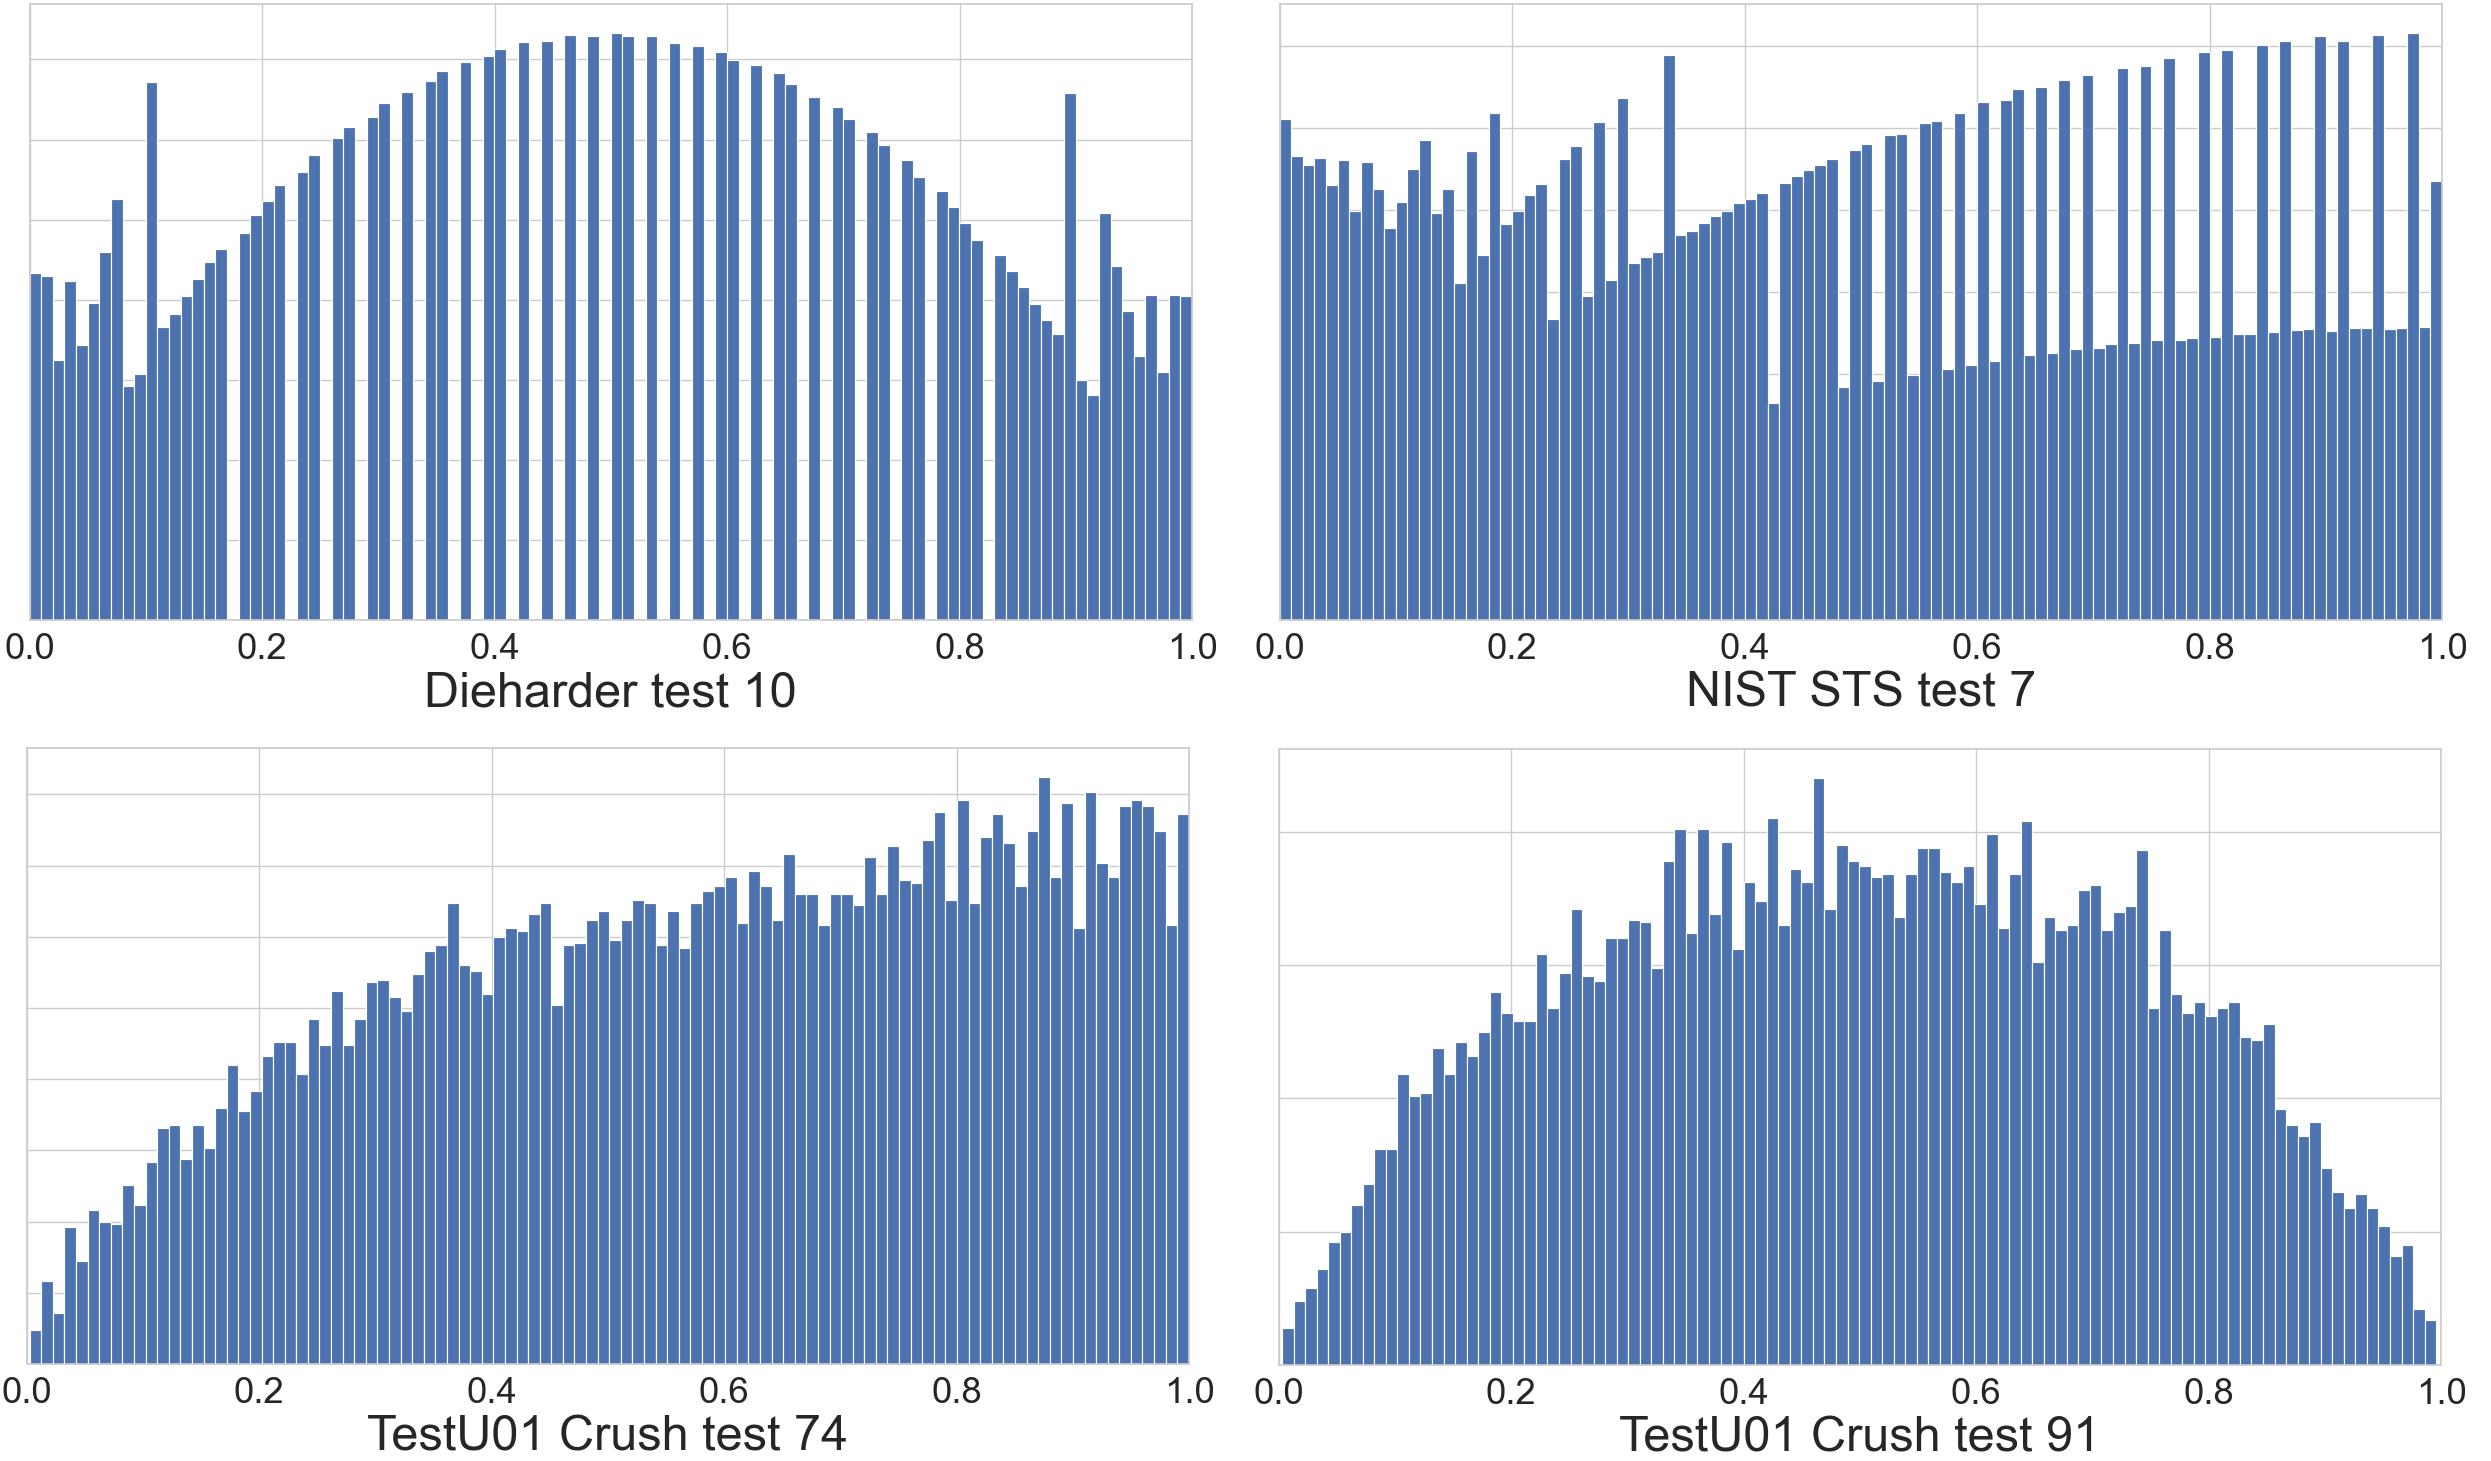
\includegraphics[width=12.5cm]{figures/uniformity.png}
  \end{center}
  \caption{Histograms for examples of non-uniform first-level p-values distributions.}
  \label{fig:uniforms}
\end{figure}

%%%%%%%%%%%%%%%%%%%%%%%%%%%%%%%
% IMPLEMENTATIONS COMPARISON
%%%%%%%%%%%%%%%%%%%%%%%%%%%%%%%

%kapitola 4.1 + 4.2:

%- na zacatku bych referencoval nejaky priklad vystupu RTT, rtt-py (klidne odkazem do prilohy).

%- "RTT reports more information..." - co presne? Tohle je strasne vagni. mozna odkaz na priklady a slovne popsat (viz predchozi bod)


\chapter{Implementations comparison} \label{chap:comparison}



The \emph{rtt-py} is supposed to be a newer version of \emph{RTT} and might replace it in the future. Therefore, in this chapter we focus mainly on finding differences between the two. The first section aims at comparing outputs of both testing toolkits. In the second section I am at finding functional differences between them, especially the features the are present in \emph{RTT} and not in \emph{rtt-py}. In the last section I present general suggestions for further improvement of both \emph{RTT} and \emph{rtt-py}. 

% COMPARE OUTPUT
% X - contents of the output
% X - parsing
%  - rtt - vše v paměti, out of memory error, dlouhé parsonvání
% X - format
% warningy - RTT parsuje slovo WARN/ERROR
% pro oba - jak parsuje výstup (paměť, ...)
\section{Output}
Example of output from \emph{RTT} can be found in Appendix \ref{append:rtt-output} and the output of \emph{rtt-py} can be found in \ref{append:rtt-py-output}. Both reports come from executions over the \emph{same} data file and using the \emph{same} battery configuration file. The output examples are shortened, but the same tests are presented in all examples if possible.

First difference in output between \emph{RTT} and \emph{rtt-py} is the format of the output. \emph{RTT} offers reports in plaintext format, which contains all of the reported information (see Subsection \ref{chap:sols-rtt}). The format is human-readable, but hard to navigate. Computer processing is possible thanks to unified format, but requires rather complicated parsing.

The \emph{rtt-py} offers an overview table in HTML and CSV formats, which are both easily human-readable and useful for quick assessment of the tests results. The CSV format is also easily computer-readable. 

The full HTML format offers more information, usually regarding the test settings. For all tests, the p-values is contained. In the NIST STS, the proportion of sequences passing the first-level test is added. In the TestU01 batteries, corresponding test statistics values are part of the HTML report as well.

The main functional difference in output between \emph{RTT} and \emph{rtt-py} are the reported information. For this comparison, the full HTML report from \emph{rtt-py} is taken. Both toolkits report the resulting second-level p-values for Dieharder and both the second-level p-value and proportion of sequences passing the first-level test for NIST STS batteries. However, unlike \emph{RTT}, the \emph{rtt-py} does not report first-level p-values, which could be useful for deeper assessment of the results. Unlike the \emph{RTT}, \emph{rtt-py} also does not report information regarding the individual tests settings (stream size and counts) from NIST STS battery.

For the TestU01 batteries (which employ only repeated single-level tests) the reported information are the same for both toolkits -- p-values and details about test settings. However, in \emph{RTT} report, repetitions of the same individual test are grouped together and their respective p-values are printed in a group. In \emph{rtt-py}, each repetition is treated as a separate individual test and the user has to manually group the tests by their names. This is important, because the TestU01 does not perform the two-level test and if the user wishes to apply it, they have to do so on their own. The FIPS and BSI batteries are not mentioned in this comparison, because they are only executed in the \emph{rtt-py}.

Both toolkits also take different approach in parsing the results. In \emph{RTT}, the results are parsed after \emph{all} tests finish their executions using regular expressions. Originally, the regular expressions used for TestU01 batteries sometimes crashed while parsing. This issue has already been fixed. \footnote{\url{https://github.com/crocs-muni/randomness-testing-toolkit/commit/7457ba6e820a886f4582f271b2b1377d14152c60}} Furthermore, when parsing large batteries outputs, the \emph{RTT} may crash due to \emph{out of memory} error.

In \emph{rtt-py}, the results are parsed after each individual test is executed and stored in pre-defined objects. After all tests from given battery are executed, corresponding report is generated.

% no errors and warns
Another part of the output of both toolkits is handling errors and warning from the batteries. The \emph{RTT} informs the user about the number of errors and warnings that occurred on the standard output. The detection of errors and warnings in \emph{RTT} is done by searching for words 'error' or 'warning' in the battery output. At the beginning of the report file, all tests that produced errors or warnings are listed. The whole line containing the warning or error is printed into the corresponding individual test report.

The \emph{rtt-py} ignores errors and warnings from test batteries. The most notable example why this is a problem are the \emph{file rewinds} (as described in Section \ref{chap:sols-batteries}).

In this case, the test will read some parts of the data more than once and inform the user about this situation. The test will still produce result, which will, however, be biased by repeated parts of the tested file. This may lead to incorrect interpretation of the results and to Type I or II error. Since the \emph{rtt-py} ignores this, there is no way for the user to be informed about this situation.
 

%%%%%%%%%%%%%%%%%%
% MISSING FEATURES
%%%%%%%%%%%%%%%%%%

% X - first-level p-values  
% X - running Crush family
% X - Test01 test-specifi
% X - detekce errors / warnings
% X - logs
% X - database connection
% rtt-py NIST folder 
% ? readiness to take new battery
% X - podívat se na paralelismus
% X - more batteries at once
\section{Implementations differences}
In this section I focus on finding the functional differences between \emph{RTT} and \emph{rtt-py}. The primary goal is to find features, that are missing in the \emph{rtt-py} and should be implemented to allow the replacement of \emph{RTT} with \emph{rtt-py}. 




% used batteries difference
Both \emph{RTT} and \emph{rtt-py} employ different set of batteries. The Dieharder, NIST STS, TestU01 Rabbit, Alphabit and BlockAlphabit batteries are run in both implementations. The FIPS and BSI batteries are only executed in the \emph{rtt-py}. The TestU01 \emph{Crush} family of batteries is only run by \emph{RTT}. The program options of \emph{rtt-py} however clearly suggest, that these batteries should also be run. There is no explanation why neither in \cite{vavercak} or \cite{rtt-py-site}.

% Running more batteries at once
Regarding the batteries, the \emph{RTT} runs one user-chosen battery per run. In the \emph{rtt-py}, all batteries are run by default. The user can choose batteries to omit from the run. The \emph{RTT} runs either all tests from the current battery configuration, or only single test chosen by the user, while in \emph{rtt-py} all tests from given configuration are run. Also the \emph{rtt-py} allows the user to test more files with data during one run, while \emph{RTT} allows testing of a single file only.

% test specific settings - requires dieharder and nist, tu01 ignores repetitions
Another difference between toolkits is handling the \emph{test-specific-settings} field from battery configuration files. In \emph{RTT}, this field is optional for all batteries. However, in \emph{rtt-py} this field is \emph{required} for Dieharder and NIST STS battery and the configuration will not parse otherwise. This may cause problems with compatibility of configuration files between \emph{RTT} and \emph{rtt-py}.

Another difference with this field is that \emph{rtt-py} ignores \emph{repetitions} field from \emph{test-specific-settings} of TestU01 batteries, therefore all test are executed with. This also might to be the reason why \emph{Crush} family batteries are not run, because this field is needed for \emph{meaningful} use of the \emph{Crush} family batteries, while the remaining TestU01 batteries can be \emph{meaningfully} used without changing the \emph{repetitions} argument.



% no logs
Closely tied with the warnings and errors are the output logs of the executed batteries. They are usually used to examine the warnings and errors raised by the batteries and to decide about the severity of the warning or error. Another usage may be to examine further details of the report that are not reported by the used toolkit. 

In \emph{RTT}, the output logs for each battery are stored in the \emph{results} folder. In \emph{rtt-py}, no batteries output logs are being stored. Both \emph{RTT} and \emph{rtt-py} create run logs containing the exact arguments used to run the batteries.

% pvals printout + error
As was described in previous section, unlike \emph{RTT}, the \emph{rtt-py} does not report first-level p-values from Dieharder and NIST STS. The first-level p-values can be usefull for deeper examination of the tests results. In TestU01, the p-values are grouped by test in \emph{RTT}, but not in \emph{rtt-py}. Furthermore, as opposed to \emph{RTT}, the \emph{rtt-py} ignores the warning from battery outputs.


% paralelism
The \emph{RTT} allows parallel execution of several individual tests at once (maximal number of parallel exectuions is set by the user in \emph{rtt-settings.json} file). In \emph{rtt-py}, no parallelism is supported and all individual tests are executed serially. 

% adding new battery
One of the original ideas of \emph{RTT} was to provide interface for easy addition of new batteries, possibly by the user. In \emph{rtt-py}, the user only has to implement classes for settings parsing, executions and results parsing, which all follow predefined patterns. These classes are then easily integrated into the \emph{rtt-py}.

Compared to this, the source code of \emph{RTT} is much more interconnected. The user has to implement several classes regarding the executions and results parsing as well. For the settings parsing, however, the user has to extend the already existing class. The user also has to extend several another classes responsible for setting up and executing the batteries. That makes adding a new battery into the \emph{RTT} harder than into the \emph{rtt-py}

% database
The \emph{RTT} also offers storing the test results in configured database, which is not offered by the \emph{rtt-py}. This functionality is, however, often not used. Because the used database connection is not supported on some Unix distributions, the \emph{RTT} may be compiled without it.

\begin{table}[t]
  \begin{tabularx}{\textwidth}{l|l|l}
    Feature & RTT & rtt-py \\
    \midrule
    \midrule
    Missing batteries & FIPS, BSI & TestU01 SmallCrush, \\ %
     & & Crush, BigCrush \\
    \midrule
    %nist folder & manually & added argument \\
    %\midrule
    Dieharder and NIST & yes & no \\ %
     first-level p-values & & \\
    \midrule
    TestU01 p-values from  & grouped & each repetition \\
     single individual test  & &  separate \\
    \midrule
    Battery errors and warning & yes & no \\ %
    \midrule
    Battery output logs & yes & no \\ %
    \midrule
    Run logs & yes & yes \\
    \midrule
    Parallel executions & yes & no \\ %
    \midrule
    Readiness for new battery & less & more \\
    \midrule
    Batteries in one run & single & all \\
    \midrule
    Tests in one run & all or single & all \\
  \end{tabularx}
  \caption{Overview table comparing the features of \emph{RTT} and \emph{rtt-py}.}
  \label{tab:comparison}
\end{table}


% rtt-py adding first-level p-values
% rtt-py adding errors
% X - tests setup - config calc
% X - our own second-level assessment
% X - computer - readable format
% RTT-Tu01 - co dělá
% pro tu01 - přidat detekc rewindu
\section{Proposed improvements}
First proposed improvement for both \emph{RTT} and \emph{rtt-py} is better way to configure the batteries. While \emph{RTT} offers some prepared configuration files, they are not available for all file sizes. Also, some of the configuration files contained configurations that resulted in \emph{file rewinds} or the tests read less data than was possible, resulting in testing only a part of the file. I implemented this improvement in the form of Configuration Calculator (see Subsection \ref{chap:analysis-config-calc}).

Second proposed improvement are better second level-tests. As is shown in Subsection \ref{chap:analysis-uniform}, p-values of many first-level tests do not follow the uniform distribution. The improved second-level tests should take these non-uniform distributions into account and compare the observed distributions to the real distributions of the tests. The improved second-level tests also should provide second-level assessment of the TestU01 batteries.

Third proposed improvement is to extend the output format of \emph{RTT} to computer-readable format, possibly using JSON format as in configurations. This could be used not only for quick computer-made results assessments, but also for the custom second-level tests.


%%%%%%%%%%%
% CONCLUSION
%%%%%%%%%%%%%%
\chapter{Conclusion}

% intro
%Primary goal of this thesis was to analyse \emph{Randomness Testing Toolkit} and its newer, alternative implementation, the \emph{Randomness Testing Toolkit in Python}. First part of the analysis focused on finding differences between the two, which prevent replacement of \emph{RTT} with \emph{rtt-py}. The second part of the analysis proposed improvements, that might improve performance and usability of both \emph{RTT} and \emph{rtt-py}.

% intro theory + solutions
%This thesis explained the two main approaches to randomness testing (one-level and two-level tests) so that the readers can fully understand it. The explanation is followed by description of notable programs for randomness testing.

% intro analysis
We analysed the \emph{Randomness Testing Toolkit} and its newer, alternative implementation, the \emph{Randomness Testing Toolkit in Python}. The analysis focused on finding differences between the two implementations in order to allow future replacement of \emph{RTT} with \emph{rtt-py}, and on proposing improvements for both toolkits.

% test analysis 
First, we analysed the individual tests present in the randomness testing batteries. During the tests analysis we collected information about \emph{data consumption} and \emph{runtimes} of the individual tests. We used the data to detect tests with low performance. As such were marked TestU01 Crush tests with ID 71 and 72, and TestU01 Rabbit test with ID 5. In the future, the data may be used for further analysis in combination with other factors (for example "strength" of the test).

% config calc
We created the \emph{Configuration Calculator} based on the data from the tests analysis -- tool for automated creation of battery configuration files for both \emph{RTT} and \emph{rtt-py}. This tool has already been used by CRoCs and will be published to use with the \emph{RTT}.

% implementations comparison
We performed the analysis of both \emph{RTT} and \emph{rtt-py} by comparing the features of both implementations. The focus was on output of the toolkits (both format of the reports and the information contained in them) and features, that are missing in the \emph{rtt-py} compared to the \emph{RTT}.

%From the implementations analysis arose list of features missing in \emph{rtt-py}, that prevent it from replacing the \emph{RTT}, and a list of proposed improvements for both implementations.
 The most notable differences between \emph{RTT} and \emph{rtt-py} are the output format (plaintext in \emph{RTT}, HTML in \emph{rtt-py}) and that, unlike \emph{RTT}, the \emph{rtt-py} does not report first-level p-values for Dieharder and NIST STS battery. Furthermore, the \emph{rtt-py} does not report errors from batteries. In regard to functionality, \emph{rtt-py} does not contain TestU01 \emph{Crush} family of batteries and \emph{RTT} does not contain FIPS and BSI batteries. The proposed improvements for both toolkits are to implement second-level tests which take into account the non-uniform distributions of first-level p-values of the individual tests, and computer-readable format of the ouput. 

% future work
In the future, this thesis can be followed by implementing the missing features of the \emph{rtt-py} listed in the implementations comparison, so that it can fully replace the older \emph{RTT}. Furthermore, both \emph{RTT} and \emph{rtt-py} can be extended based on the proposed improvements from the last chapter, particularly the improved second-level tests. 


%%%%%%%%%%%%%%%%%%
%% APPENDICES
%%%%%%%%%%%%%%%%%%
\appendix 

\chapter{Batteries output examples} \label{append:dieharder-output}
\section{Dieharder}

\begin{figure}[h]
  \begin{center}
    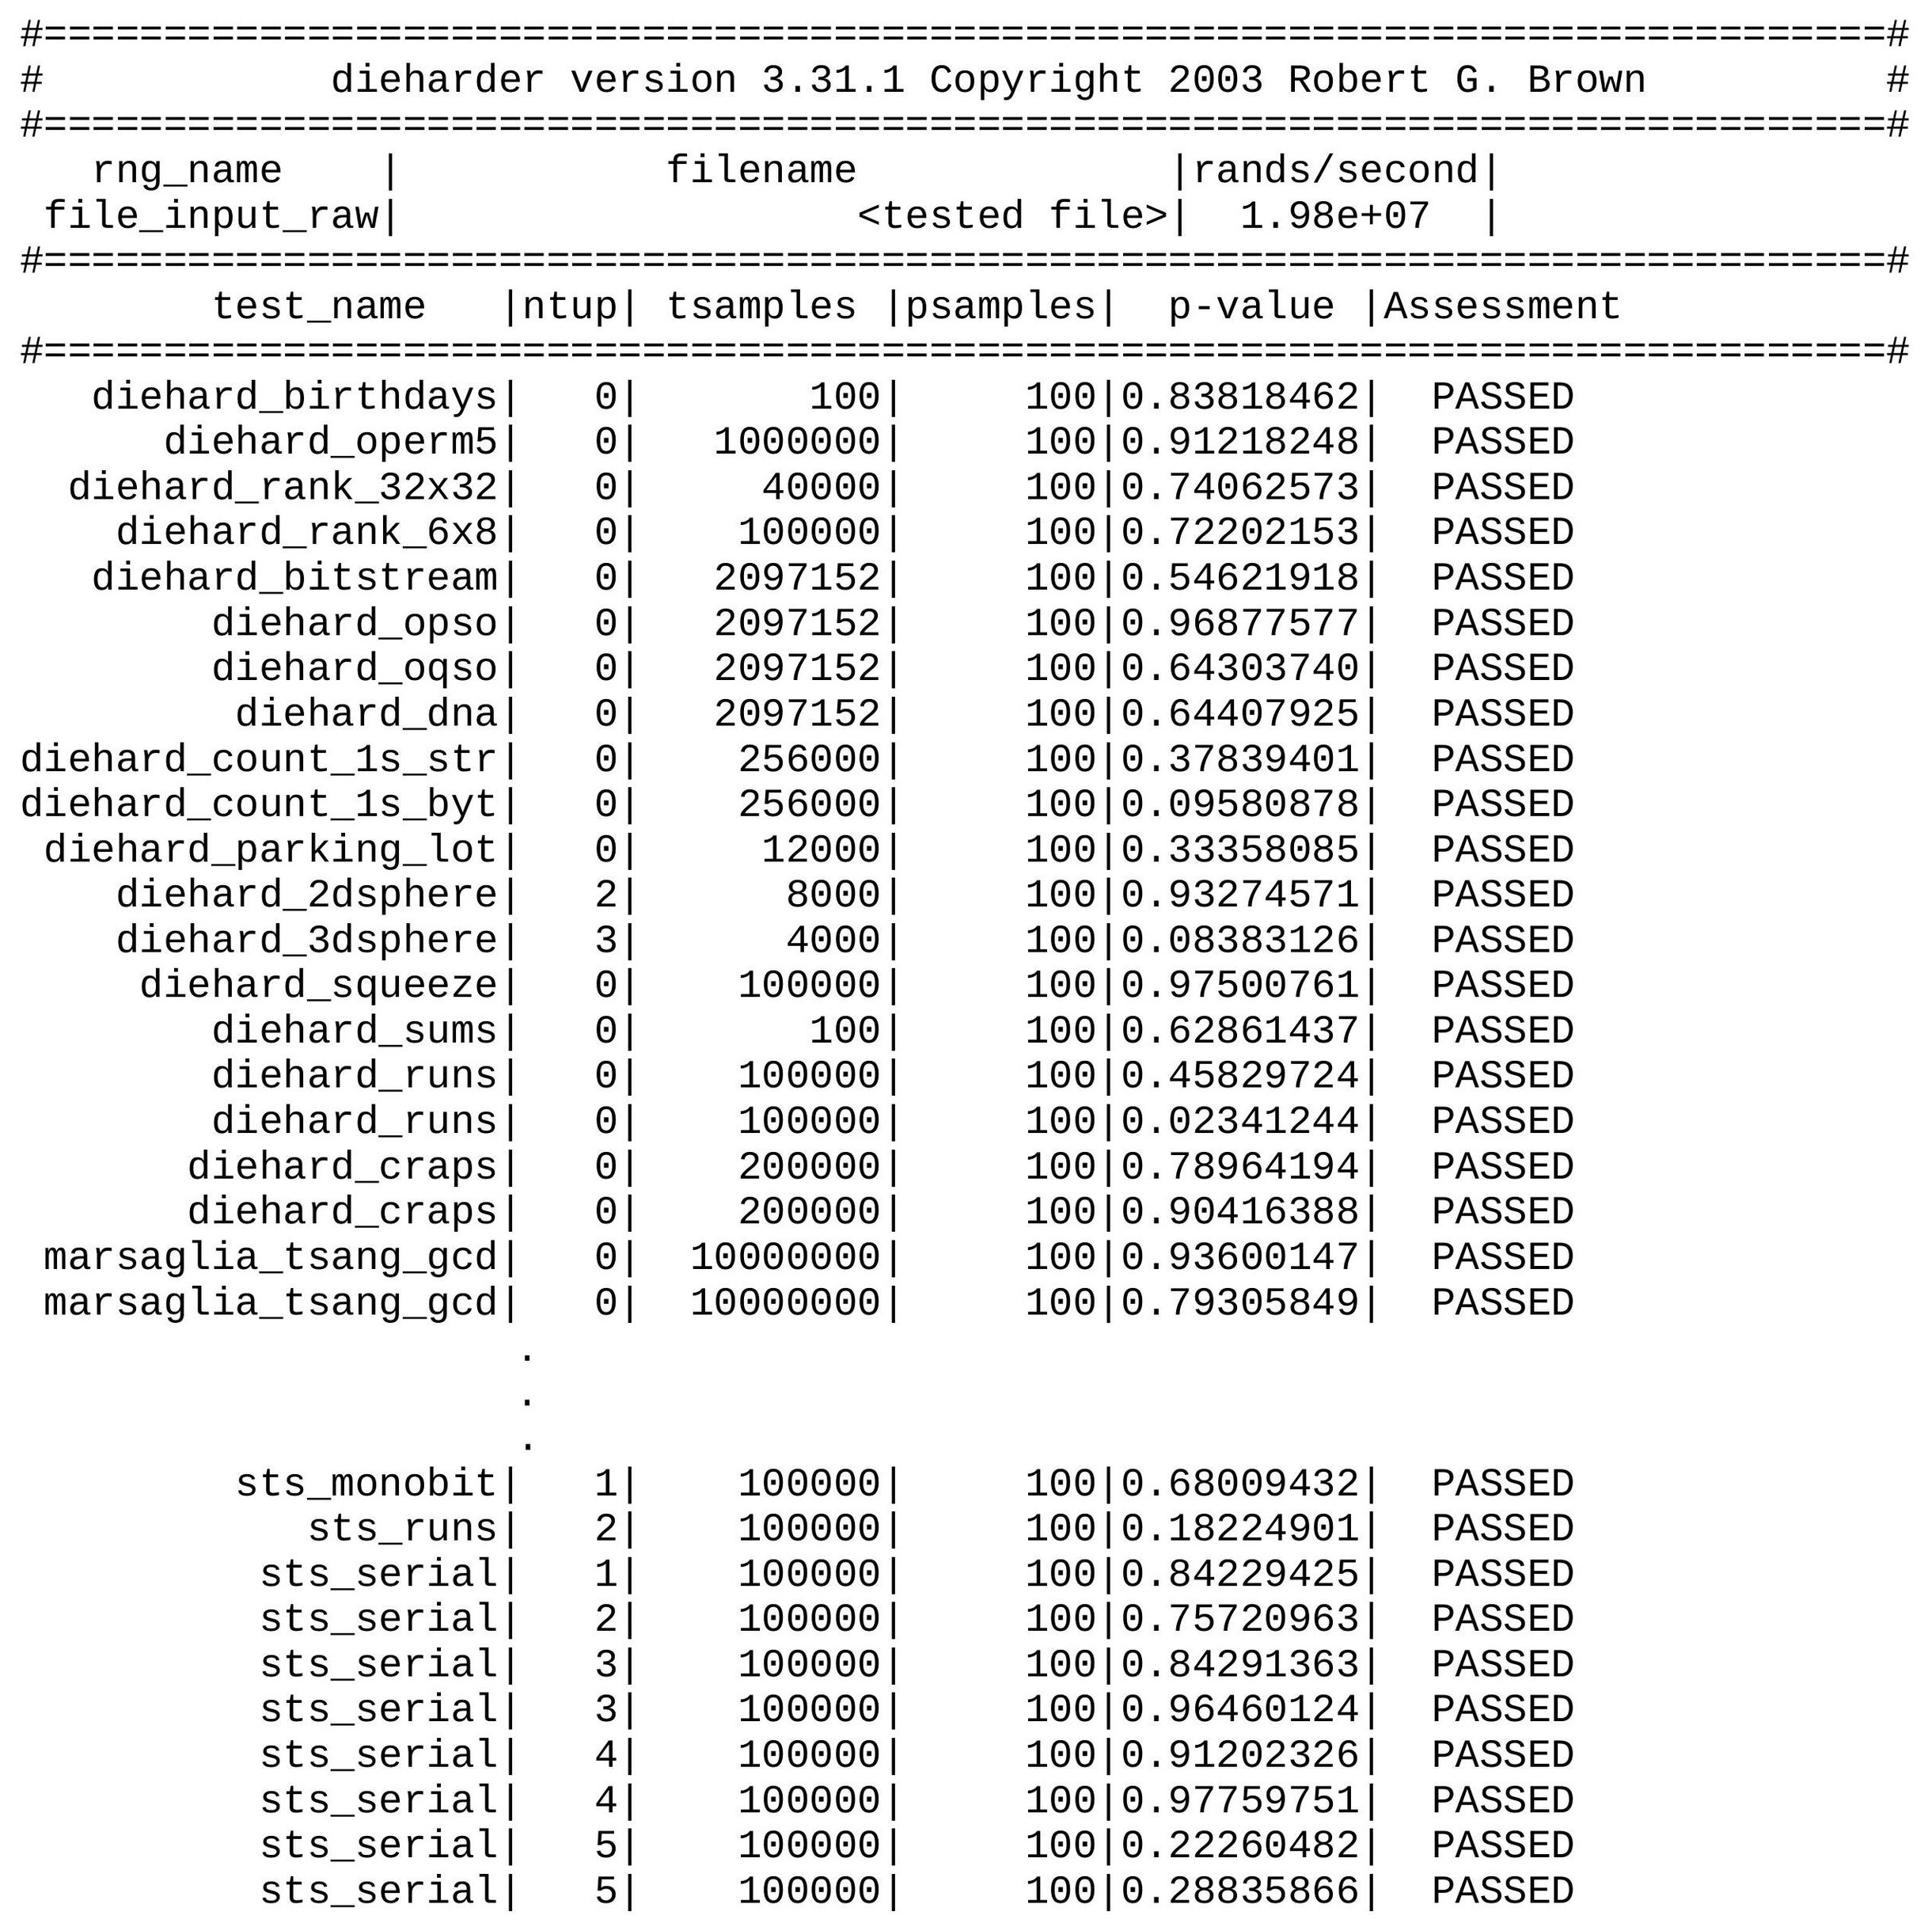
\includegraphics[width=12.5cm]{figures/outputs-appendix/dieharder.jpg}
  \end{center}
  \caption{Example of results table from the \emph{Dieharder} battery.}
  \label{fig:die_out}
\end{figure}

\newpage

\begin{figure}[h]
  \begin{center}
    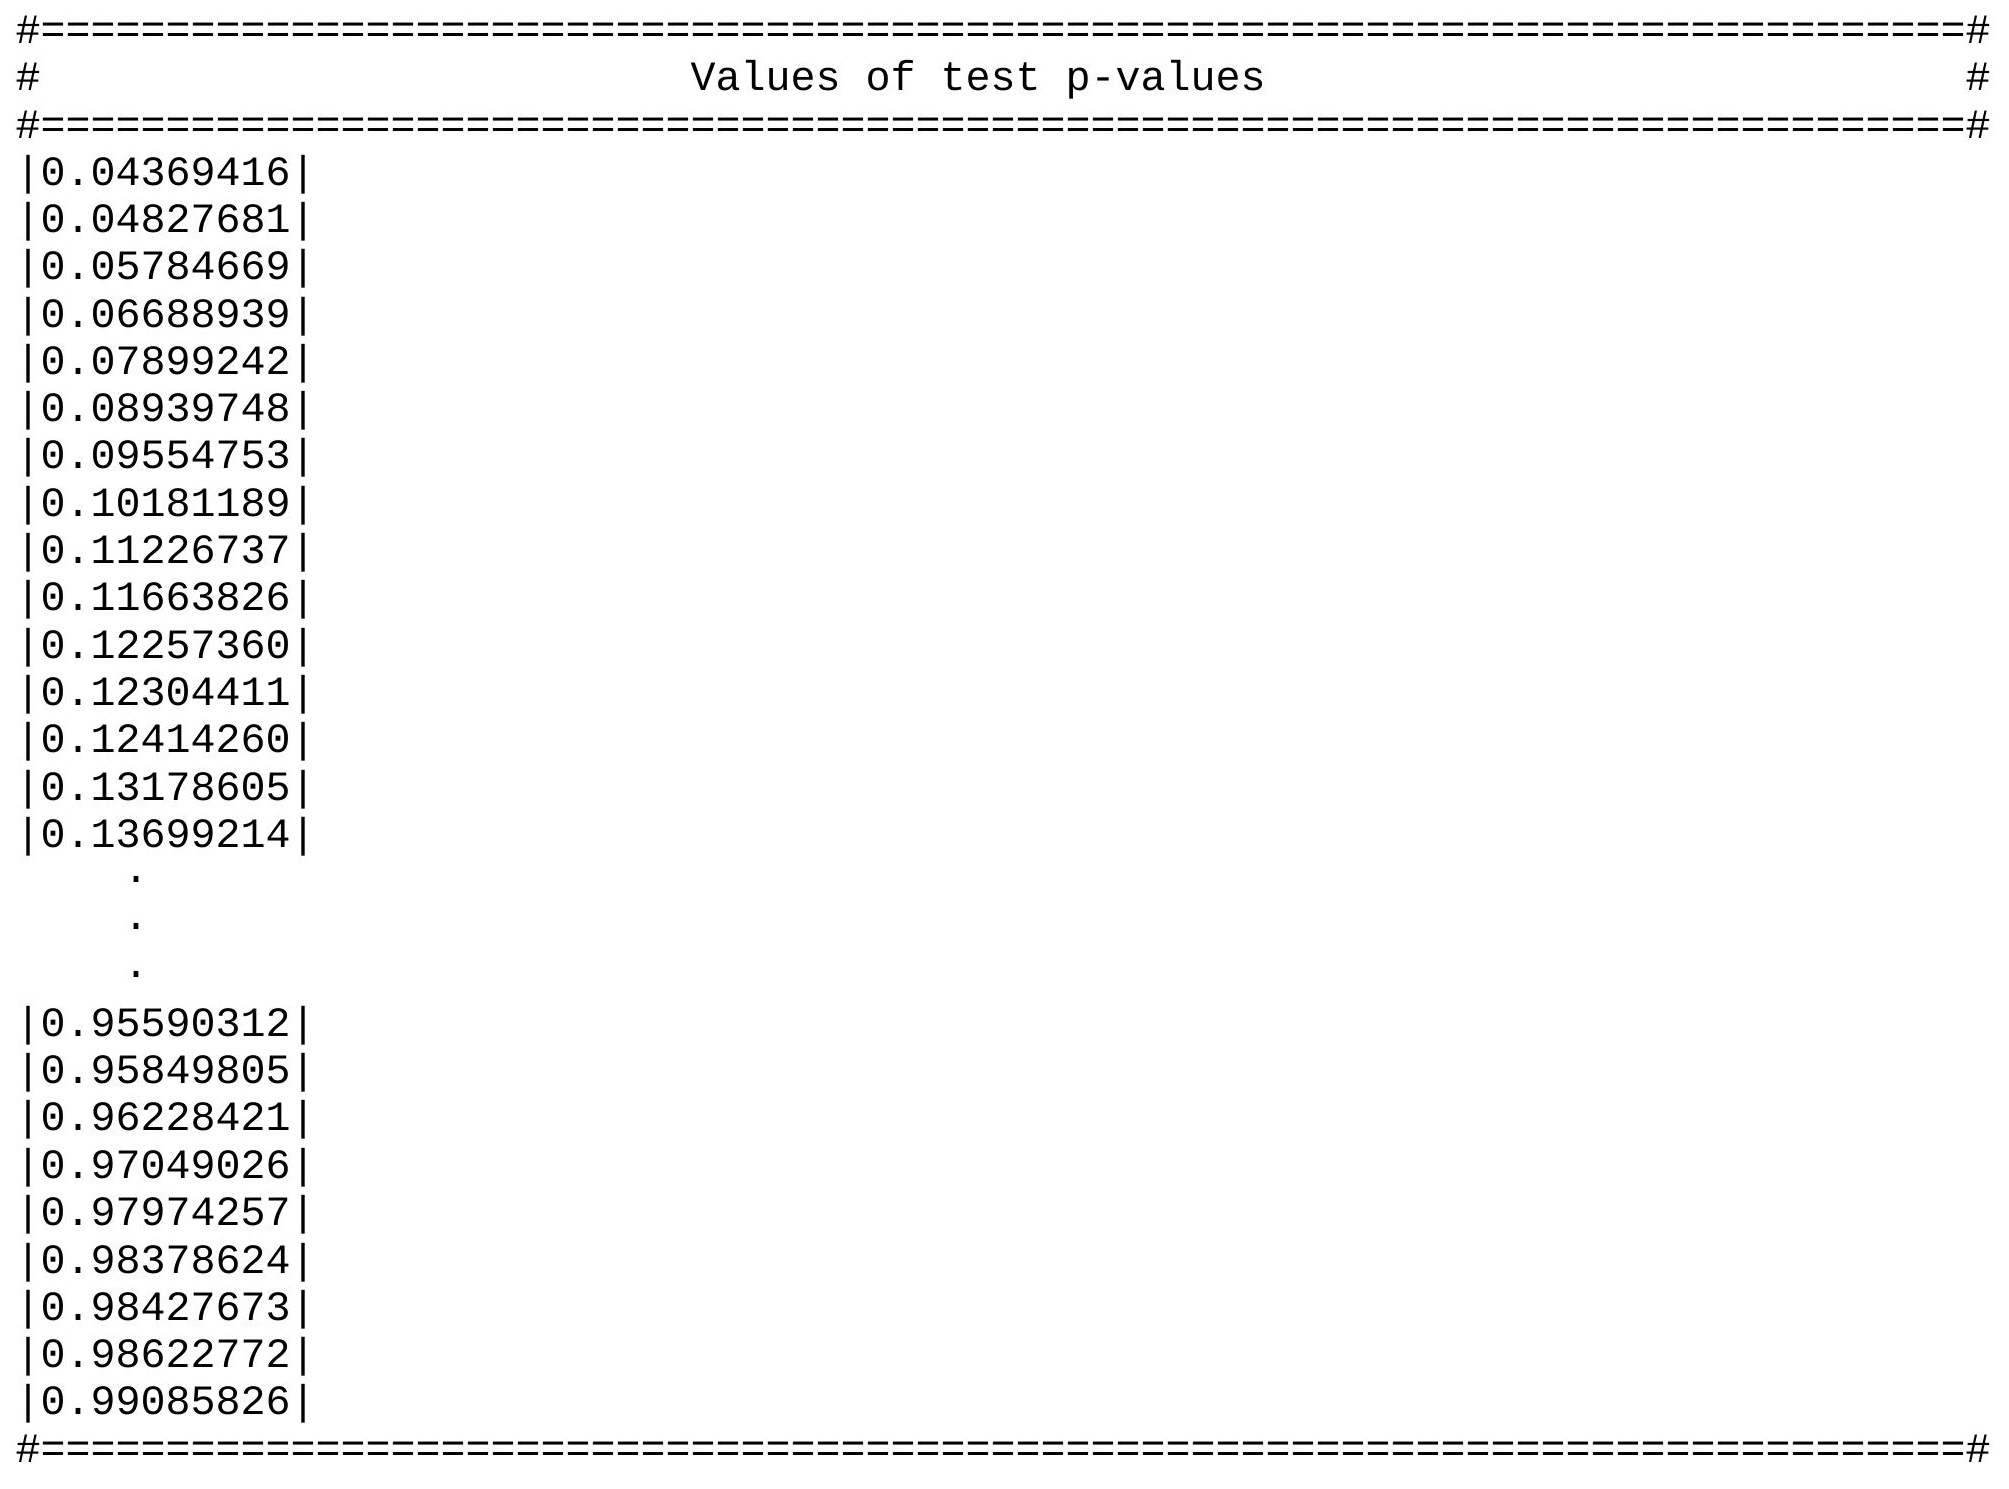
\includegraphics[width=12.5cm]{figures/outputs-appendix/pvals.jpg}
  \end{center}
  \caption{Example of first-level p-values printout from \emph{Dieharder} battery}
  \label{fig:die_pvals}
\end{figure}

\newpage

\section{NIST STS} \label{append:nist-output}

\begin{figure}[h]
  \begin{center}
    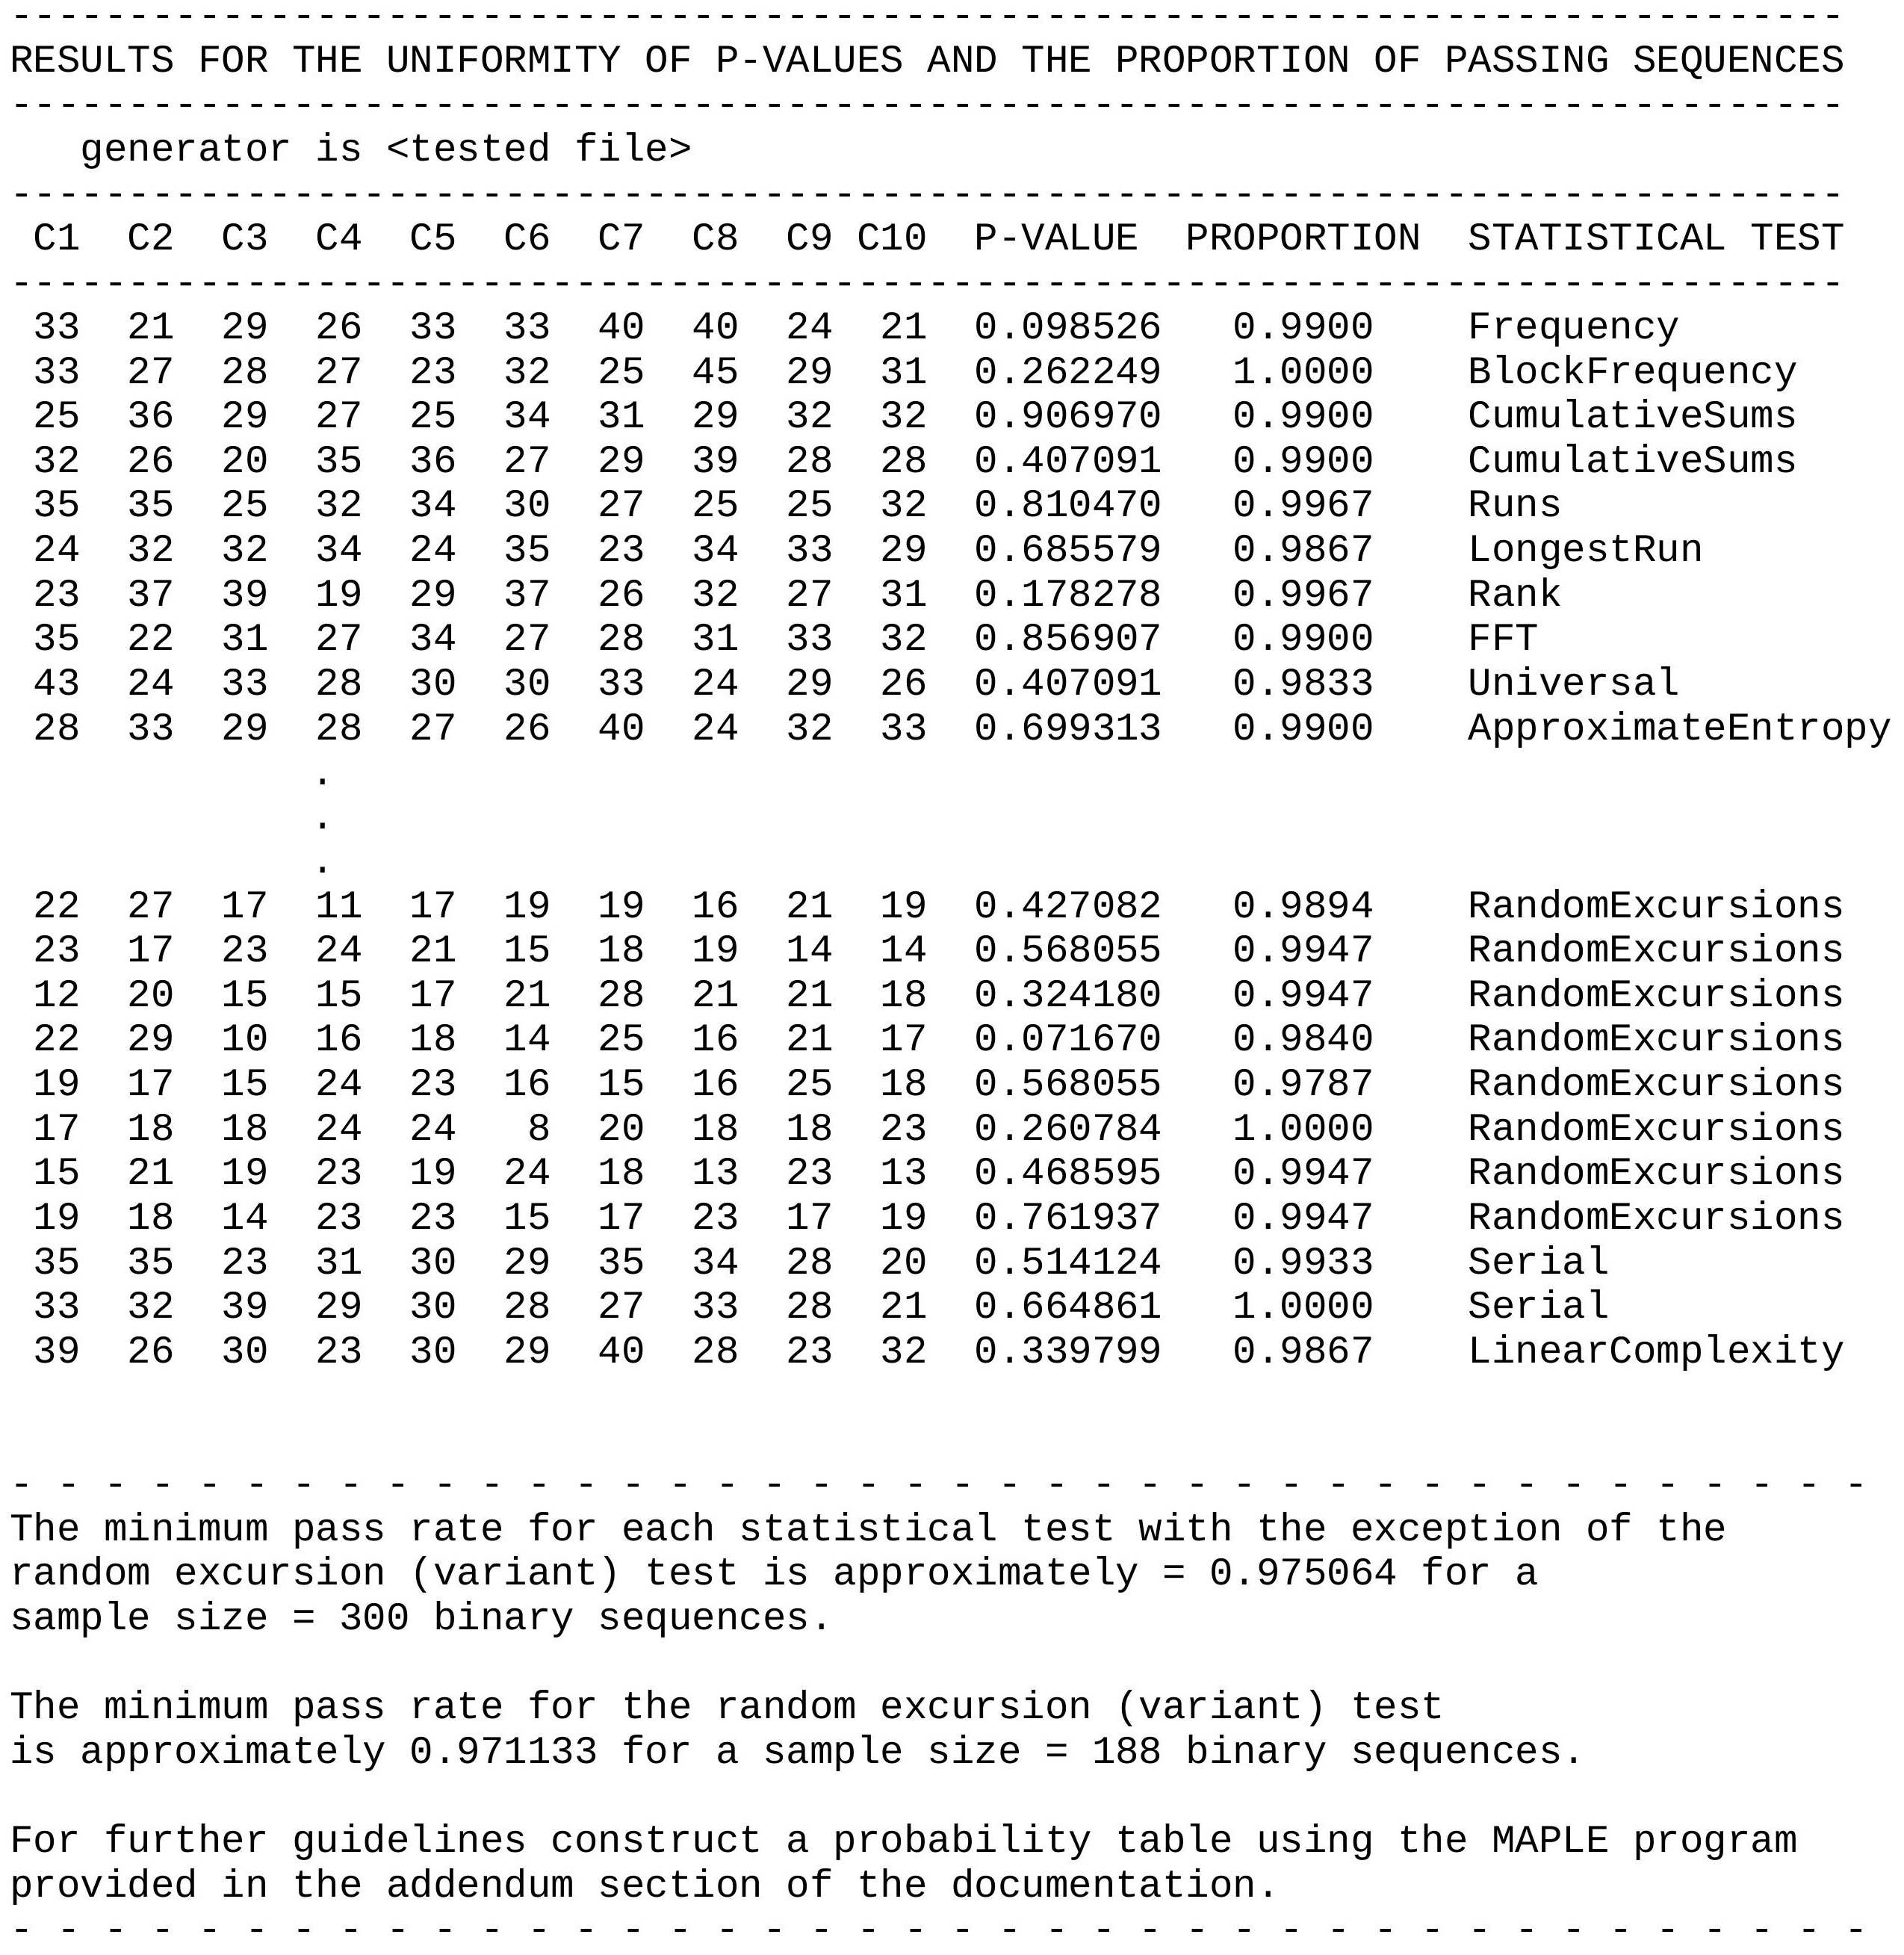
\includegraphics[width=12.5cm]{figures/outputs-appendix/finalAnalysisReport.jpg}
  \end{center}
  \caption{Example of results table from the \emph{NIST STS} battery.}
  \label{fig:nist_tab}
\end{figure}

\newpage

\begin{figure}[h]
  \begin{center}
    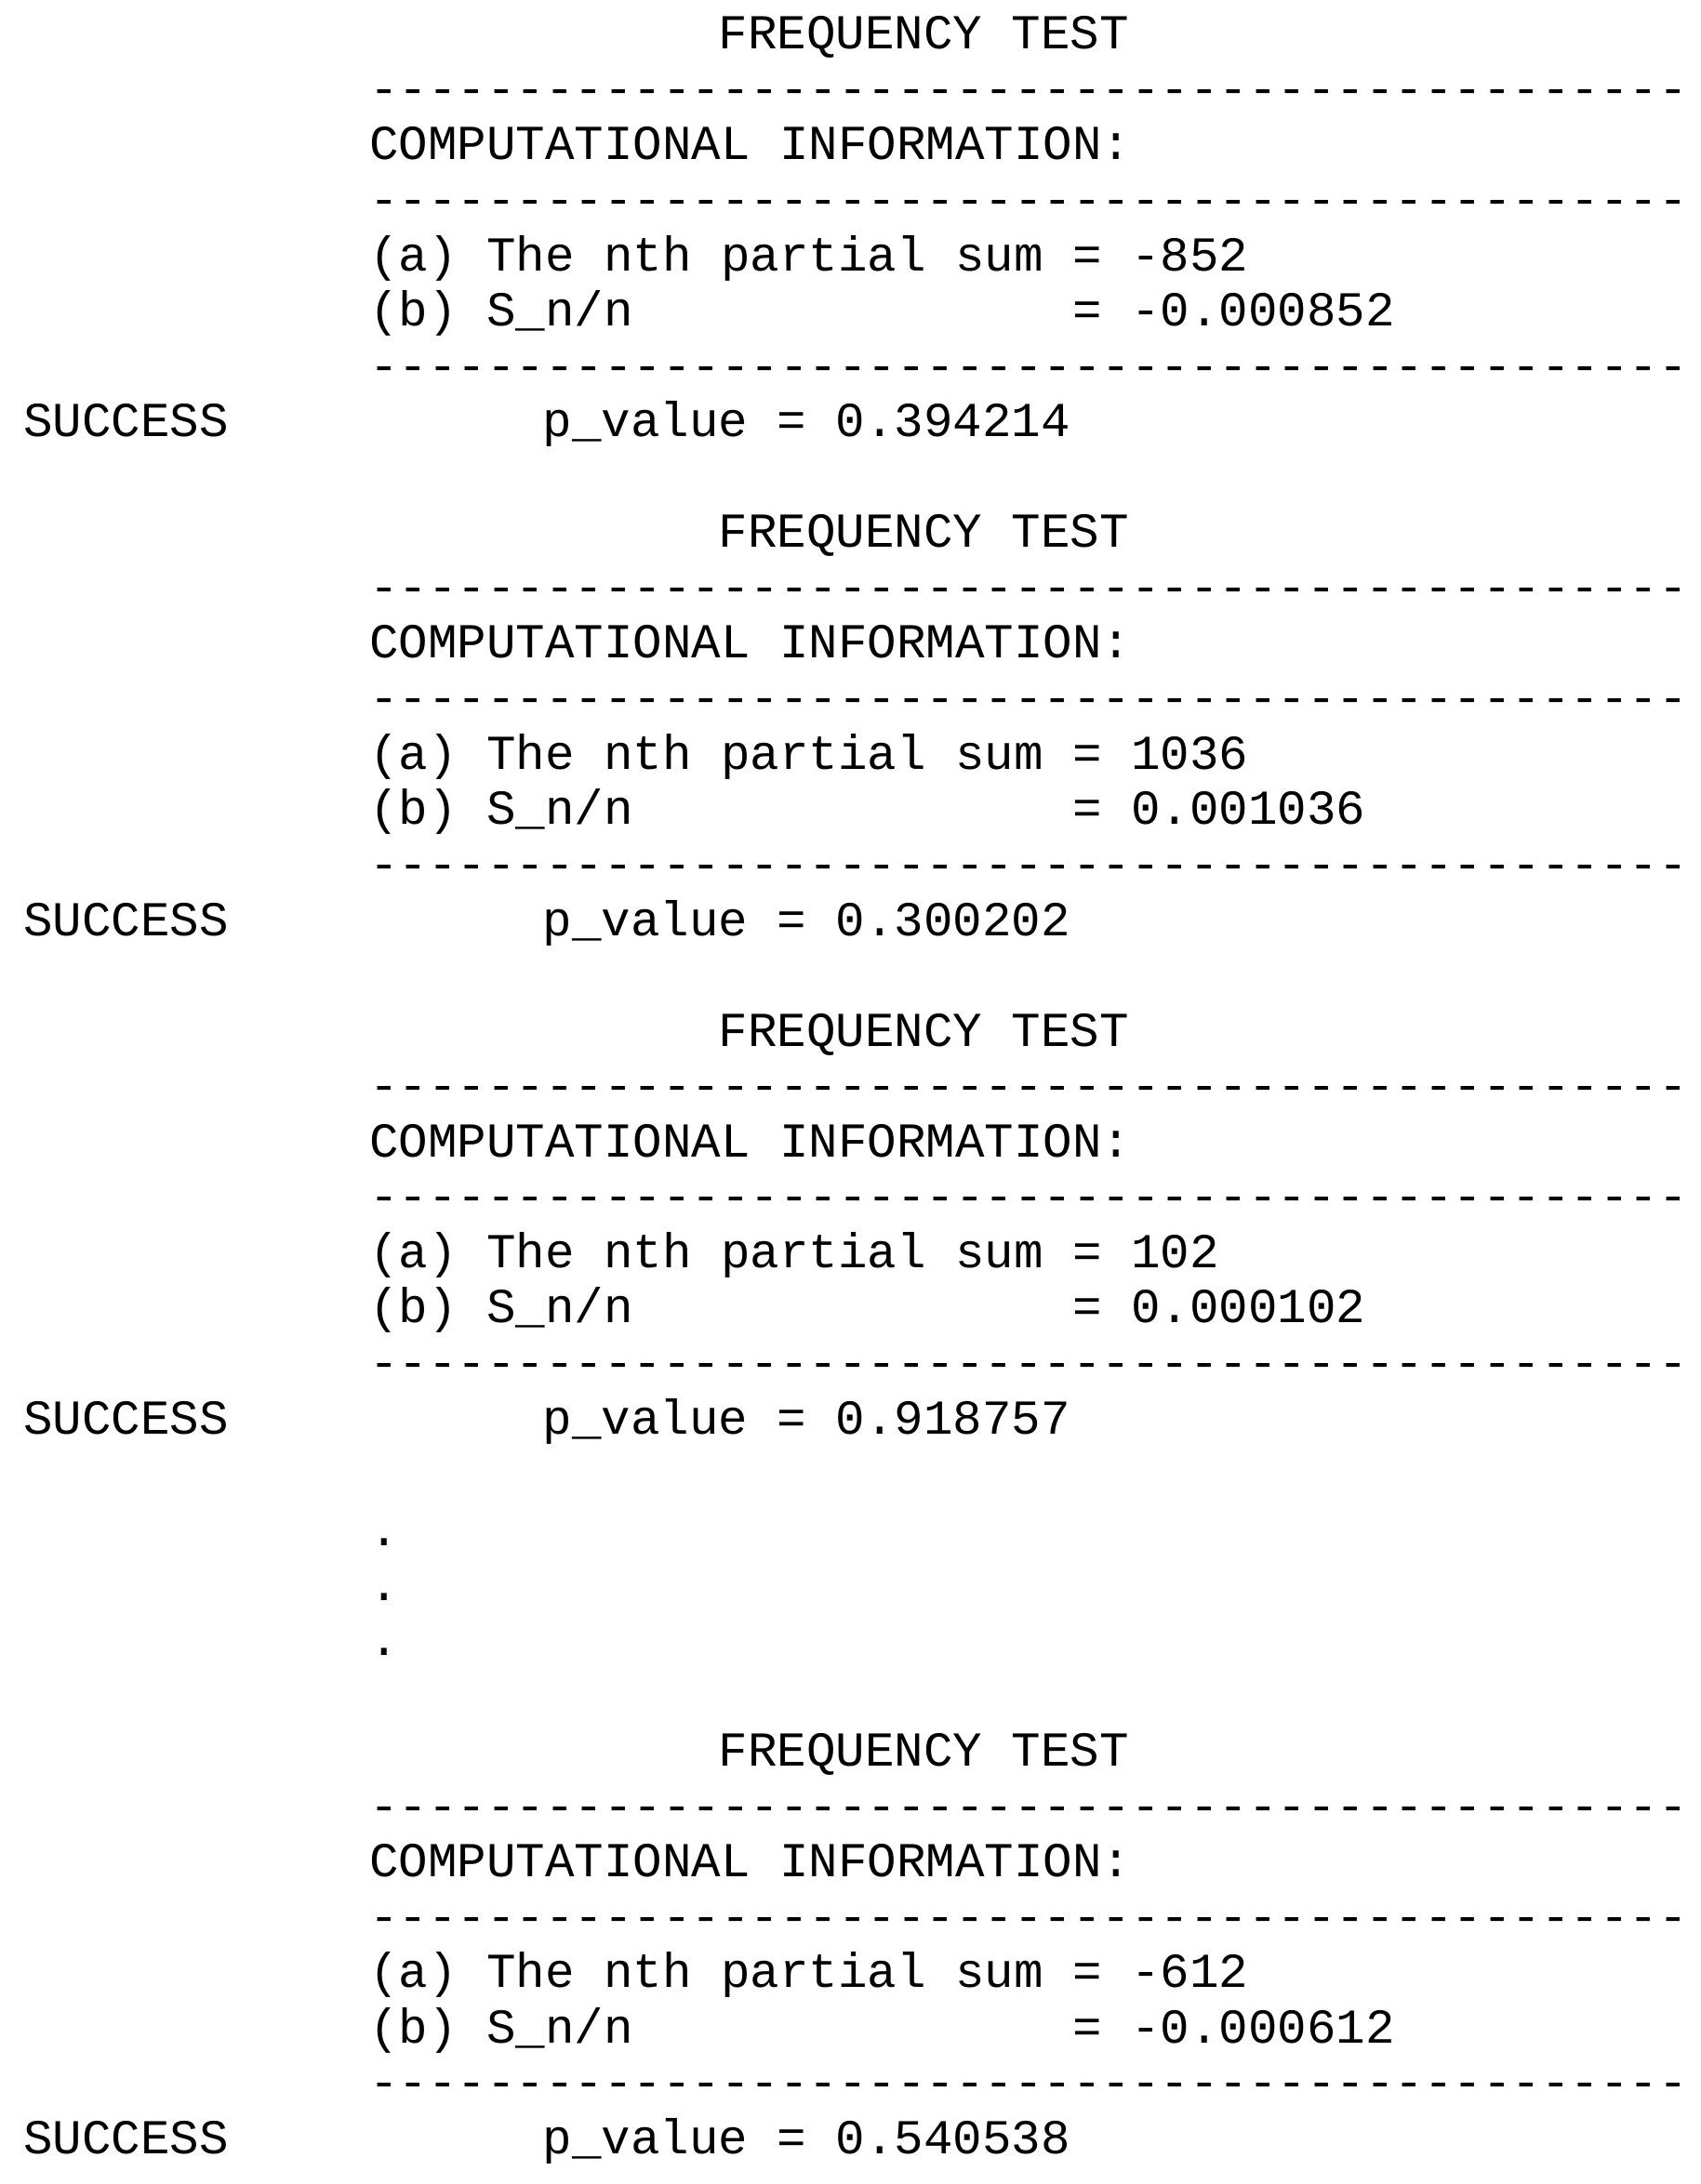
\includegraphics[width=9cm]{figures/outputs-appendix/stats.jpg}
  \end{center}
  \caption{Example of p-values, test statistics and other information from NIST STS's \emph{stats.txt} file.}
  \label{fig:nist_stats}
\end{figure}

\newpage

\section{TestU01} \label{append:tu01-output}

\begin{figure}[h]
  \begin{center}
    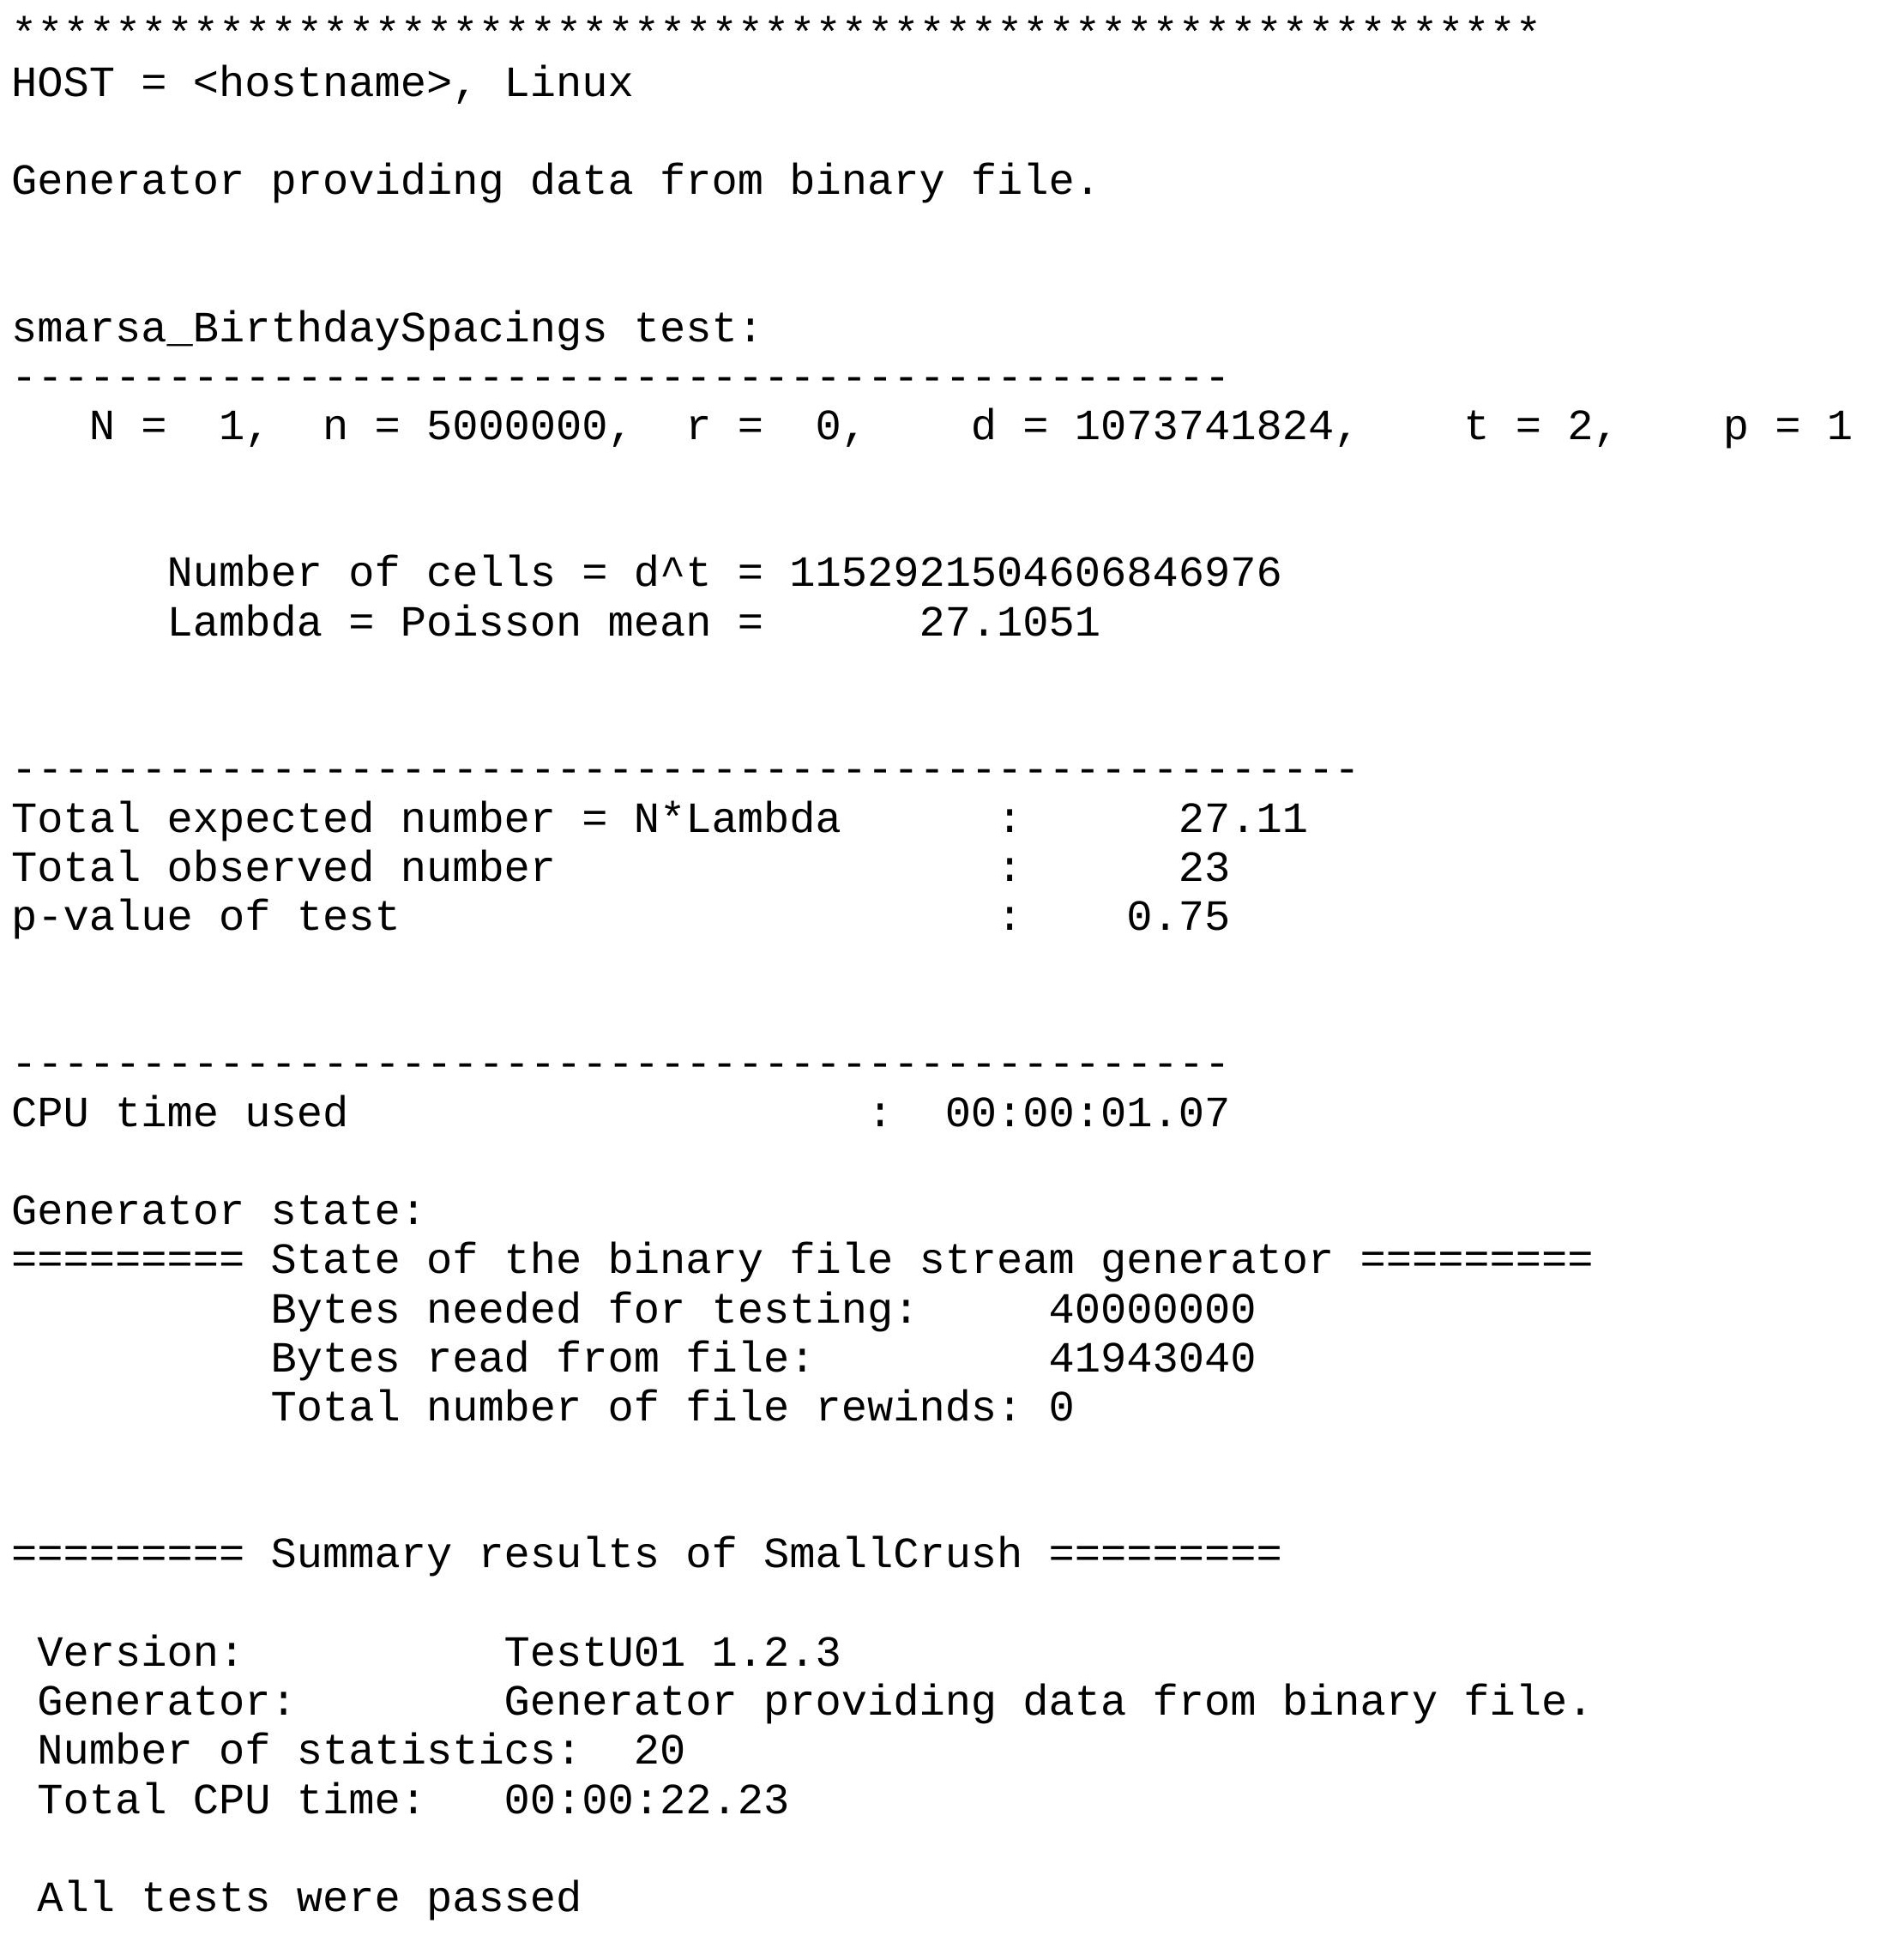
\includegraphics[width=12.5cm]{figures/outputs-appendix/tu01single.jpg}
  \end{center}
  \caption{Example of individual test repetition
   report from \emph{TestU01} SmallCrush battery. }
  \label{fig:tu01single}
\end{figure}

\newpage

\begin{figure}[h]
  \begin{center}
    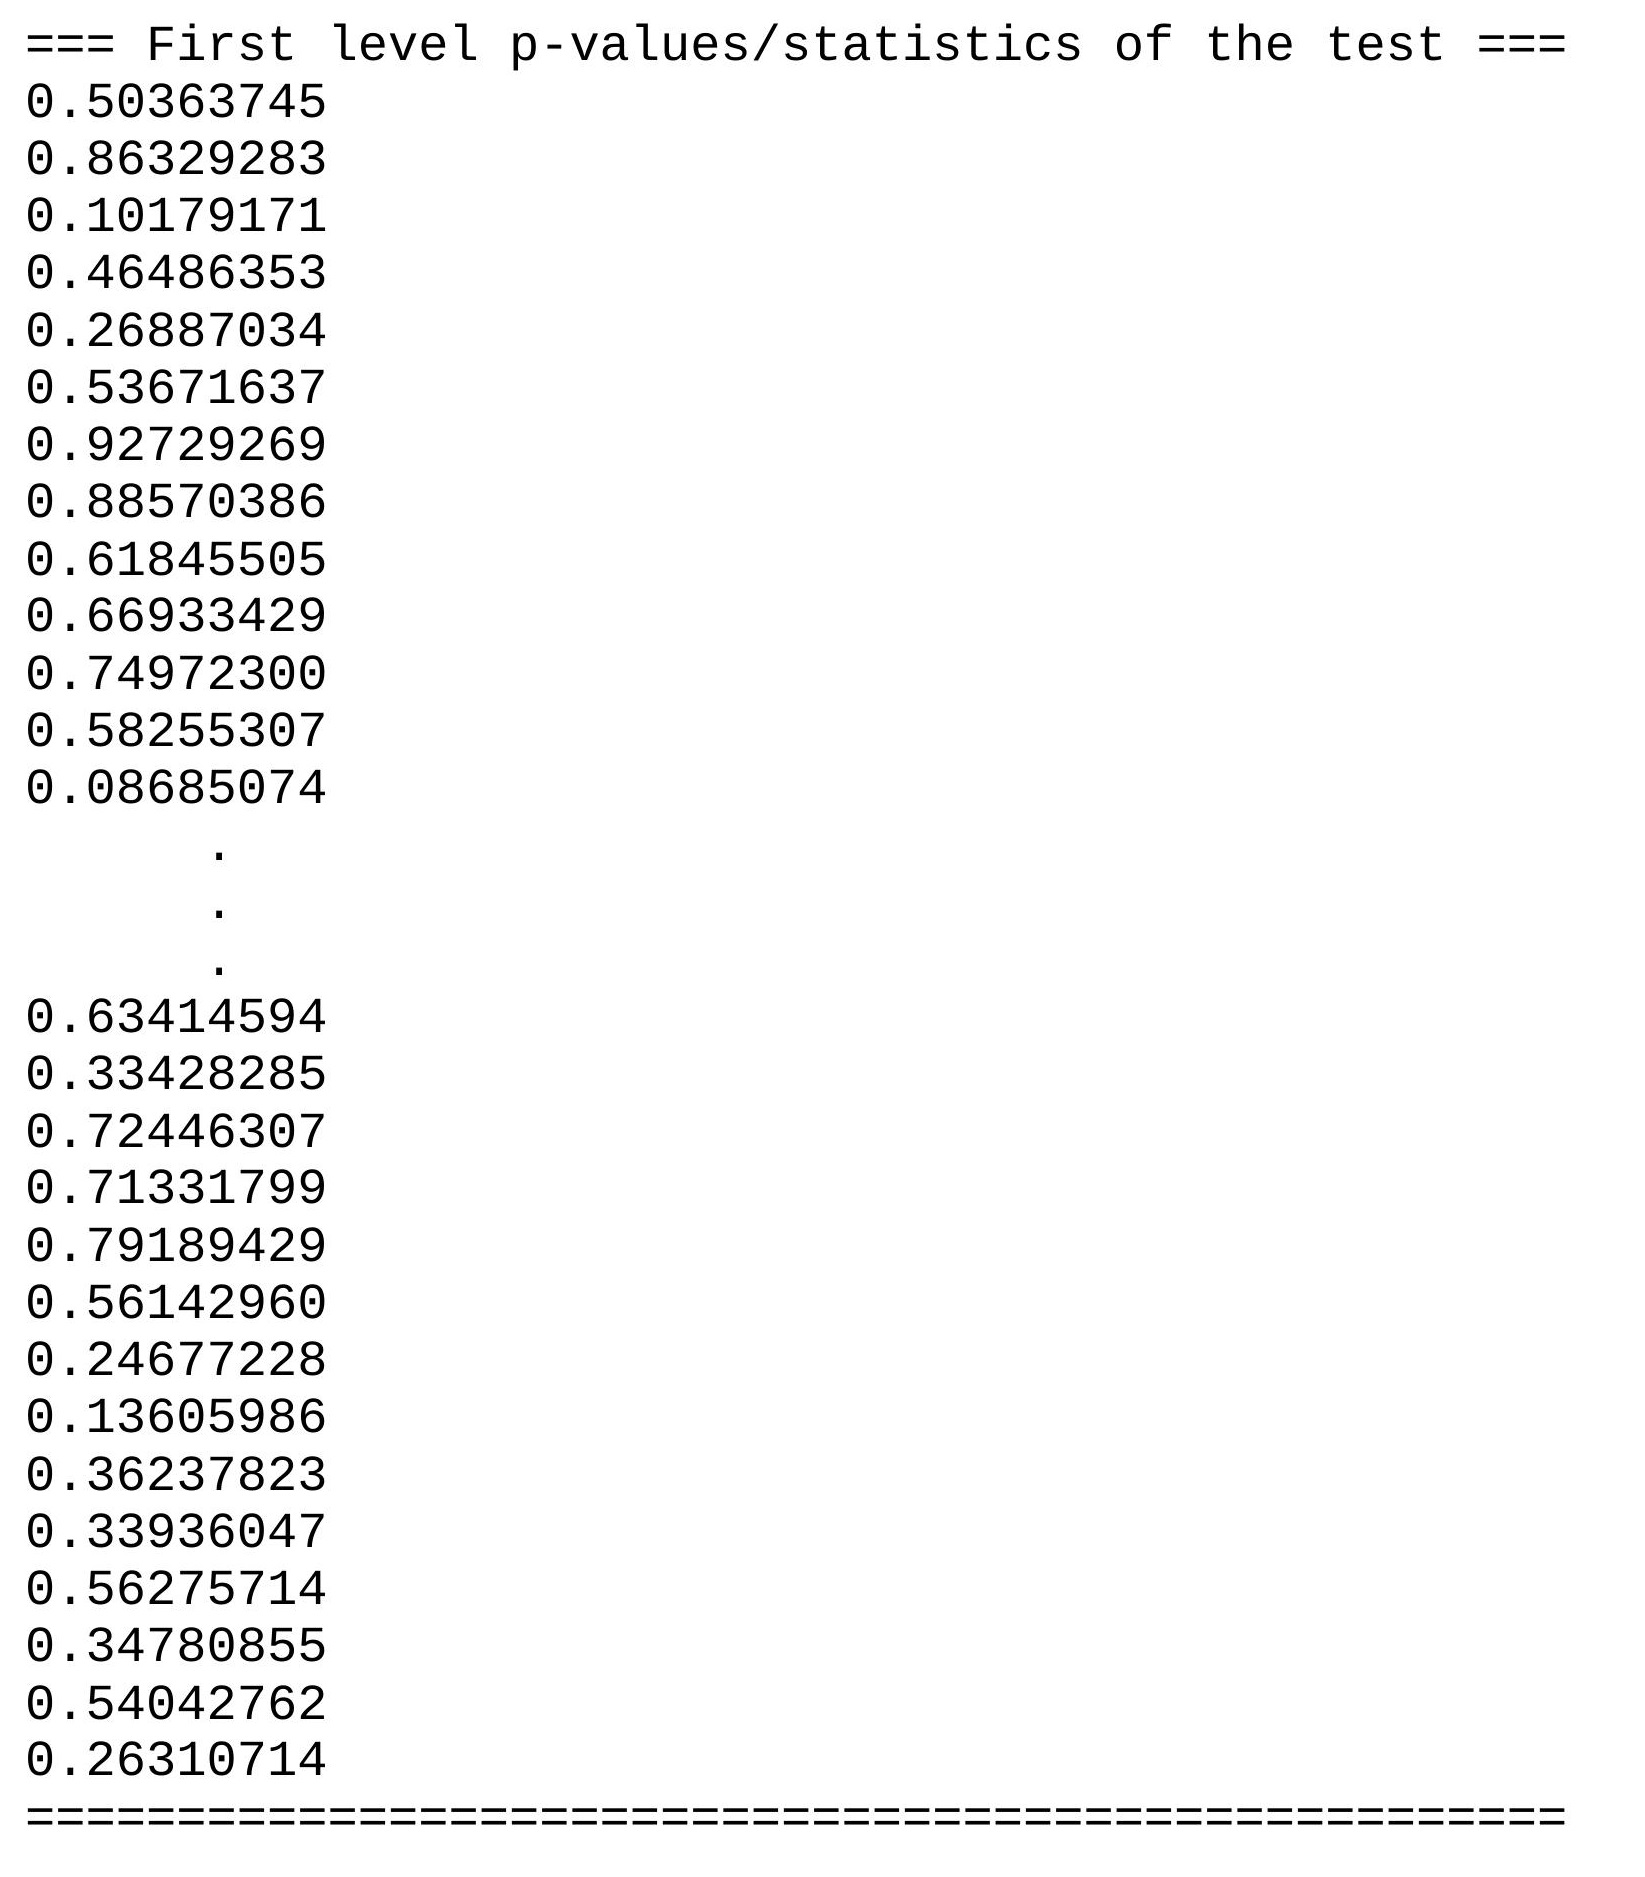
\includegraphics[width=10cm]{figures/outputs-appendix/testu01pvalues.jpg}
  \end{center}
  \caption{Example of p-values printout from \emph{TestU01} battery.}
  \label{fig:tu01pvalues}
\end{figure}

\newpage

\section{FIPS battery} \label{append:fips-output}
\begin{figure}[h]
  \begin{center}
    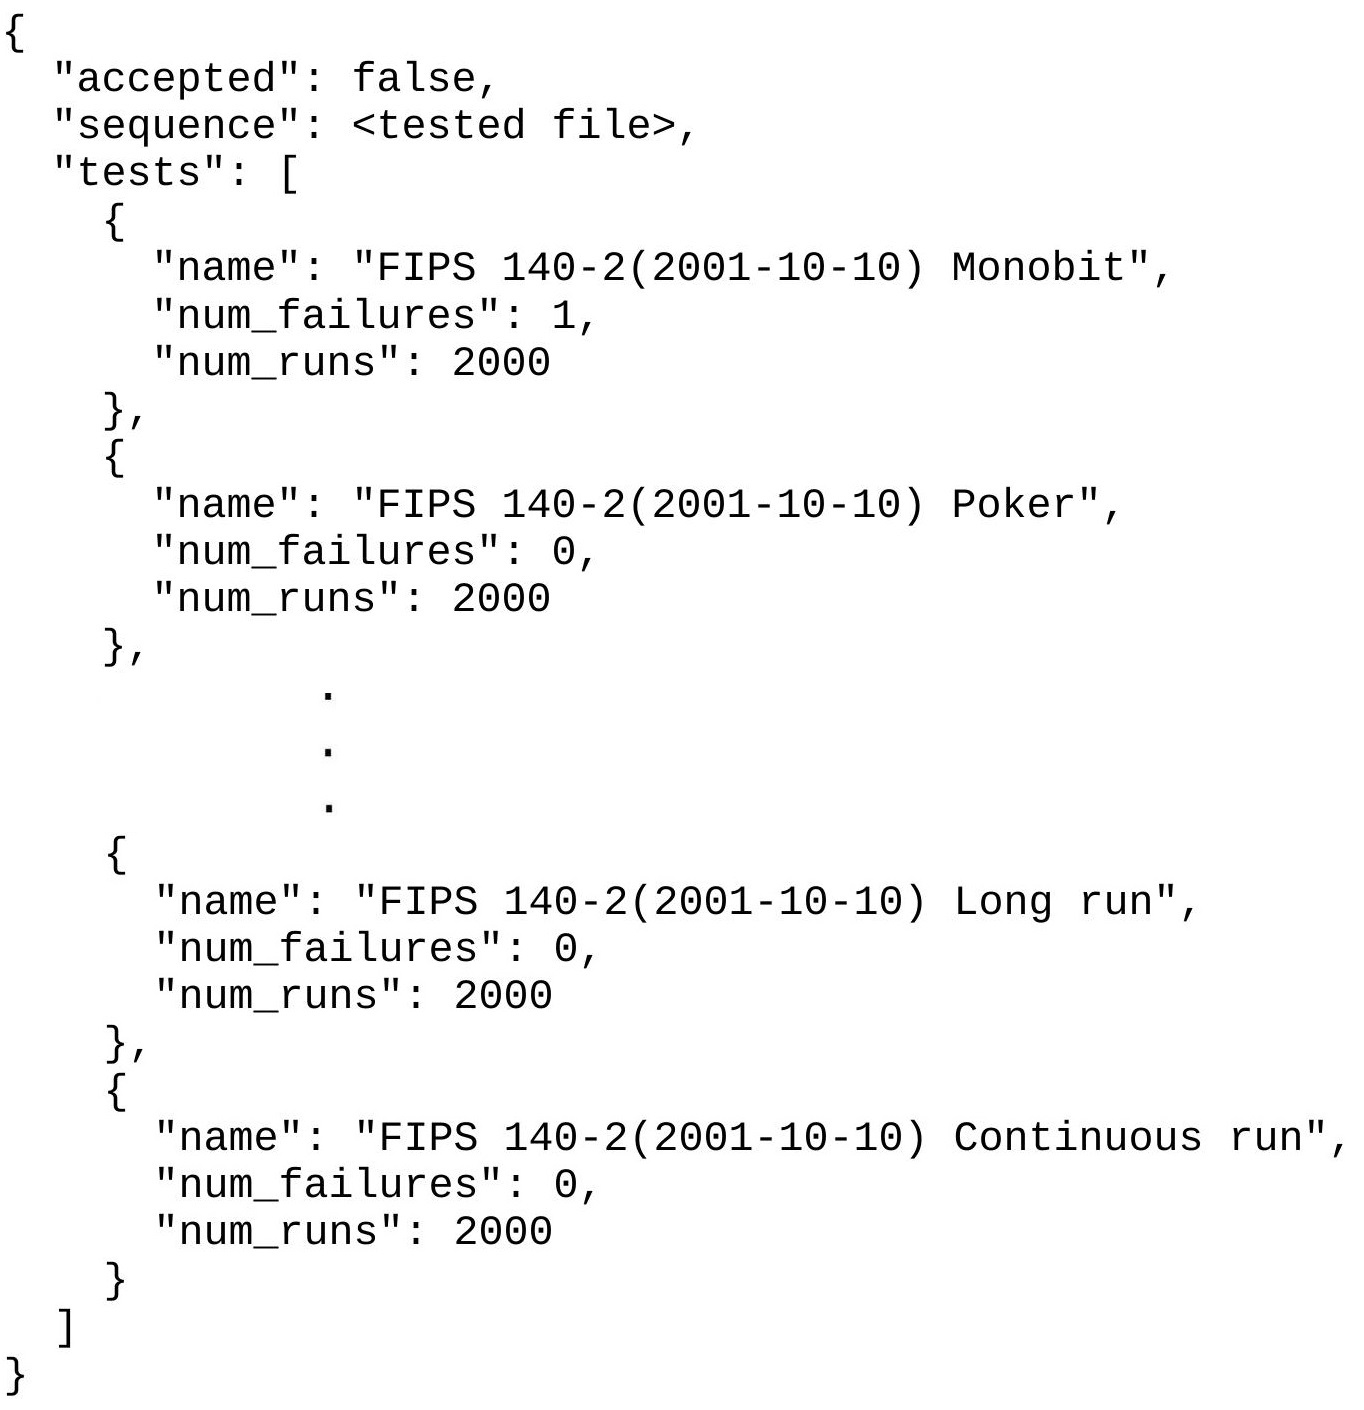
\includegraphics[width=10cm]{figures/outputs-appendix/fips.jpg}
  \end{center}
  \caption{Example of output from \emph{FIPS} battery.}
  \label{fig:fips_example}
\end{figure}

\newpage

\section{BSI battery} \label{append:bsi-output}


\begin{figure}[h!]
  \begin{center}
    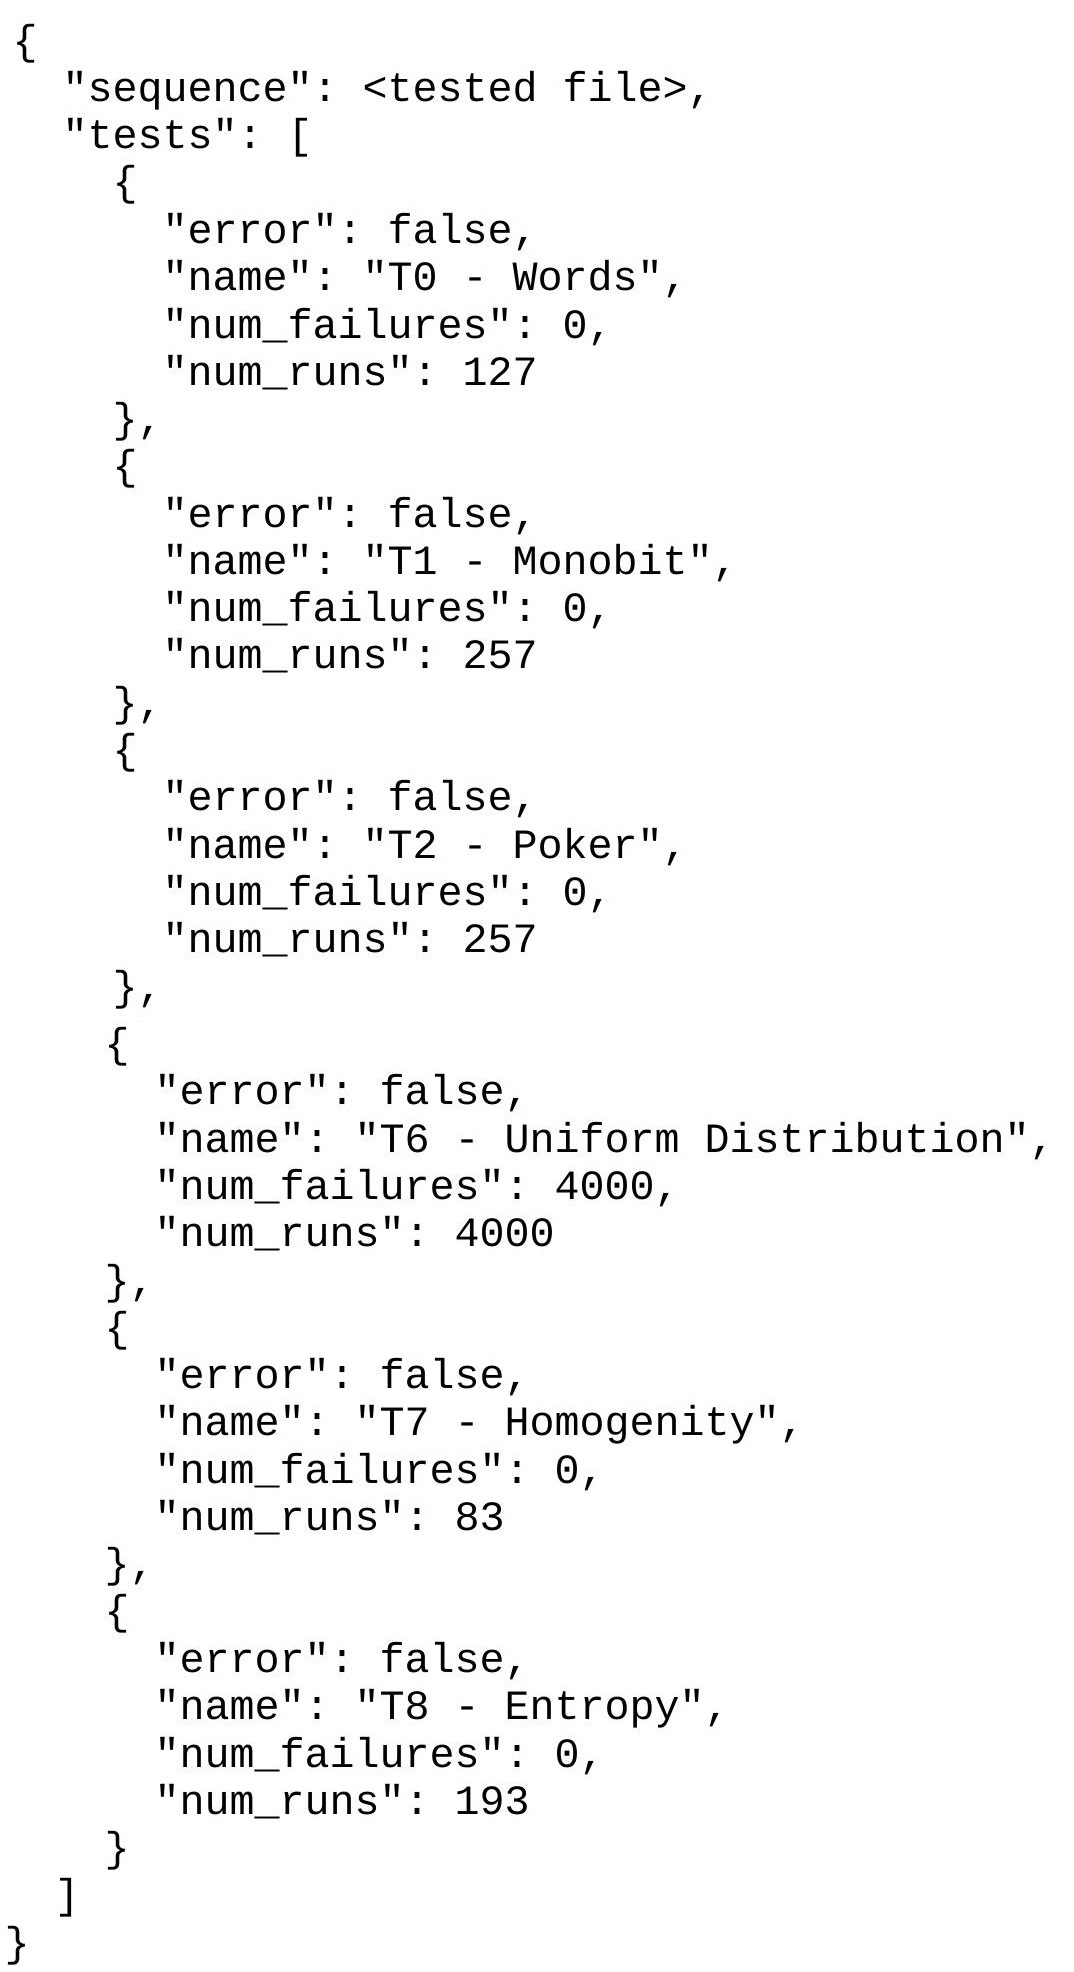
\includegraphics[width=7.5cm]{figures/outputs-appendix/bsi.jpg}
  \end{center}
  \caption{Example of output from \emph{BSI} battery.}
  \label{fig:bsi_example}
\end{figure}

\newpage





\chapter{Examples from testing toolkits} \label{append:rtt}

\section{RTT settings} \label{append:rtt-setting}

\begin{figure}[h!]
  \begin{center}
    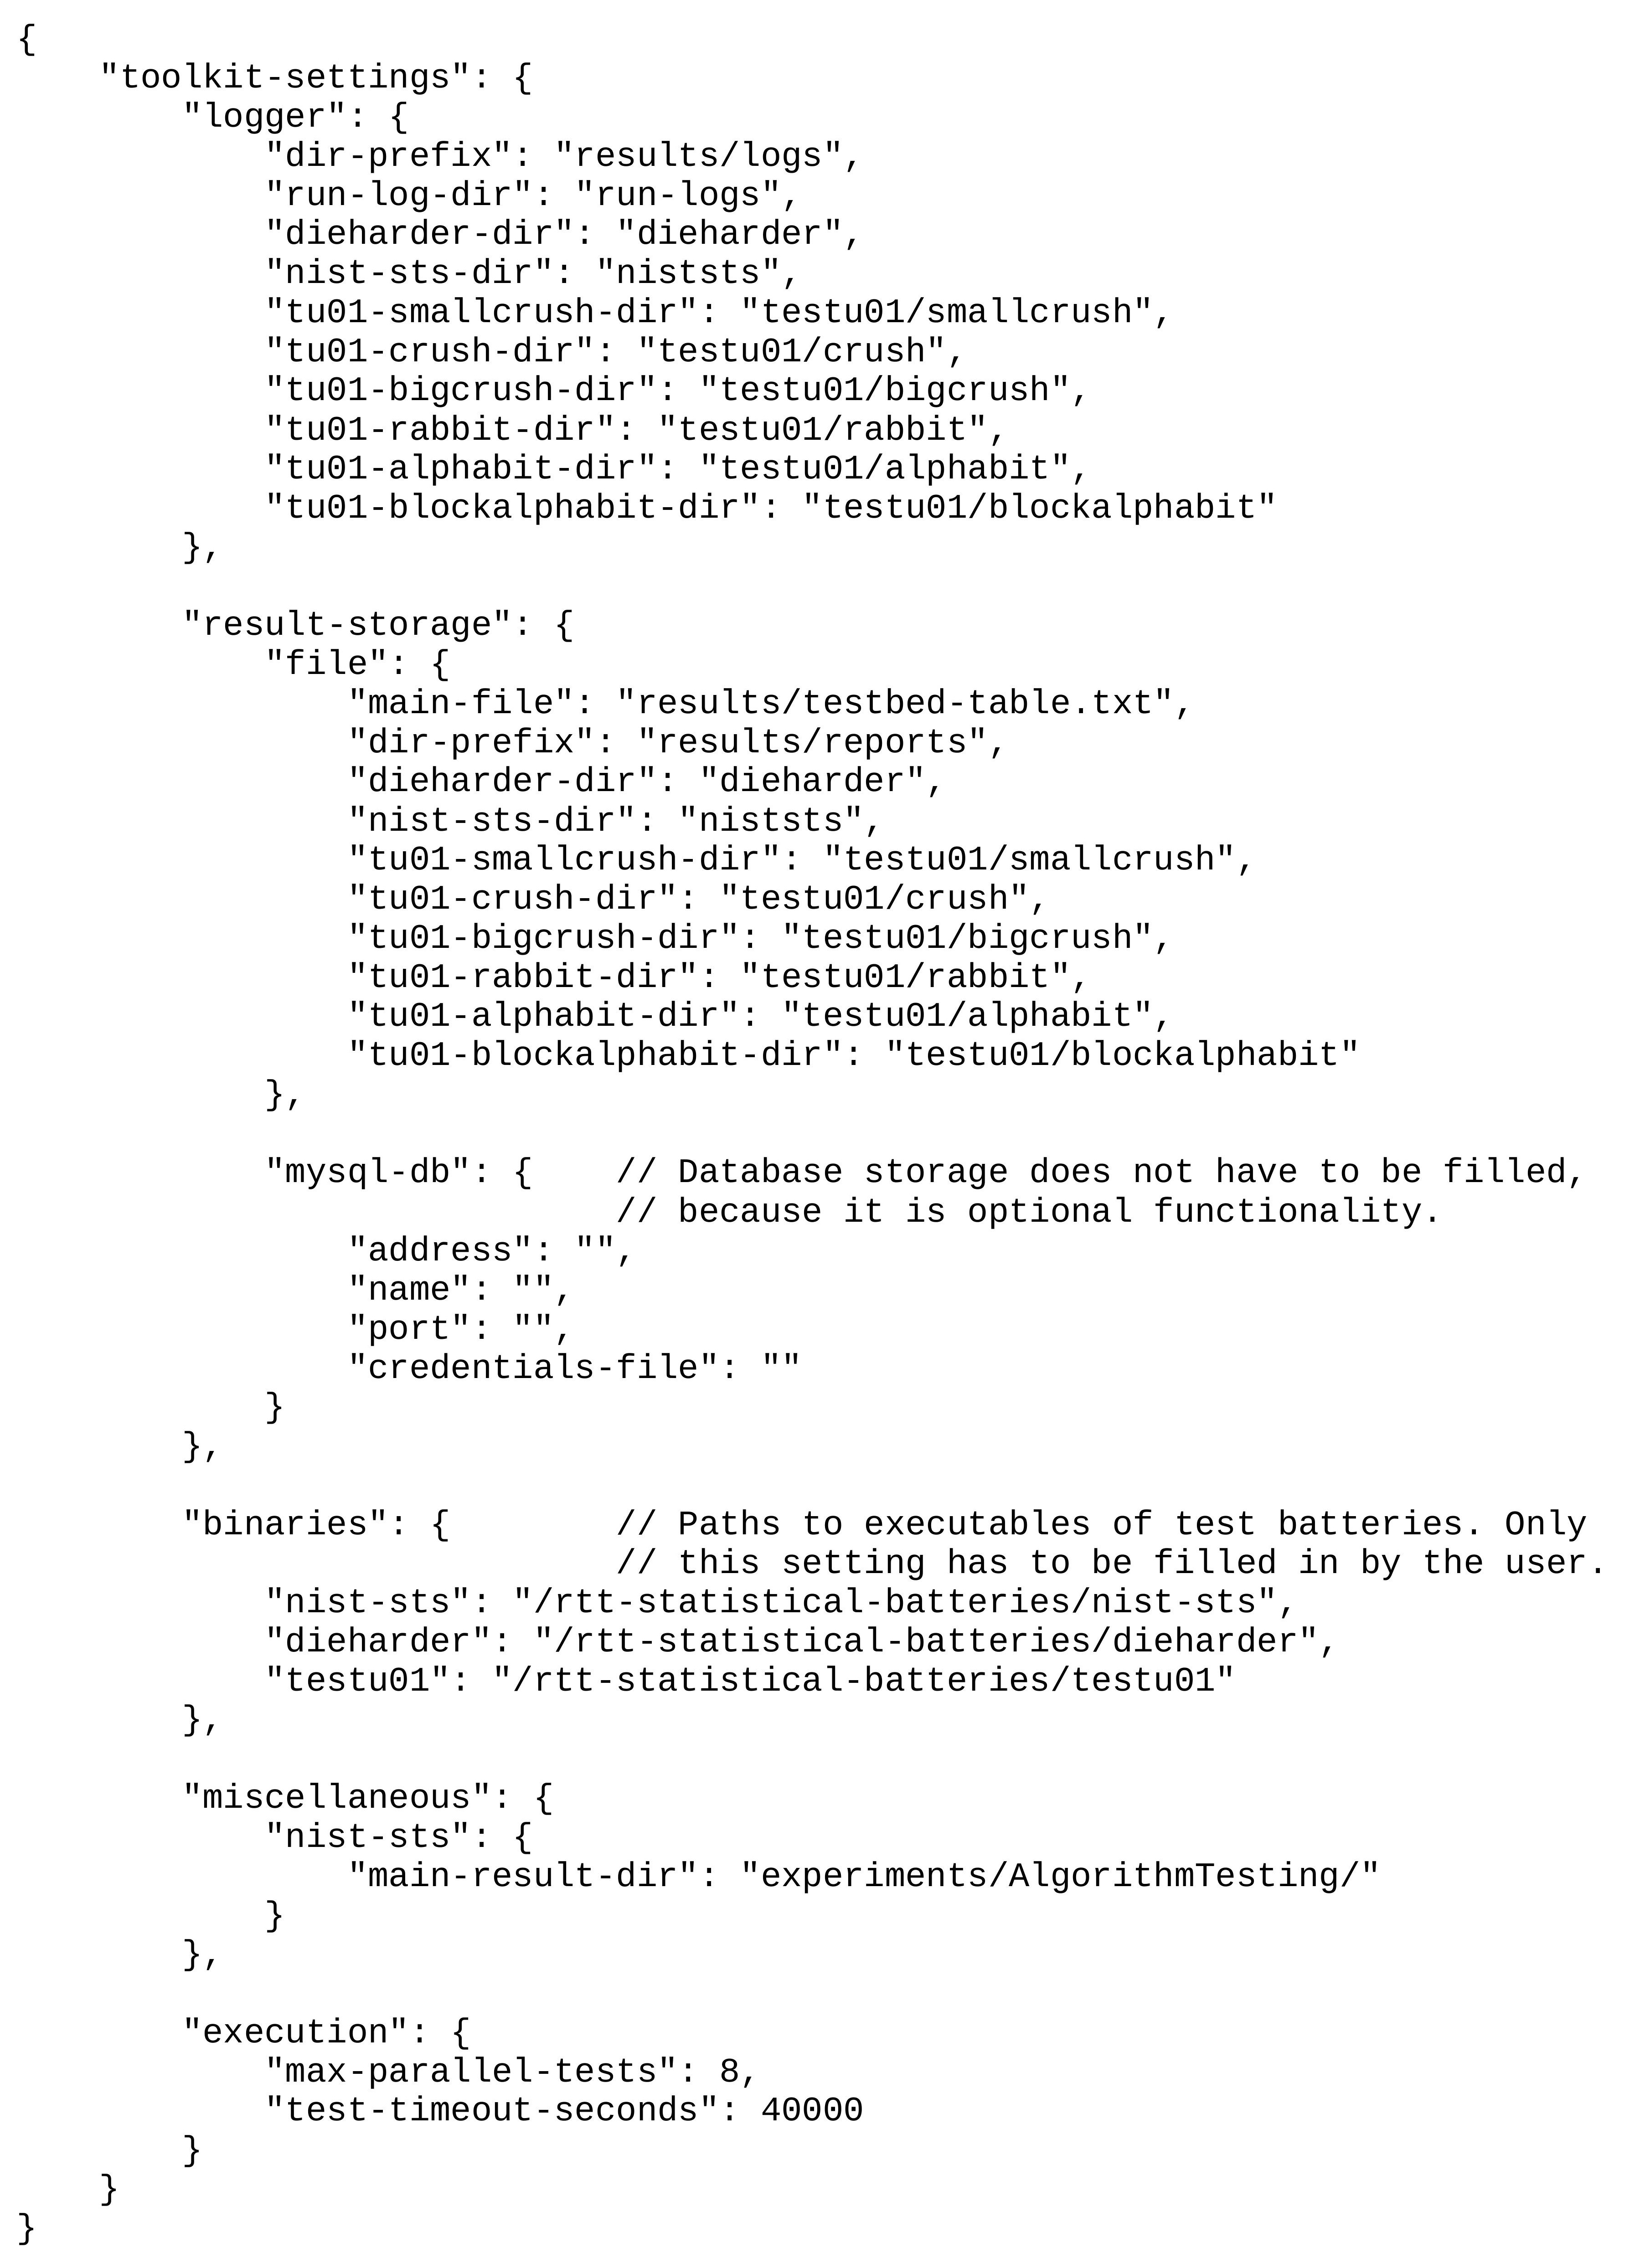
\includegraphics[width=10.9cm]{figures/rtt/rtt-settings.jpg}
  \end{center}
  \caption{General settings for \emph{RTT} stored in \emph{rtt-settings.json} file.}
  \label{fig:rtt_settings}
\end{figure}
\newpage


\section{RTT battery configuration} \label{append:rtt-config}

\begin{figure}[h!]
  \begin{center}
    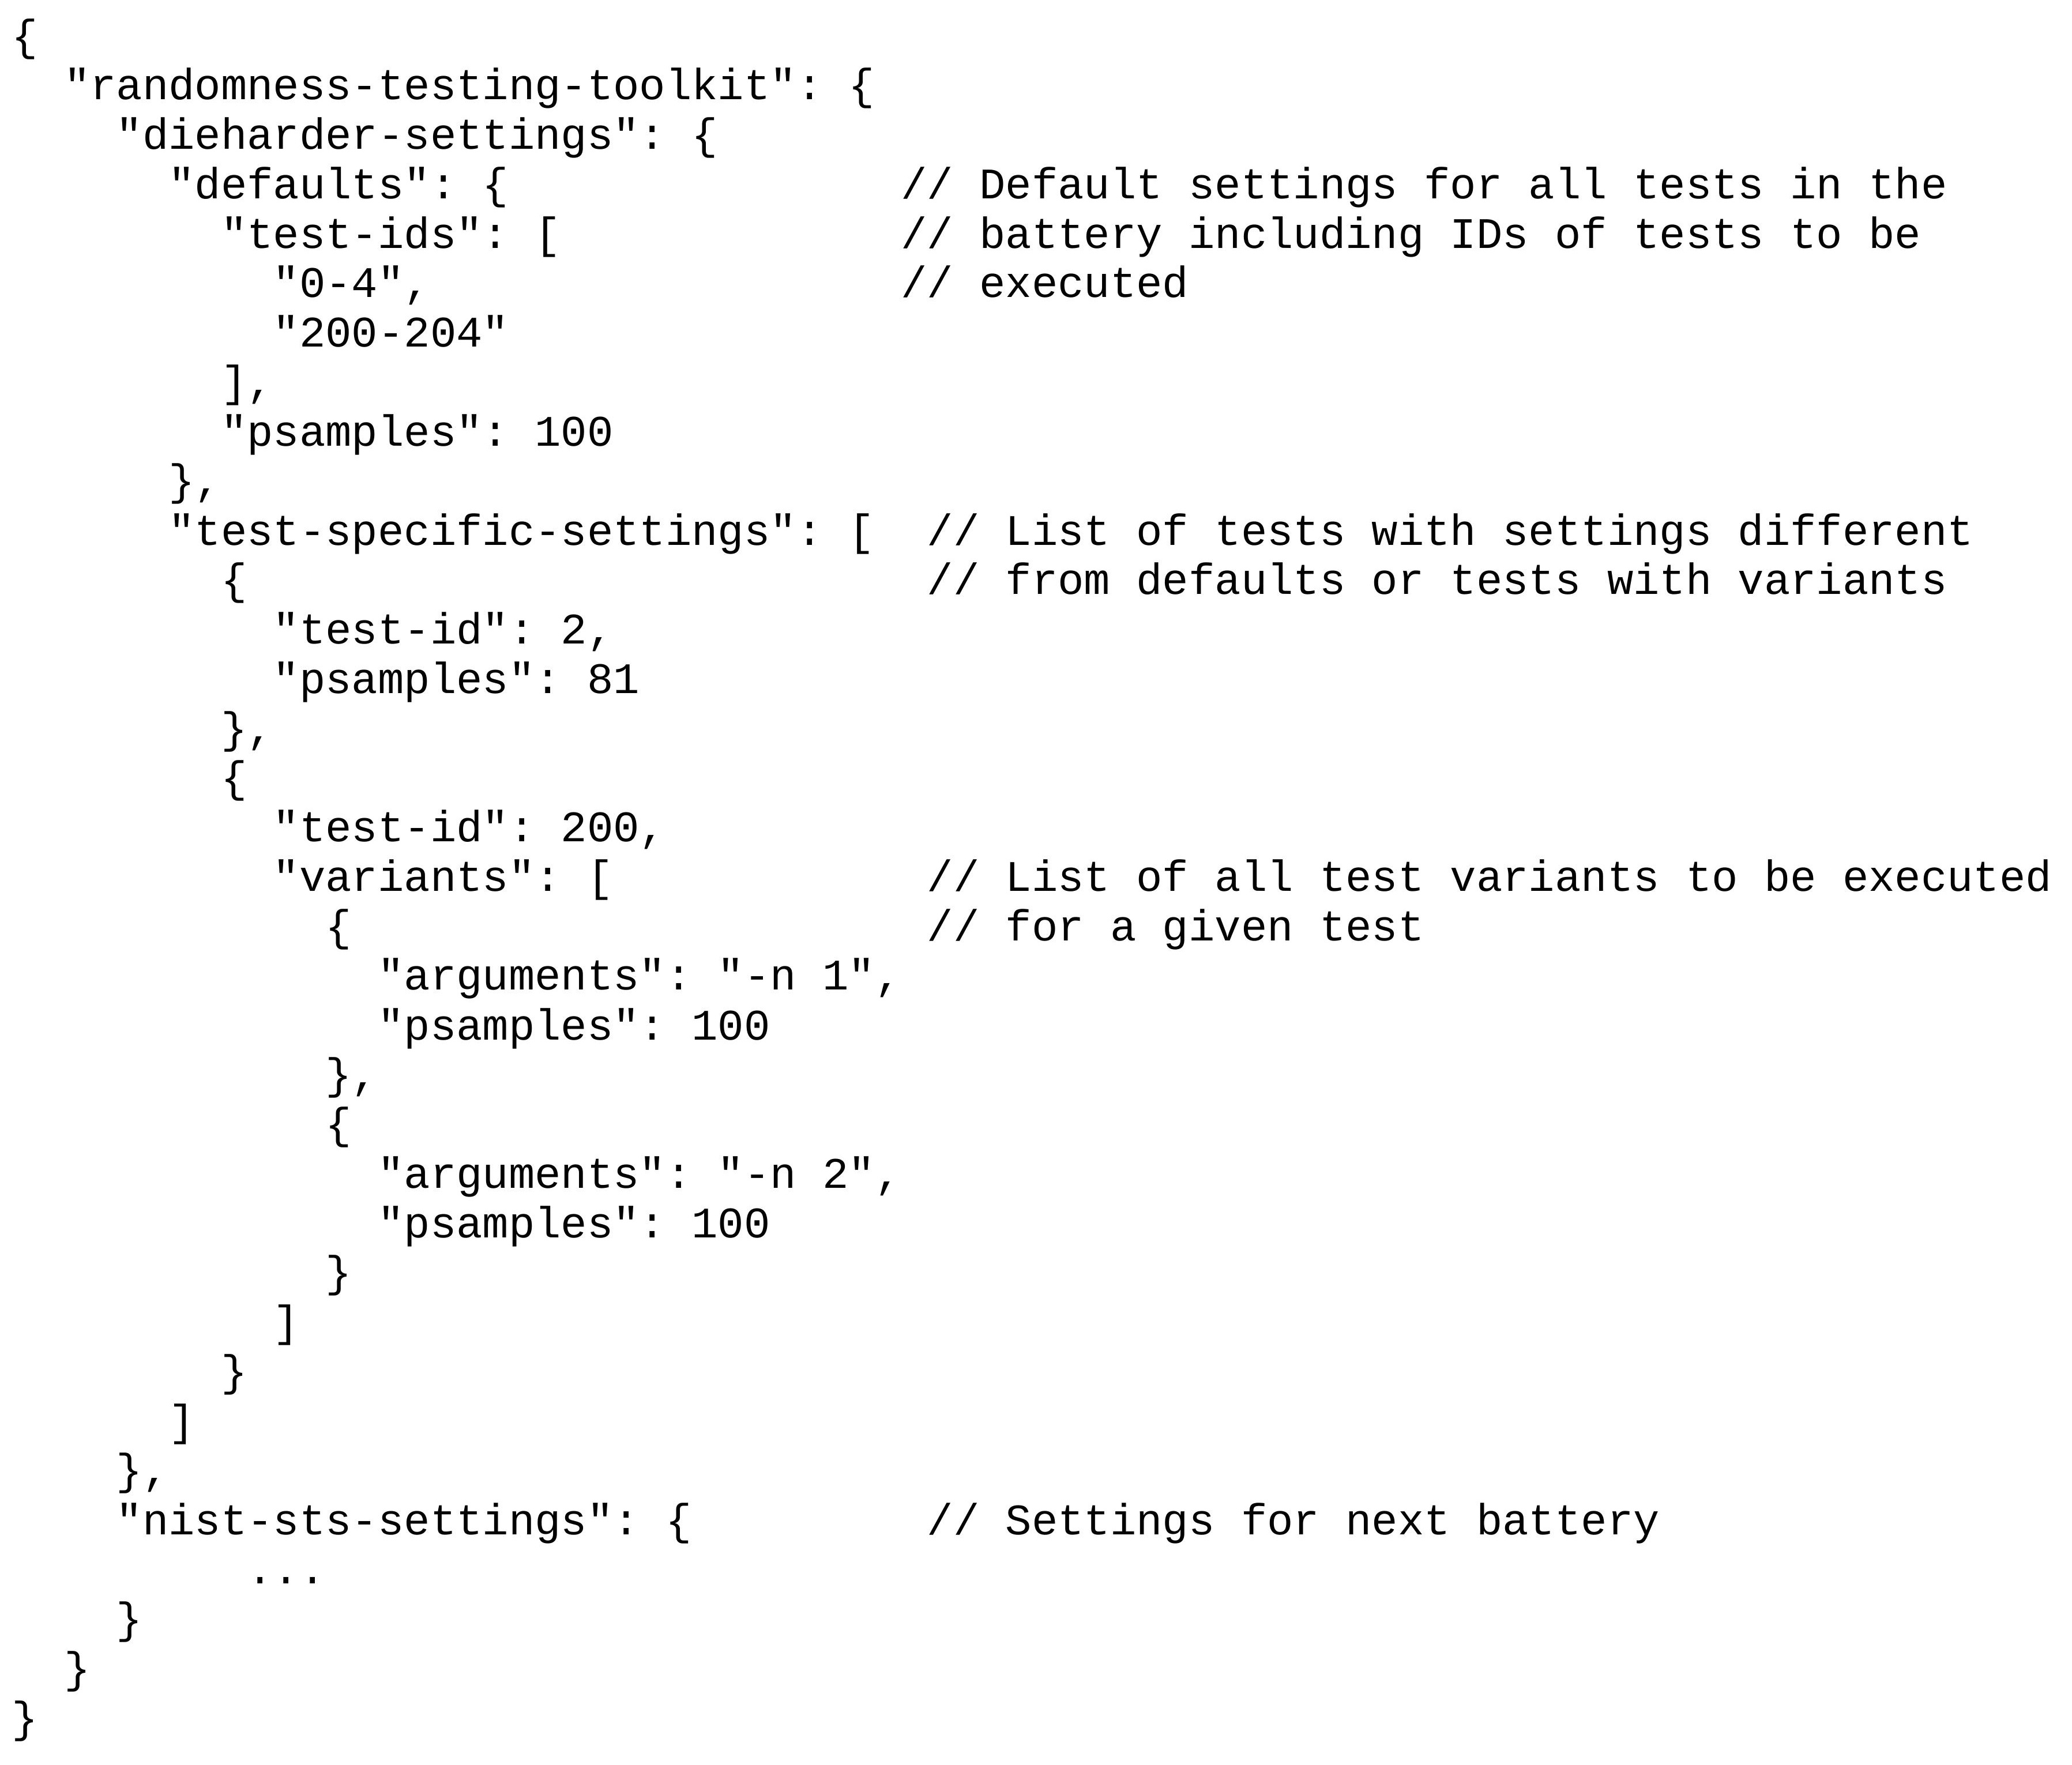
\includegraphics[width=12.5cm]{figures/rtt/config.jpg}
  \end{center}
  \caption{Example of battery configuration file for \emph{RTT}.}
  \label{fig:rtt_config}
\end{figure}

\newpage

\section{Report from \emph{RTT}} \label{append:rtt-output}

\begin{figure}[h!]
  \begin{center}
    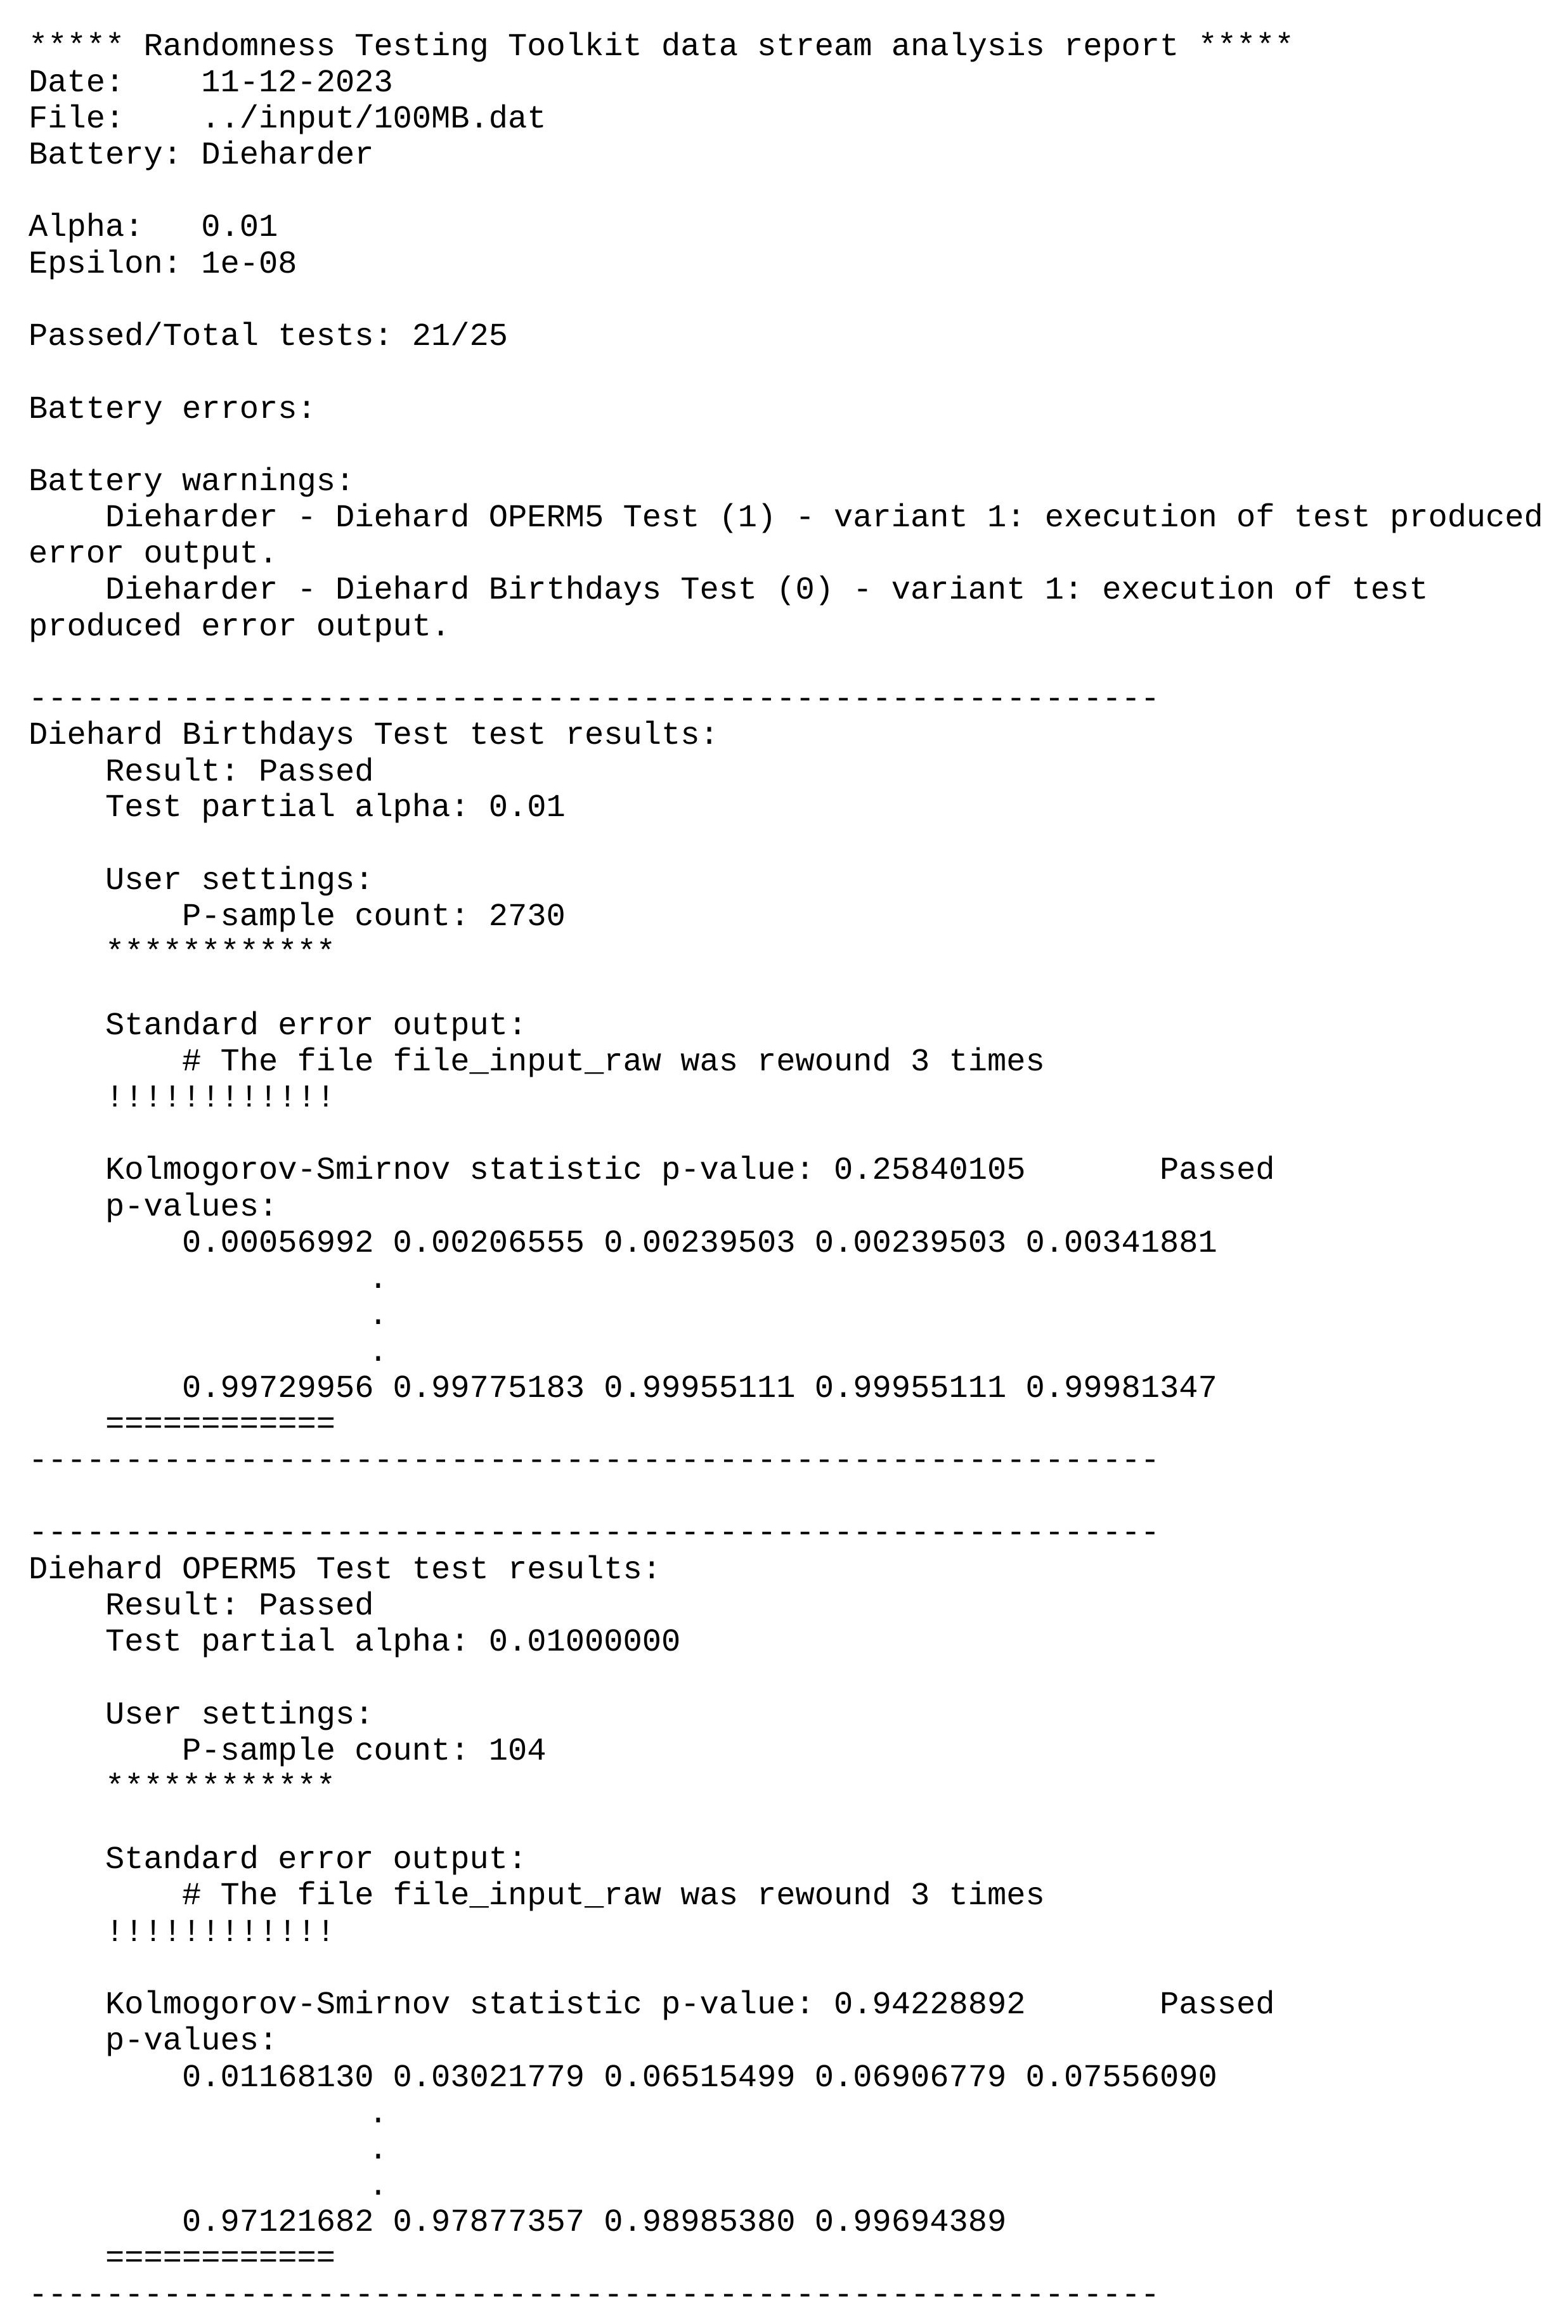
\includegraphics[width=11cm]{figures/rtt/rtt-output.jpg}
  \end{center}
  \caption{Example of report file from \emph{RTT}.}
  \label{fig:rtt_output}
\end{figure}

\newpage

\section{Report from \emph{rtt-py}} \label{append:rtt-py-output}
\begin{figure}[h!]
  \begin{center}
    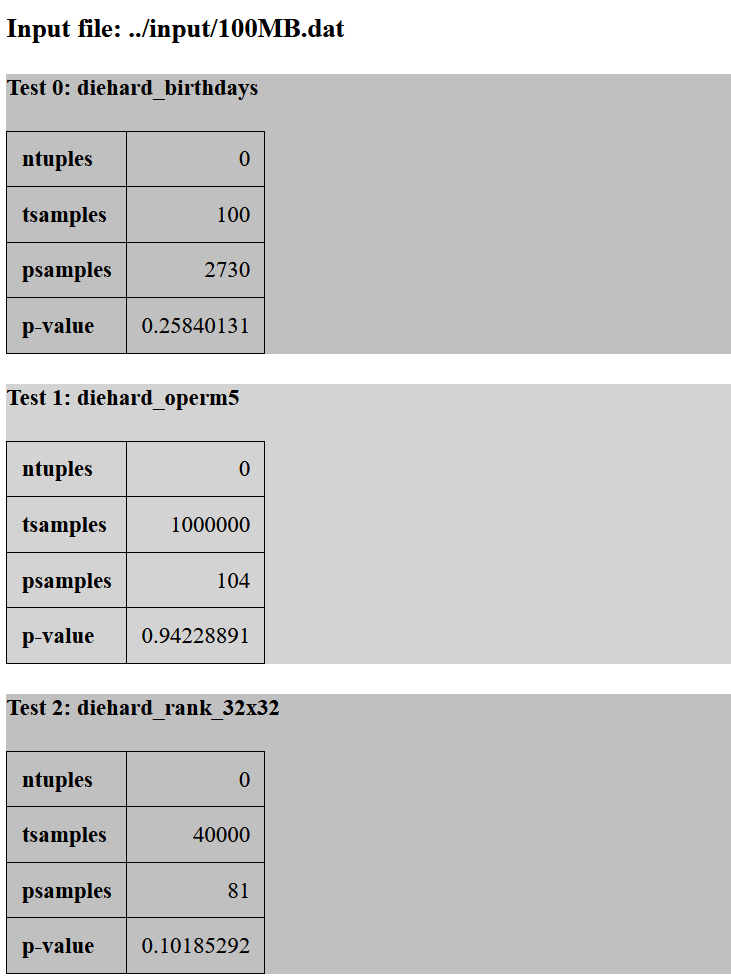
\includegraphics[width=11cm]{figures/rtt/rtt-py-out.png}
  \end{center}
  \caption{Example of HTML report from \emph{rtt-py}.}
  \label{fig:rtt_py_output}
\end{figure}

\newpage

\begin{figure}[h!]
  \begin{center}
    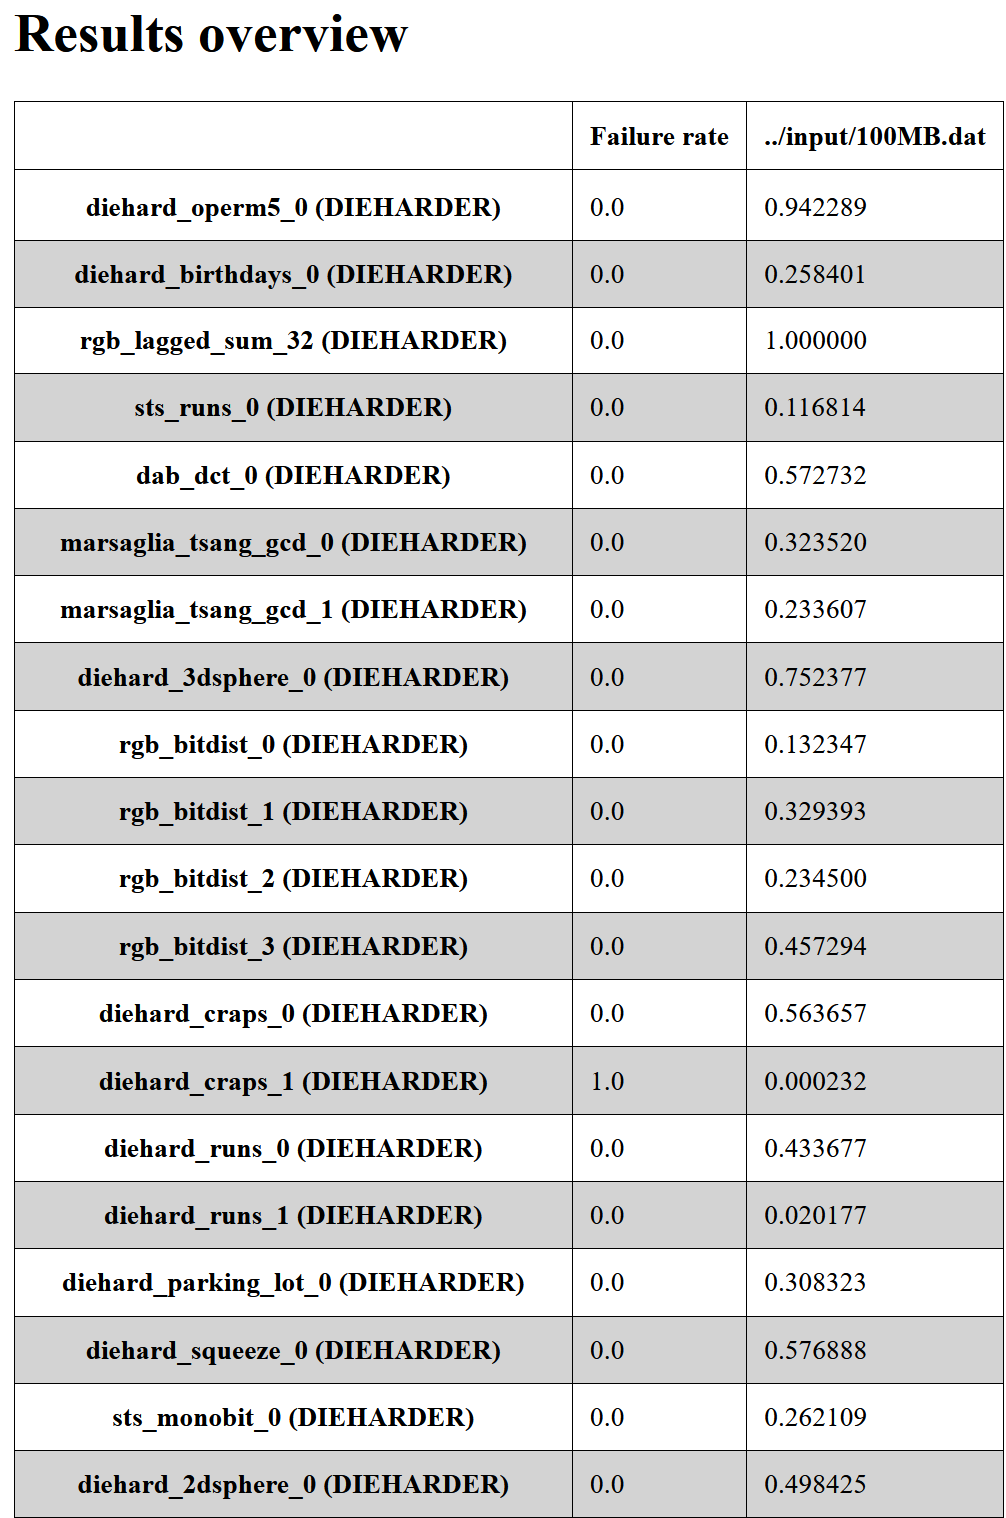
\includegraphics[width=11.5cm]{figures/rtt/rtt-py-table.png}
  \end{center}
  \caption{Example of HTML overview table from \emph{rtt-py}.}
  \label{fig:rtt_py_table_app}
\end{figure}


\end{document}


